% +++
% latex="texfot lualatex-dev"
% +++
\documentclass[body]{subfiles}
\begin{document}
\chapter{実験結果と考察}\label{result}

\section{雲がある場合の全球平均値の太陽定数依存性}

\begin{table}[b]
	\centering
	\caption[雲あり各実験での OLR と OSR の年平均値]{
		雲あり各実験での OLR と OSR の年平均値。
	}\label{OLR-OSR-mean}
	\begin{tblr}{crrr}
		\toprule
		実験&OLR \hmu*{[W/m^{-2}]}&OSR \hmu*{[W/m^{-2}]}&地表面温度 \hmu*{[K]}&平均をとった年度\\
		\midrule
		S1366&\(187.5\)&\(186.8\)&\(286\)&41\\
		S1500&\(190.9\)&\(190.4\)&\(293\)&11\\
		S1600&\(191.1\)&\(193.3\)&\(298\)&11\\
		S1800&\(195.7\)&\(200.3\)&\(307\)&11\\
		S2000&\(184.9\)&\(182.9\)&\(320\)&21\\
		\bottomrule
	\end{tblr}
\end{table}

まず最初に、雲がある場合の実験(実験 S1366, S1500, S1600, S1800, S2000)に
ついて見る。
雲ありの場合について各実験で得られた、全球平均した外向き赤外放射 (OLR) と入射短波放射 (OSR) の
時系列図を図 \ref{time} に示す。この図を見ると、実験 S1366 から S1600
(図 \ref{S1366_OLRA} から \ref{S1600_OLRA})では、おおよそ 10 年以上積分を
することで、全球平均の OLR が季節変化しつつも、全球平均 OLR と OSR が
\(190\hmu{W/m^2}\) 付近でほぼ一致して、大気の状態が平衡になっているよう
にみえる。実験 S1800(図 \ref{S1800_OLRA})でも、OLR と OSR が\(200\hmu{W/m^2}\)
付近の値で一致して、大気の状態が平衡になっているように見える。一方で、S2000
(図 \ref{S2000_OLRA})では、全球平均 OLR が激しく変動している。
表 \ref{OLR-OSR-mean} に OLR と OSR の値の年平均値を示した。
実験 S1366 から S1600 では、OLR と OSR の値の差が \(3.0\hmu{W/m^2}\) 以下
になっていて、この表からも平衡状態に達しているようにみえる。しかし、
実験 S1800 では OLR と OSR の差が \(4.6\hmu{W/m^2}\) と他の実験よりも大きく
なっている。また、S2000 では OLR と OSR の差は \(2.0\hmu{W/m^2}\) と大きくはない。

次に、全球平均地表面温度の時系列図を図 \ref{time} に示す。
全球平均地表面温度は、実験 S1366 から S1600(図 \ref{S1366_SurfTemp} から
\ref{S1600_SurfTemp})では地表面温度がそれぞれ \(286\hmu{K}, 293\hmu{K}, 298\hmu{K}\)
で一定となり、平衡状態に達しているように見える。しかし、実験 S1800 では
地表面温度が上昇し続けていて、平衡状態に達していないようにみえる。
また、実験 S2000 では、地表面温度が \(320\hmu{K}\) で一定になっている
ように見える。

以上のことから、実験 S1366, S1500, S1600 は平衡状態に達しているが、
実験 S1800 は全球平均 OLR と OSR に差があり、地表面温度が上昇し続けていて
平衡状態に達していない。また、実験 S2000 に関しては、全球平均値を見ただけでは
判断できないが、これから示すように平衡状態になっておらず、大気の状態を
正しく表現できていない可能性がある。

次に、雲あり各実験での OLR の東西平均を図 \ref{OLRA東西平均} に、地表面温度の
東西平均を図 \ref{地表面温度} に示す。
図 \ref{OLRA東西平均} を見ると、実験 S1366 から S1800 までは、OLR の
東西平均の南北分布に特徴的なパターンがあるのが見える。低緯度では OLR の値が
小さく、中緯度で大きくなり、高緯度で小さくなっている。赤道での OLR の値は、
実験 S1366, S1500, S1600, S1800 の順で、
\(125\hmu{W/m^2},135\hmu{W/m^2},145\hmu{W/m^2},175\hmu{W/m^2}\)
となっていて、中緯度のピークの値はそれぞれ南半球・北半球ともに
\(240\hmu{W/m^2},250\hmu{W/m^2},245\hmu{W/m^2},238\hmu{W/m^2}\)
となって、そのピークが現れる緯度が高緯度側に移動している。実験 S2000 では他の
実験とは違い、低緯度で OLR の値が小さくなっておらず、中緯度にもピークが
現れておらず、他の実験とは異なるパターンになっている。このように、OLR の
値は実験 S1366 から S1600 までは太陽定数が大きくなるにつれて南北の差が小さく
なっている。
地表面温度(図 \ref{地表面温度})を見ると、どの実験でも赤道で地表面温度が
高く、極で地表面温度が低くなっている。赤道での地表面温度は、
実験 S1366, S1500, S1600, S1800, S2000 の順で、
\(296\hmu{K},302\hmu{K},306\hmu{K},314\hmu{K},324\hmu{K}\)
となっている。極での地表面温度はそれぞれ
\(270\hmu{K},281\hmu{K},288\hmu{K},298\hmu{K},317\hmu{K}\)
となっている。極と赤道の地表面温度の差はぞれぞれ、
\(14\hmu{K},19\hmu{K},18\hmu{K},16\hmu{K},7\hmu{K}\)
となっていて、実験 S1366 から S1500 にかけては地表面温度の南北差が一旦大きく
なっているが、実験 S1600 では小さくなっている。

以上のことから、実験 S1366, S1500, S1600 に関しては、
灰色大気・雲なしのモデルで Ishiwatari \etal (2002) が結論したように、
非灰色大気・雲ありのモデルでも、太陽定数の増大に伴って、南北に一様になる
ということが言えよう。

実験 S1800 では、先述したように、OLR と OSR の差が大きく、地表面温度が時間
に応じて増大している。したがって、実験 S1800 では暴走温室状態になっている
と考えられる。実験 S2000 で OLR の東西平均が他の太陽定数とは異なっている
パターンを示しているのは、この実験でも暴走温室状態になっており、大気の状態
が正しく表現されていないものと想像できる。
そのため、実験 S1800, S2000 に関しては、
積分時間をさらに延長しなければ詳しく議論をすることはできないだろう。

\begin{figure}[t]
	\centering
	\begin{subfigure}{.4\textwidth}
		\centering
		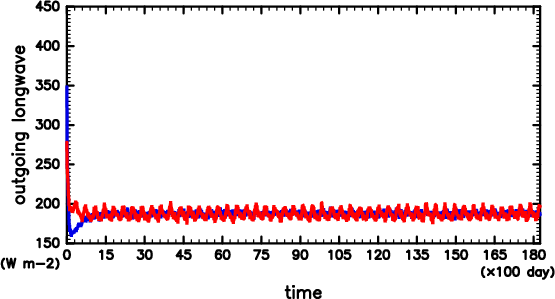
\includegraphics[width=\textwidth]{S1366/S1366_OLRA-OSRA_horimean_time0.0-18250.0-crop.png}
		\caption{S1366 (OLR, OSR)}\label{S1366_OLRA}
	\end{subfigure}
	\begin{subfigure}{.4\textwidth}
		\centering
		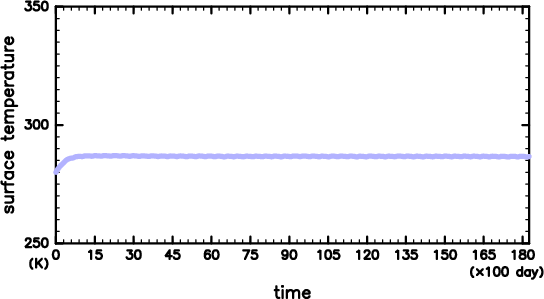
\includegraphics[width=\textwidth]{S1366/S1366_SurfTemp_horimean_time0.0-18250.0-crop.png}
		\caption{S1366(地表面温度)}\label{S1366_SurfTemp}
	\end{subfigure}
	\begin{subfigure}{.4\textwidth}
		\centering
		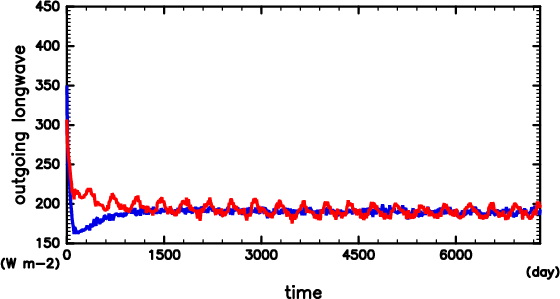
\includegraphics[width=\textwidth]{S1500/S1500_OLRA-OSRA_horimean_time0.0-7300.0-crop.png}
		\caption{S1500 (OLR, OSR)}\label{S1500_OLRA}
	\end{subfigure}
	\begin{subfigure}{.4\textwidth}
		\centering
		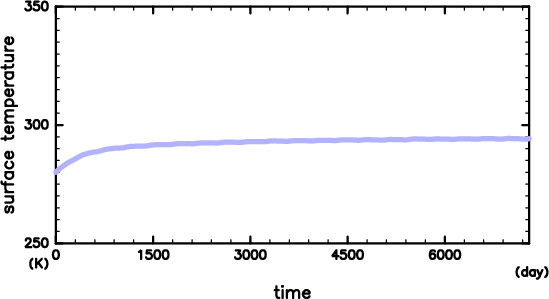
\includegraphics[width=\textwidth]{S1500/S1500_SurfTemp_horimean_time0.0-7300.0-crop.png}
		\caption{S1500(地表面温度)}\label{S1500_SurfTemp}
	\end{subfigure}
	\begin{subfigure}{.4\textwidth}
		\centering
		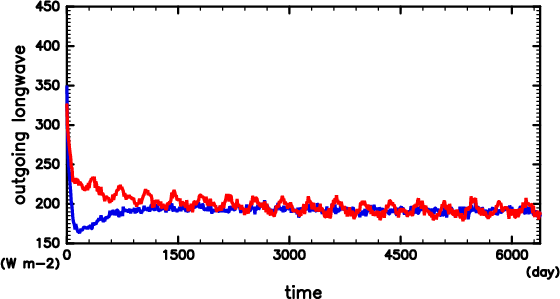
\includegraphics[width=\textwidth]{S1600/S1600_OLRA-OSRA_horimean_time0.0-7300.0-crop.png}
		\caption{S1600 (OLR, OSR)}\label{S1600_OLRA}
	\end{subfigure}
	\begin{subfigure}{.4\textwidth}
		\centering
		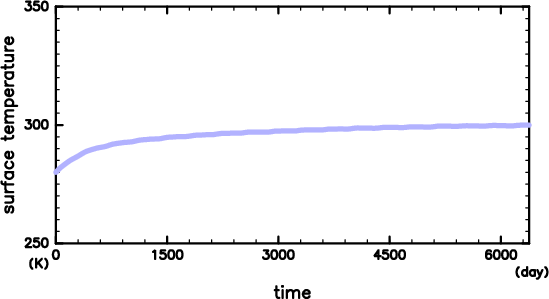
\includegraphics[width=\textwidth]{S1600/S1600_SurfTemp_horimean_time0.0-7300.0-crop.png}
		\caption{S1600(地表面温度)}\label{S1600_SurfTemp}
	\end{subfigure}
	\begin{subfigure}{.4\textwidth}
		\centering
		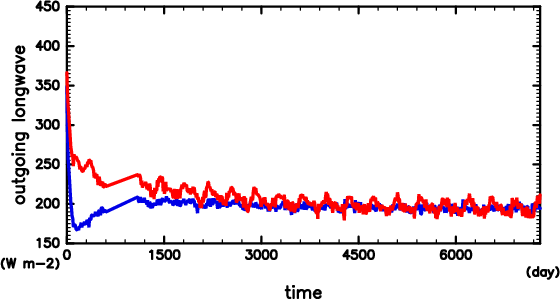
\includegraphics[width=\textwidth]{S1800/S1800_OLRA-OSRA_horimean_time0.0-7300.0-crop.png}
		\caption{S1800 (OLR, OSR)}\label{S1800_OLRA}
	\end{subfigure}
	\begin{subfigure}{.4\textwidth}
		\centering
		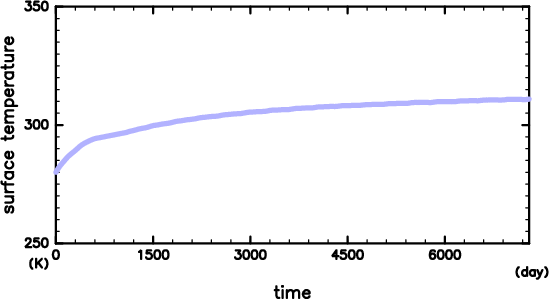
\includegraphics[width=\textwidth]{S1800/S1800_SurfTemp_horimean_time0.0-7300.0-crop.png}
		\caption{S1800(地表面温度)}\label{S1800_SurfTemp}
	\end{subfigure}
	\begin{subfigure}{.4\textwidth}
		\centering
		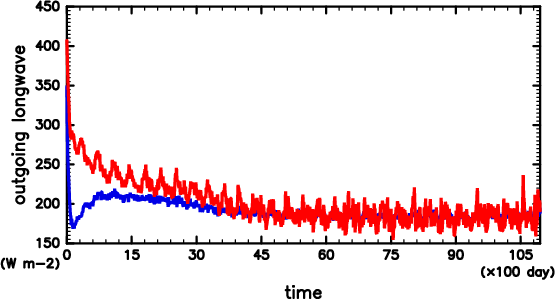
\includegraphics[width=\textwidth]{S2000/S2000_OLRA-OSRA_horimean_time0.0-10950.0-crop.png}
		\caption{S2000 (OLR, OSR)}\label{S2000_OLRA}
	\end{subfigure}
	\begin{subfigure}{.4\textwidth}
		\centering
		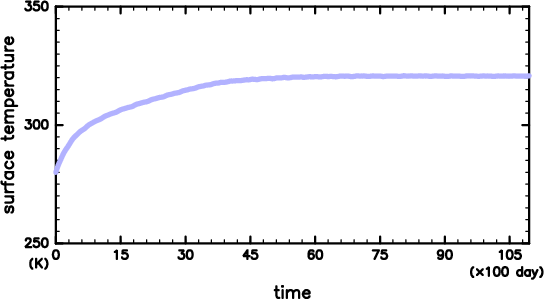
\includegraphics[width=\textwidth]{S2000/S2000_SurfTemp_horimean_time0.0-10950.0-crop.png}
		\caption{S2000(地表面温度)}\label{S2000_SurfTemp}
	\end{subfigure}
	\caption[雲あり各実験での全球平均 OLR, OSR, 地表面温度の時系列変化]{
		(\subref{S1366_OLRA}, \subref{S1500_OLRA}, \subref{S1600_OLRA},
		\subref{S1800_OLRA}, \subref{S2000_OLRA})
		雲あり各実験での全球平均した OLR(赤線)と OSR(青線)の時系列変化。
		横軸は時刻で、縦軸は OLR, OSR の値 \hmu*{[W/m^{2}]}。
		(\subref{S1366_SurfTemp}, \subref{S1500_SurfTemp}, \subref{S1600_SurfTemp},
		\subref{S1800_SurfTemp}, \subref{S2000_SurfTemp})
		雲あり各実験での全球平均地表面温度の時系列変化。
		横軸は時刻で、縦軸は全球平均地表面温度 \hmu*{[K]}。
	}\label{time}
\end{figure}

\begin{figure}[t]
	\centering
	\begin{subfigure}{.45\textwidth}
		\centering
		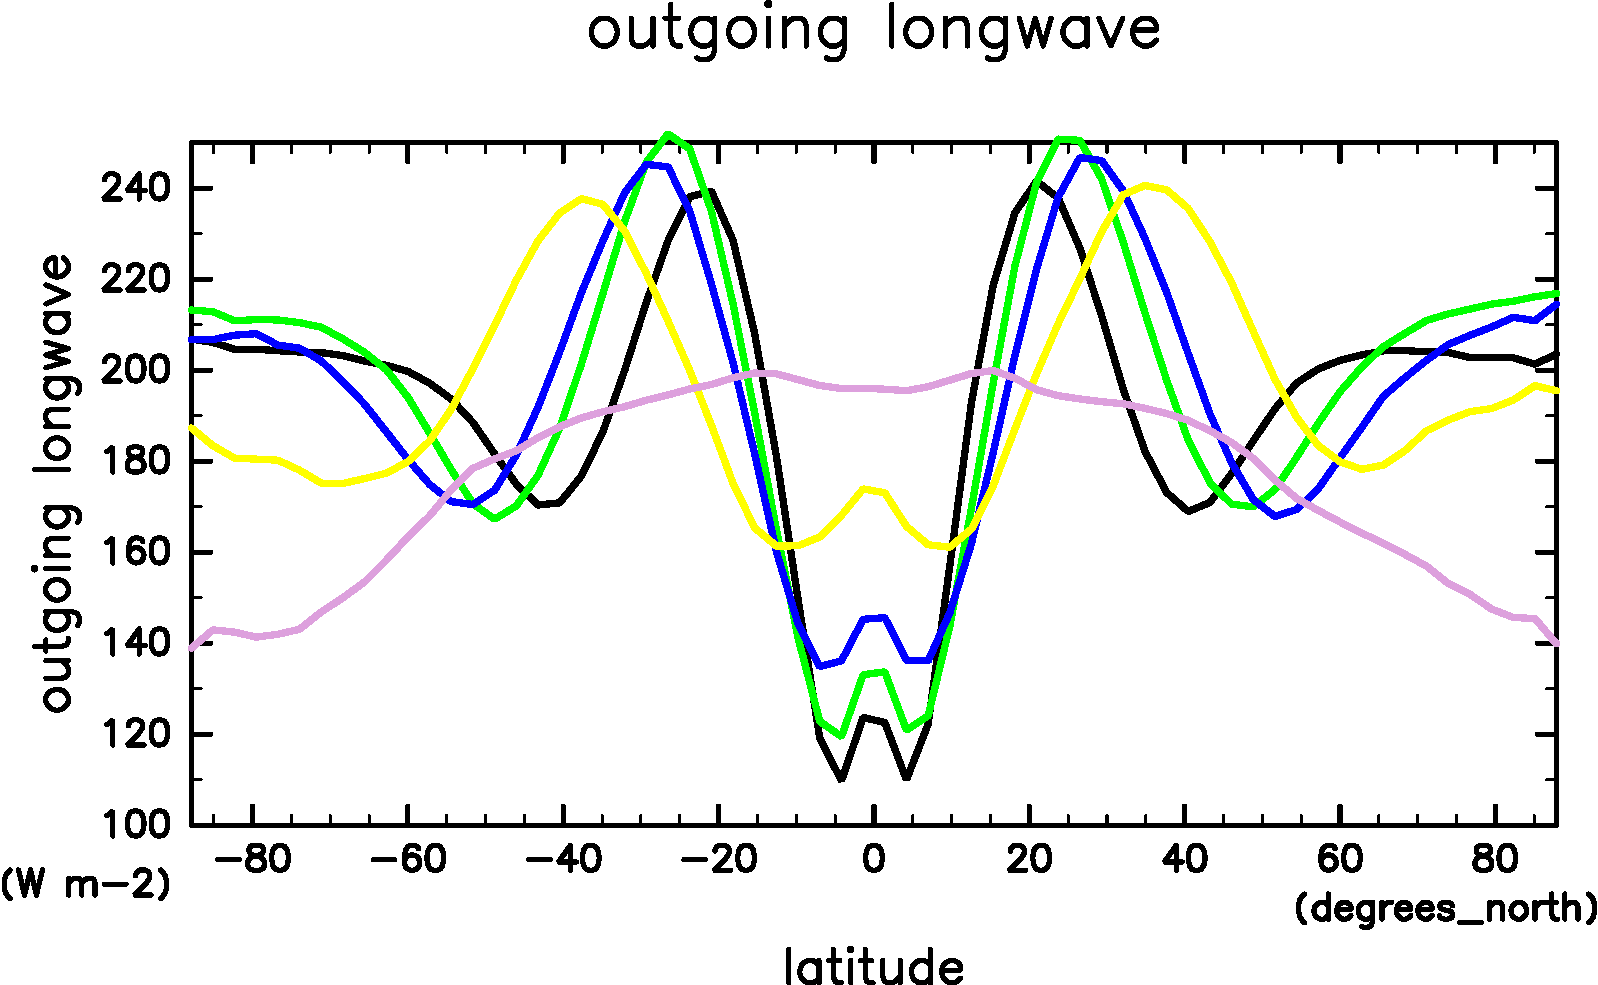
\includegraphics[width=\textwidth]{OLR-overplot-crop-rotate.pdf}
		\caption{OLR の東西平均}\label{OLRA東西平均}
	\end{subfigure}
	\hfill
	\begin{subfigure}{.45\textwidth}
		\centering
		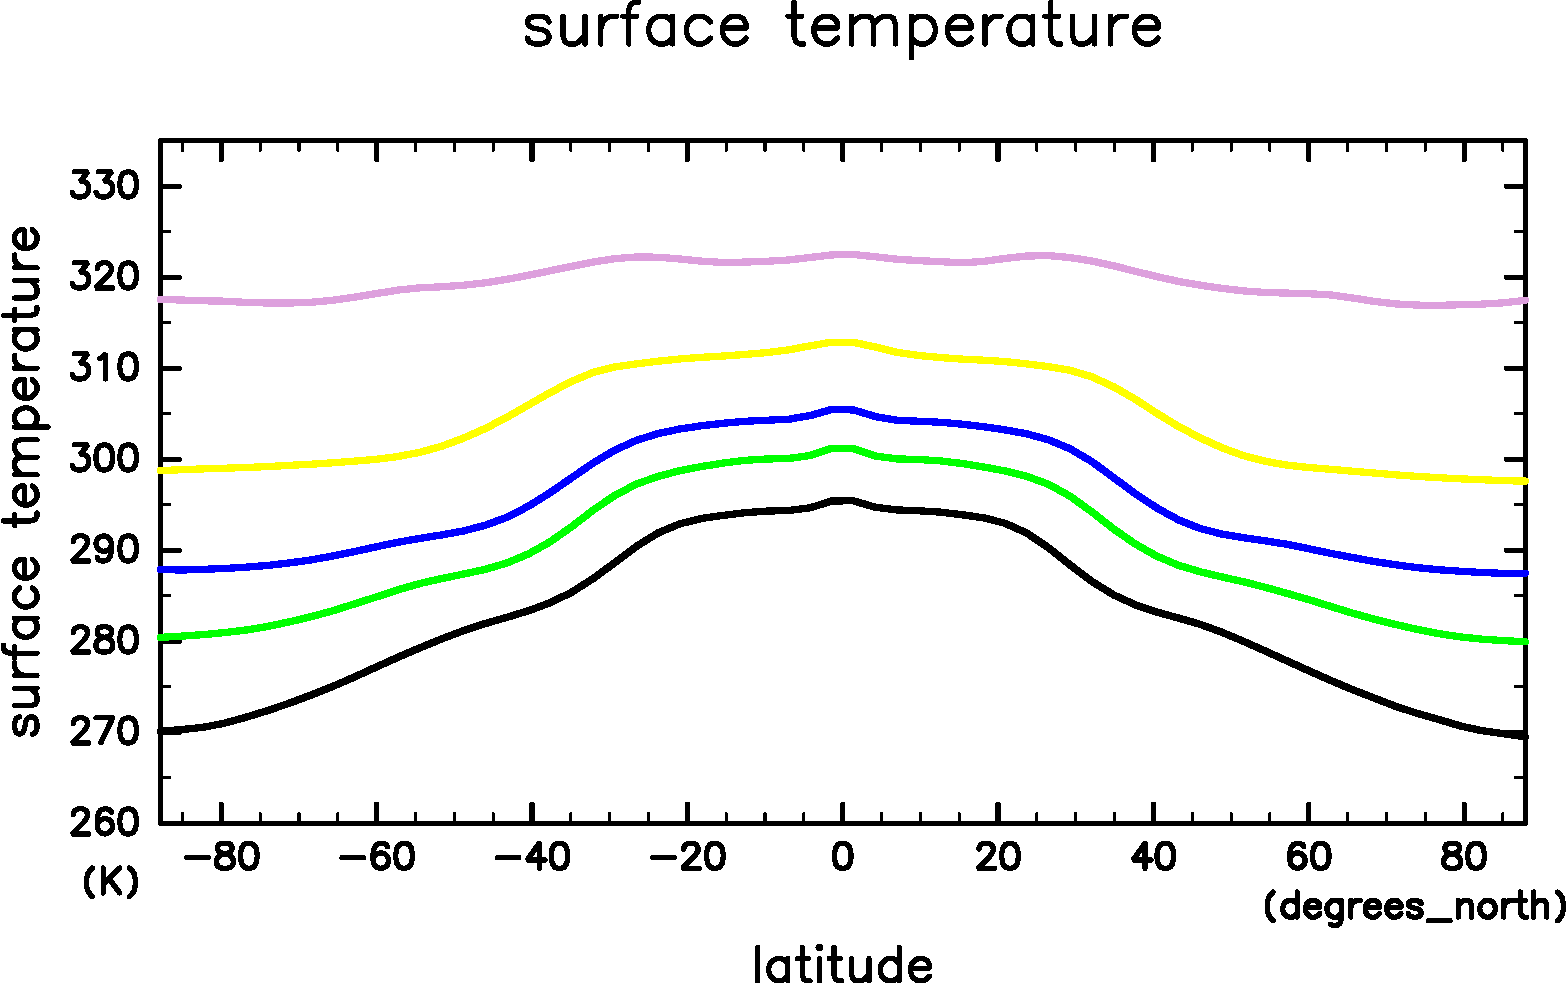
\includegraphics[width=\textwidth]{SurfTemp-overplot-crop-rotate.pdf}
		\caption{地表面温度の東西平均}\label{地表面温度}
	\end{subfigure}
	\caption[雲あり各実験での OLR と地表面温度の東西平均]{
		雲あり各実験での OLR と地表面温度の東西平均の南北分布。
		それぞれ年平均した値で、
		黒線: S1366; 緑線: S1500; 青線: S1600; 黄線: S1800; 桃線: S2000 の結果である。
		横軸は緯度で、縦軸はそれぞれ (\subref{OLRA東西平均}) OLR の東西平均 \hmu*{[W/m^2]}と、
		(\subref{地表面温度}) 地表面温度の東西平均 \hmu*{[K]} である。
	}
\end{figure}

\afterpage{\clearpage}

\section{雲がある場合の大気構造の太陽定数依存性}

次に、雲あり各実験で得られた大気構造がどのようになっているか詳細に見てゆこう。
雲あり各実験で得られた子午面構造を図 \ref{S1366} から \ref{S2000} に示す。
東西風の子午面分布(図 \ref{S1366東西風} から \ref{S2000東西風})を見ると、
いずれも南北で対称な分布となっていて、
実験 S1366(図 \ref{S1366東西風})では緯度 30\textdegree 、\(\sigma=0.1\) に \(60\hmu{m/s}\) の、
実験 S1500(図 \ref{S1500東西風})では緯度 40\textdegree 、\(\sigma=0.1\) に \(70\hmu{m/s}\) の、
実験 S1600(図 \ref{S1600東西風})では緯度 40\textdegree 、\(\sigma=0.05\) に \(80\hmu{m/s}\) の、
実験 S1800(図 \ref{S1800東西風})では緯度 50\textdegree 、\(\sigma=0.0\) に \(90\hmu{m/s}\) の、
実験 S2000(図 \ref{S2000東西風})では緯度 40\textdegree 、\(\sigma=0.0\) に \(80\hmu{m/s}\) の
東向きの風が吹いている。このことから、実験 S1366 から S1600 ではジェットが
発生していることがわかる。しかし、S1800 と S2000 ではジェットが大気上端に
達しており、モデルの高度が足りていない可能性がある。

子午面の循環構造に関しても見てゆこう。図 \ref{S1366南北風} から \ref{S2000南北風}
に南北風の子午面分布を、図 \ref{S1366質量流線関数} から \ref{S2000質量流線関数} に
質量流線関数の子午面分布を示す。地表面付近の南北風は、いずれも南北で対称な分布となっていて、
実験 S1366(図 \ref{S1366南北風})では緯度 10\textdegree で \(5\hmu{m/s}\) の、
実験 S1500(図 \ref{S1500南北風})では緯度 10\textdegree で \(5\hmu{m/s}\) の、
実験 S1600(図 \ref{S1600南北風})では緯度 13\textdegree で \(4\hmu{m/s}\) の、
実験 S1800(図 \ref{S1800南北風})では緯度 20\textdegree で \(2\hmu{m/s}\) の、
実験 S2000(図 \ref{S2000南北風})では緯度 10\textdegree で \(0.5\hmu{m/s}\) の
低緯度向きの風が吹いている。また、
実験 S1366(図 \ref{S1366南北風})では緯度 35\textdegree で \(3\hmu{m/s}\) の、
実験 S1500(図 \ref{S1500南北風})では緯度 40\textdegree で \(3.5\hmu{m/s}\) の、
実験 S1600(図 \ref{S1600南北風})では緯度 43\textdegree で \(4\hmu{m/s}\) の、
実験 S1800(図 \ref{S1800南北風})では緯度 50\textdegree で \(2\hmu{m/s}\) の、
実験 S2000(図 \ref{S2000南北風})では緯度 40\textdegree で \(0.5\hmu{m/s}\) の
高緯度向きの風が吹いている。高高度では、
実験 S1366(図 \ref{S1366東西風})では緯度 10\textdegree 、\(\sigma=0.2\) に \(3\hmu{m/s}\) の、
実験 S1500(図 \ref{S1500東西風})では緯度 10\textdegree 、\(\sigma=0.2\) に \(2.5\hmu{m/s}\) の、
実験 S1600(図 \ref{S1600東西風})では緯度 13\textdegree 、\(\sigma=0.1\) に \(2\hmu{m/s}\) の、
実験 S1800(図 \ref{S1800東西風})では緯度 15\textdegree 、\(\sigma=0.05\) に \(2\hmu{m/s}\) の、
高緯度向きの風が吹いているが、実験 S2000 では上空での高緯度向きの風は不明瞭である。
このように、実験 S1366 から S1600 では、地表面付近に「低緯度向きの南北風」
「高緯度向きの南北風」「低緯度向きの南北風」が低緯度から順に現れていることが
読み取れる。
質量流線関数をみると、いずれの実験でも南北対称な分布となっていて、
実験 S1366(図 \ref{S1366質量流線関数})では赤道で上昇流、緯度 30\textdegree で下降流、
緯度 45\textdegree で上昇流が、
実験 S1500(図 \ref{S1500質量流線関数})では赤道で上昇流、緯度 30\textdegree で下降流、
緯度 50\textdegree で上昇流が、
実験 S1600(図 \ref{S1600質量流線関数})では赤道で上昇流、緯度 30\textdegree で下降流、
緯度 55\textdegree で上昇流が、
実験 S1800(図 \ref{S1800質量流線関数})では赤道で上昇流、緯度 35\textdegree で下降流、
緯度 70\textdegree で上昇流が、
実験 S2000(図 \ref{S2000質量流線関数})では赤道で上昇流、緯度 30\textdegree で下降流、
緯度 60\textdegree で上昇流が
現れている。そして、太陽定数が大きくなるにつれて、質量流線関数の等値線の
間隔が広くなり、循環が弱くなっているのがわかる。
実験 S1366 から S1600 で現れるこのパターンは、ハドレー循環・フェレル循環・極循環に対応
していると考えられ、太陽定数が大きくなるにつれて、その循環は弱くなっている。
実験 S1800 では、ハドレー循環とフェレル循環は確認
することができるが、極循環は無くなっていることがわかる。
実験 S2000 では、ハドレー循環とフェレル循環も明瞭ではなくなっている。

比湿(図 \ref{S1366比湿} から図 \ref{S2000比湿})や
気温分布(図 \ref{S1366気温分布} から図 \ref{S2000気温分布})
は、いずれの太陽定数でも低緯度の地表面付近で大きくなっていて、
太陽定数が大きくなるにつれて大きくなり、南北の差が小さくなってゆく
ことがわかる。

\begin{figure}[t]
	\centering
	\begin{subfigure}{.4\textwidth}
		\centering
		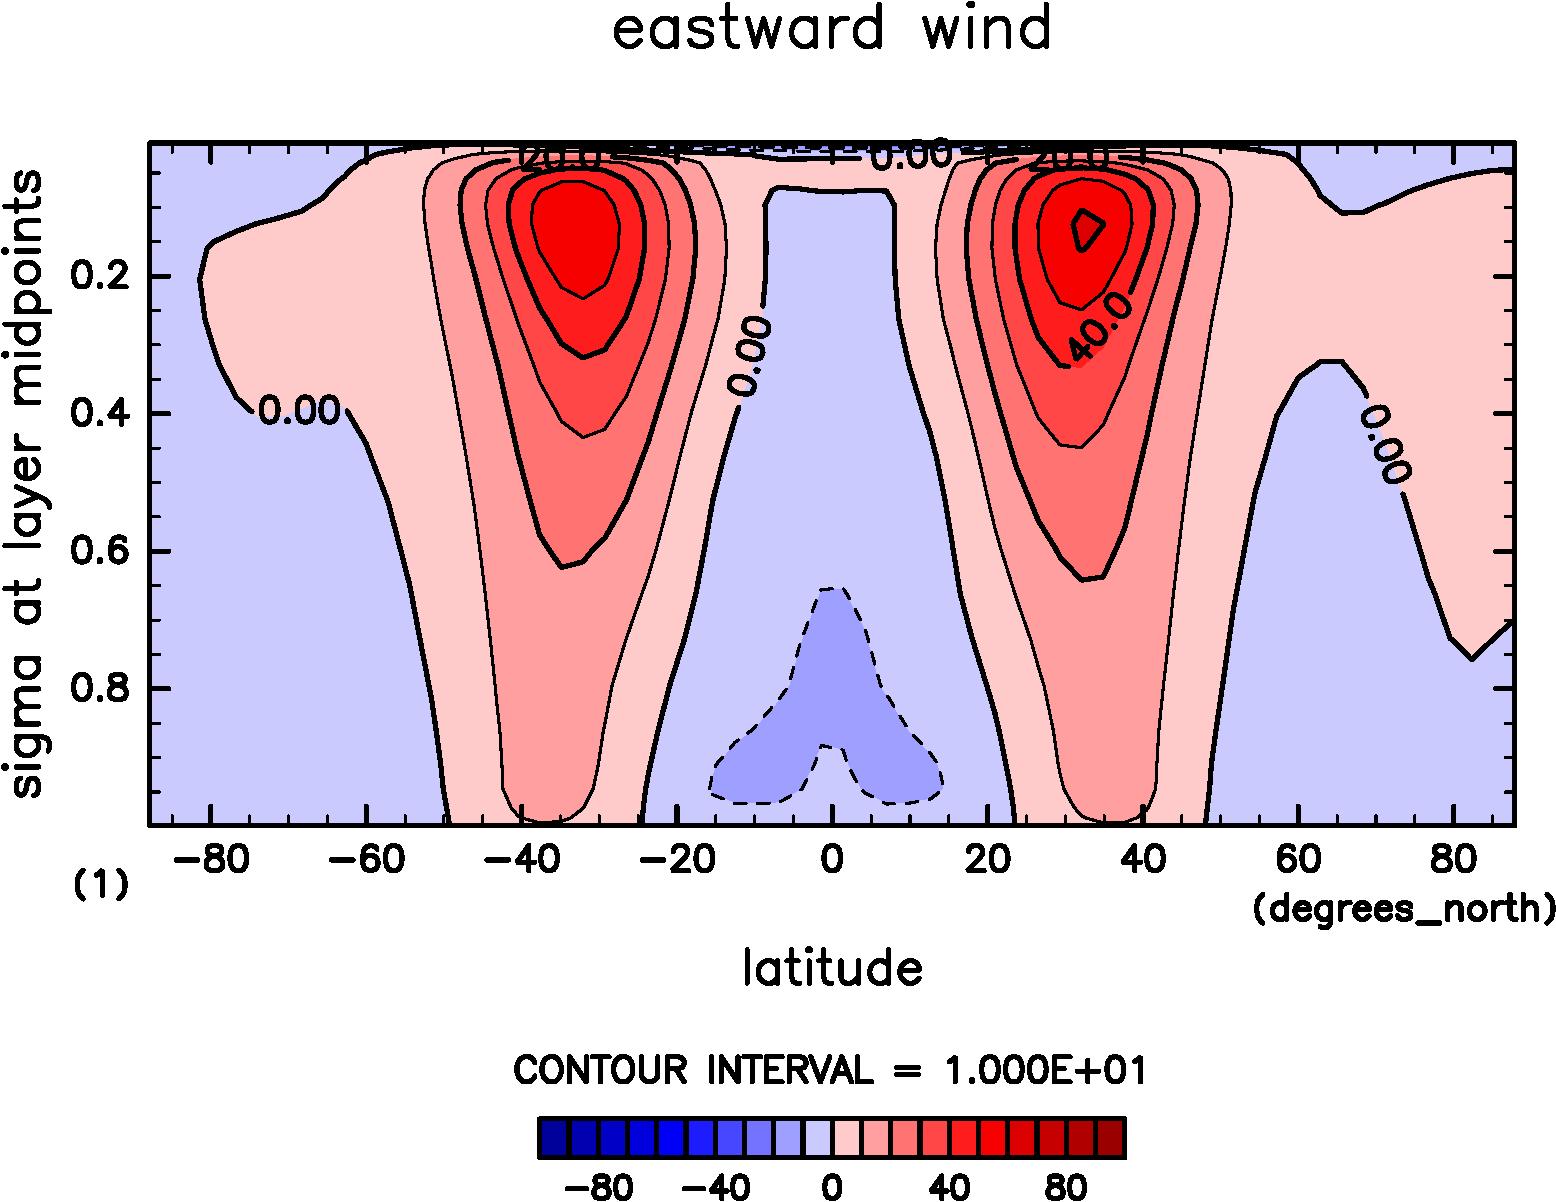
\includegraphics[width=\textwidth]{S1366/U,time=14600:14965-crop-rotate.pdf}
		\caption{東西風\hmu*{[m/s]}}\label{S1366東西風}
	\end{subfigure}
	\begin{subfigure}{.4\textwidth}
		\centering
		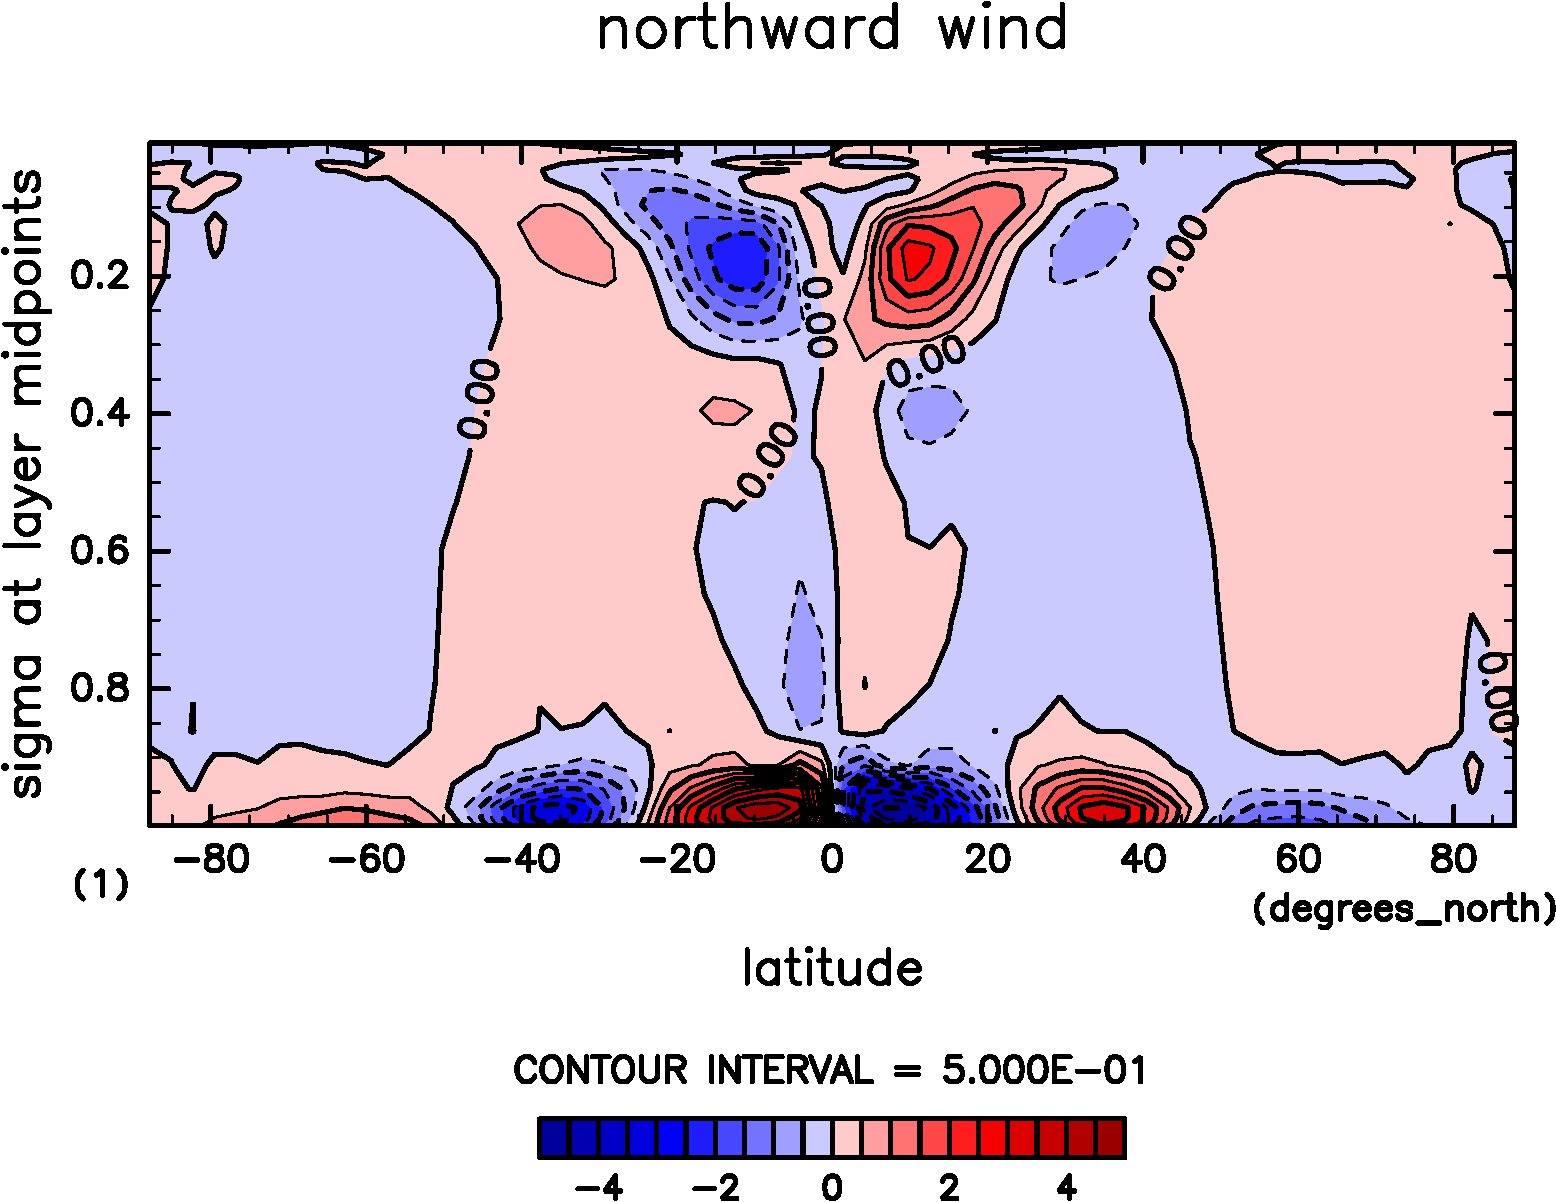
\includegraphics[width=\textwidth]{S1366/V,time=14600:14965-crop-rotate.pdf}
		\caption{南北風\hmu*{[m/s]}}\label{S1366南北風}
	\end{subfigure}
	\begin{subfigure}{.4\textwidth}
		\centering
		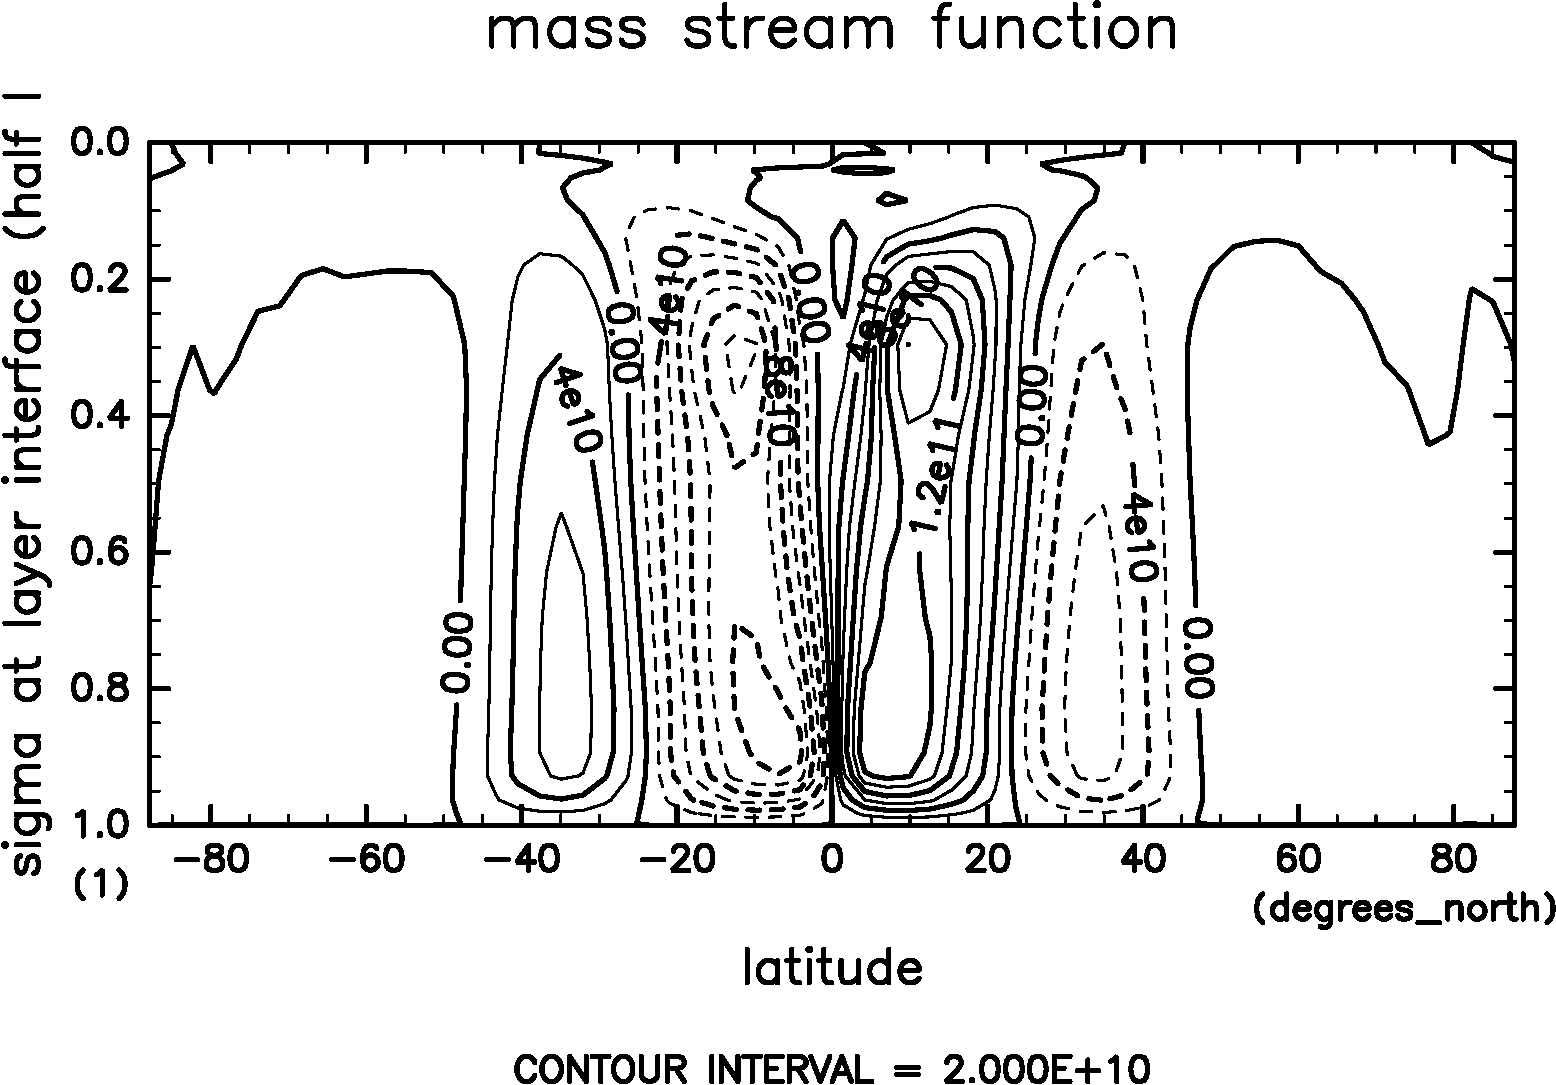
\includegraphics[width=\textwidth,]{S1366/MSF,time=14600:14965-crop-rotate.pdf}
		\\\vspace{13pt}
		\caption{質量流線関数\hmu*{[kg/s]}}\label{S1366質量流線関数}
	\end{subfigure}
	\begin{subfigure}{.4\textwidth}
		\centering
		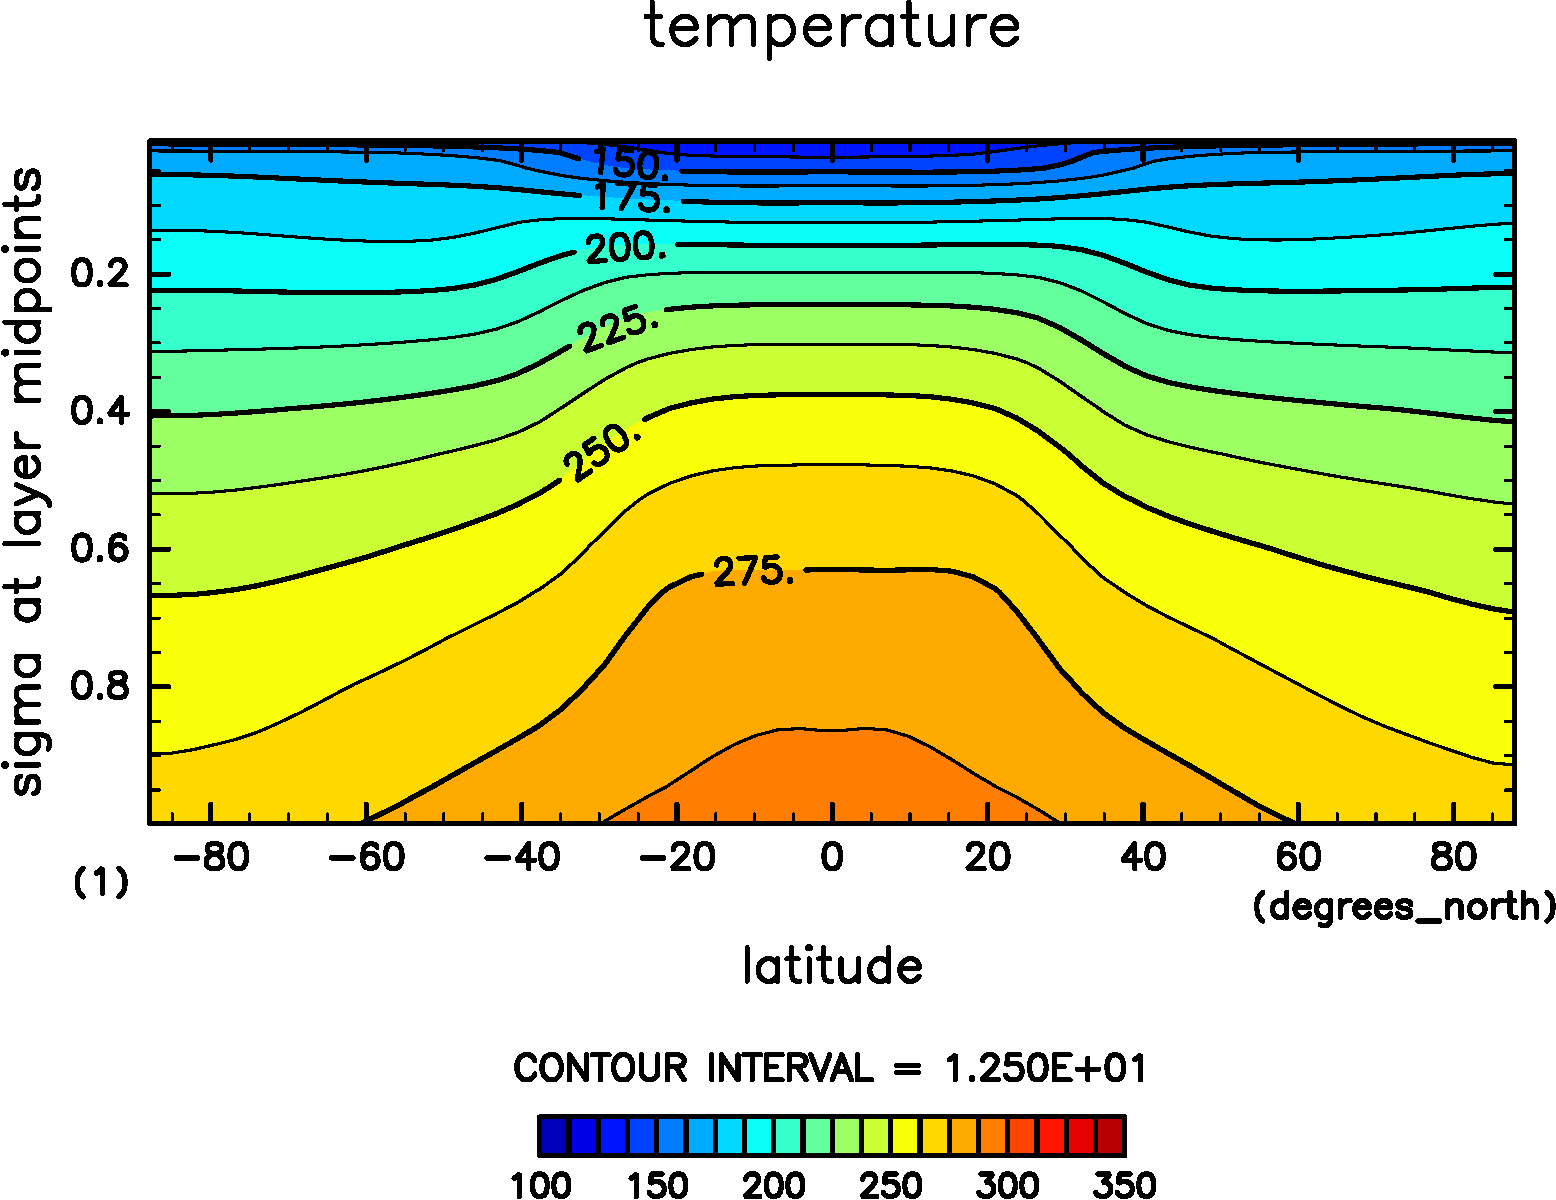
\includegraphics[width=\textwidth]{S1366/Temp,time=14600:14965-crop-rotate.pdf}
		\caption{気温\hmu*{[K]}}\label{S1366気温分布}
	\end{subfigure}
	\begin{subfigure}{.4\textwidth}
		\centering
		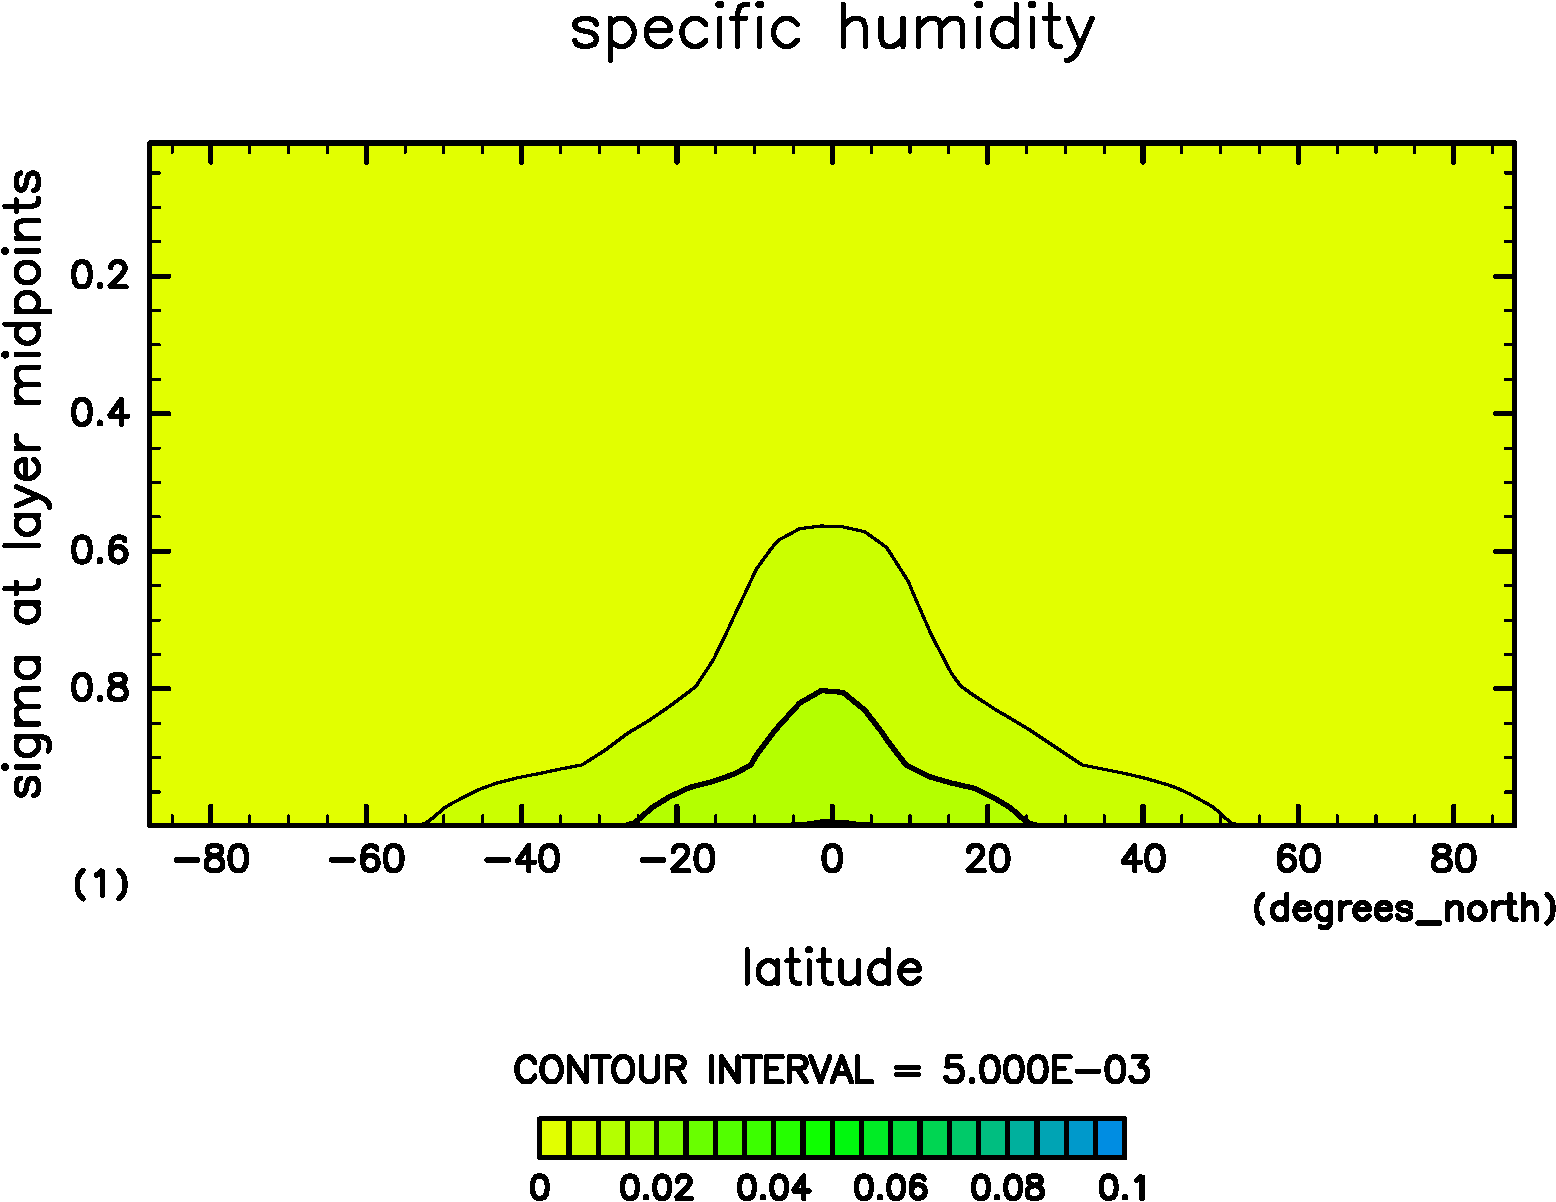
\includegraphics[width=\textwidth]{S1366/QH2OVap,time=14600:14965-crop-rotate.pdf}
		\caption{比湿\hmu*{[kg/kg]}}\label{S1366比湿}
	\end{subfigure}
	\begin{subfigure}{.4\textwidth}
		\centering
		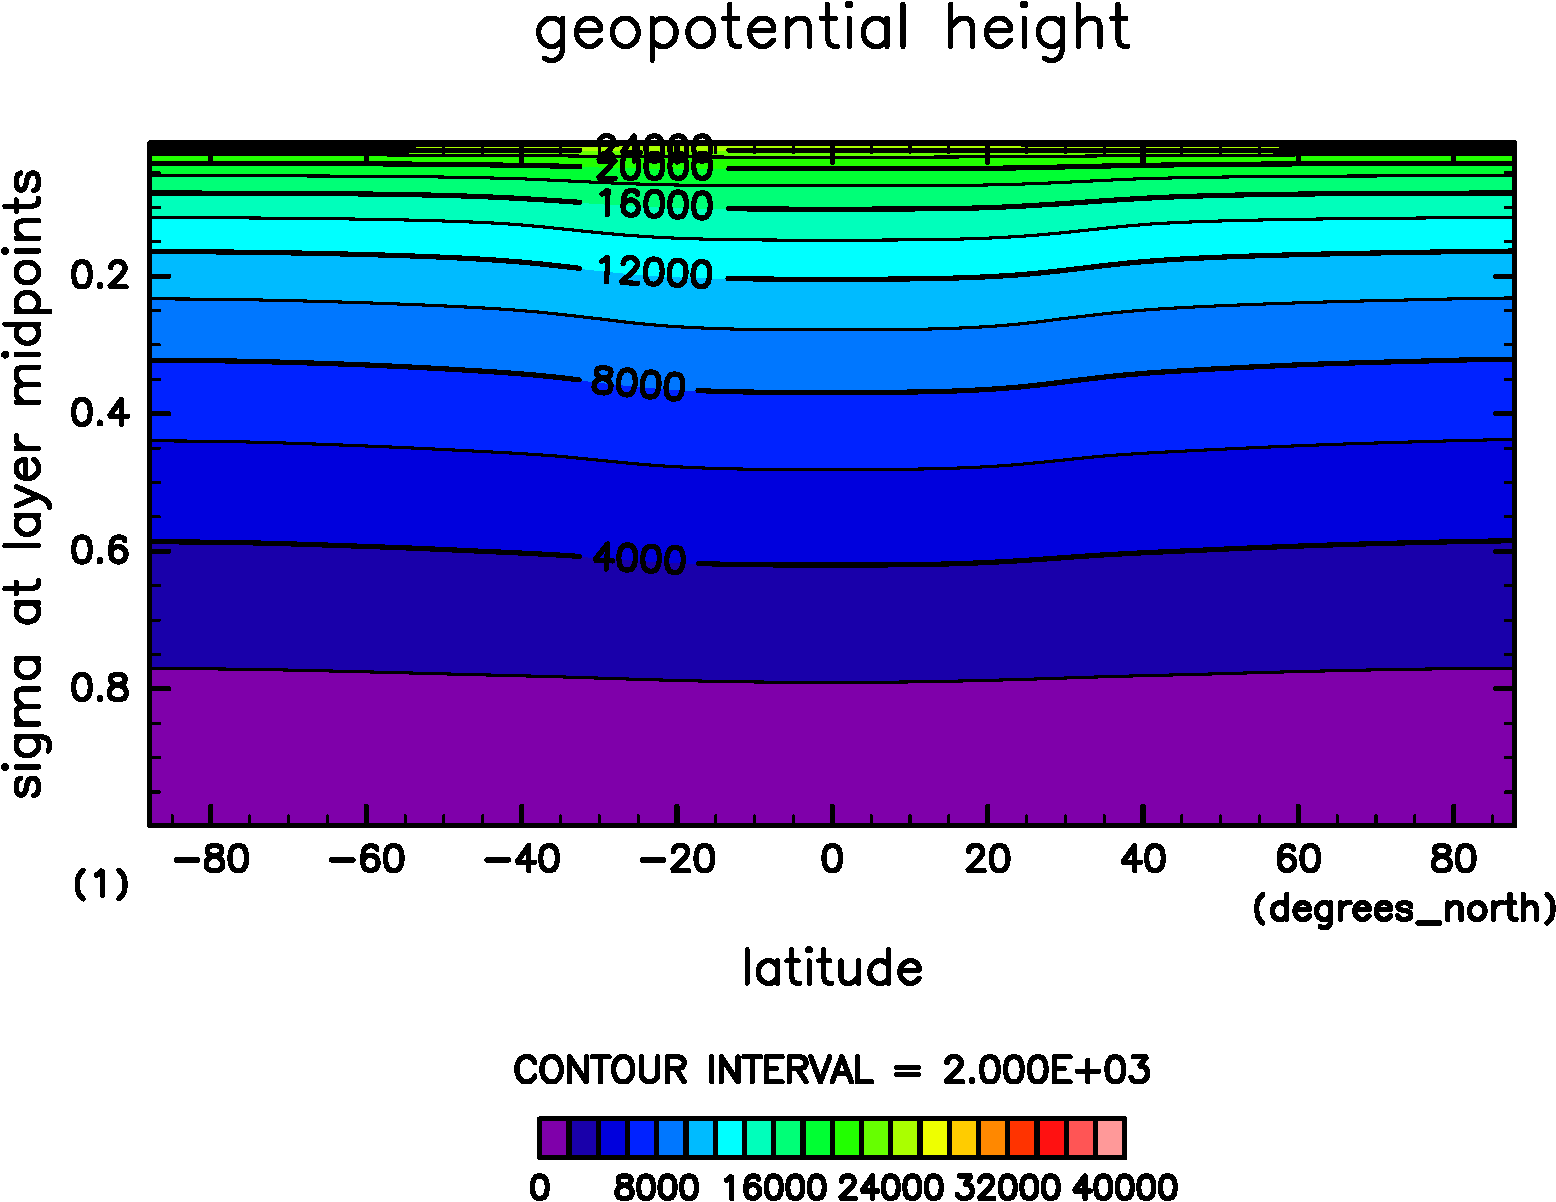
\includegraphics[width=\textwidth]{S1366/Height,time=14600:14965-crop-rotate.pdf}
		\caption{ジオポテンシャル高度\hmu*{[m/s]}}\label{S1366ジオポテンシャル高度}
	\end{subfigure}
	\caption[実験 S1366 の各物理量の子午面分布]{
		実験 S1366 の各物理量の子午面分布。
		いずれも 41 年目の値を緯度平均、時間平均(間隔 0.25 日)した図を示す。
		(\subref{S1366東西風}) 東西風の等値線間隔は \(10\hmu{m/s}\)、
		(\subref{S1366南北風}) 南北風の等値線間隔は \(0.5\hmu{m/s}\)、
		(\subref{S1500質量流線関数}) 質量流線関数の等値線間隔は \(2\hme{-10}\hmu{kg/s}\)、
		(\subref{S1366気温分布}) 気温分布の等値線間隔は \(12.5\hmu{K}\)、
		(\subref{S1366比湿}) 比湿の等値線間隔は \(5\hme{-3}\hmu{kg/kg}\)、
		(\subref{S1366ジオポテンシャル高度}) ジオポテンシャル高度の等値線間隔は \(2000\hmu{m}\) である。
	}\label{S1366}
\end{figure}

\begin{figure}[t]
	\centering
	\begin{subfigure}{.4\textwidth}
		\centering
		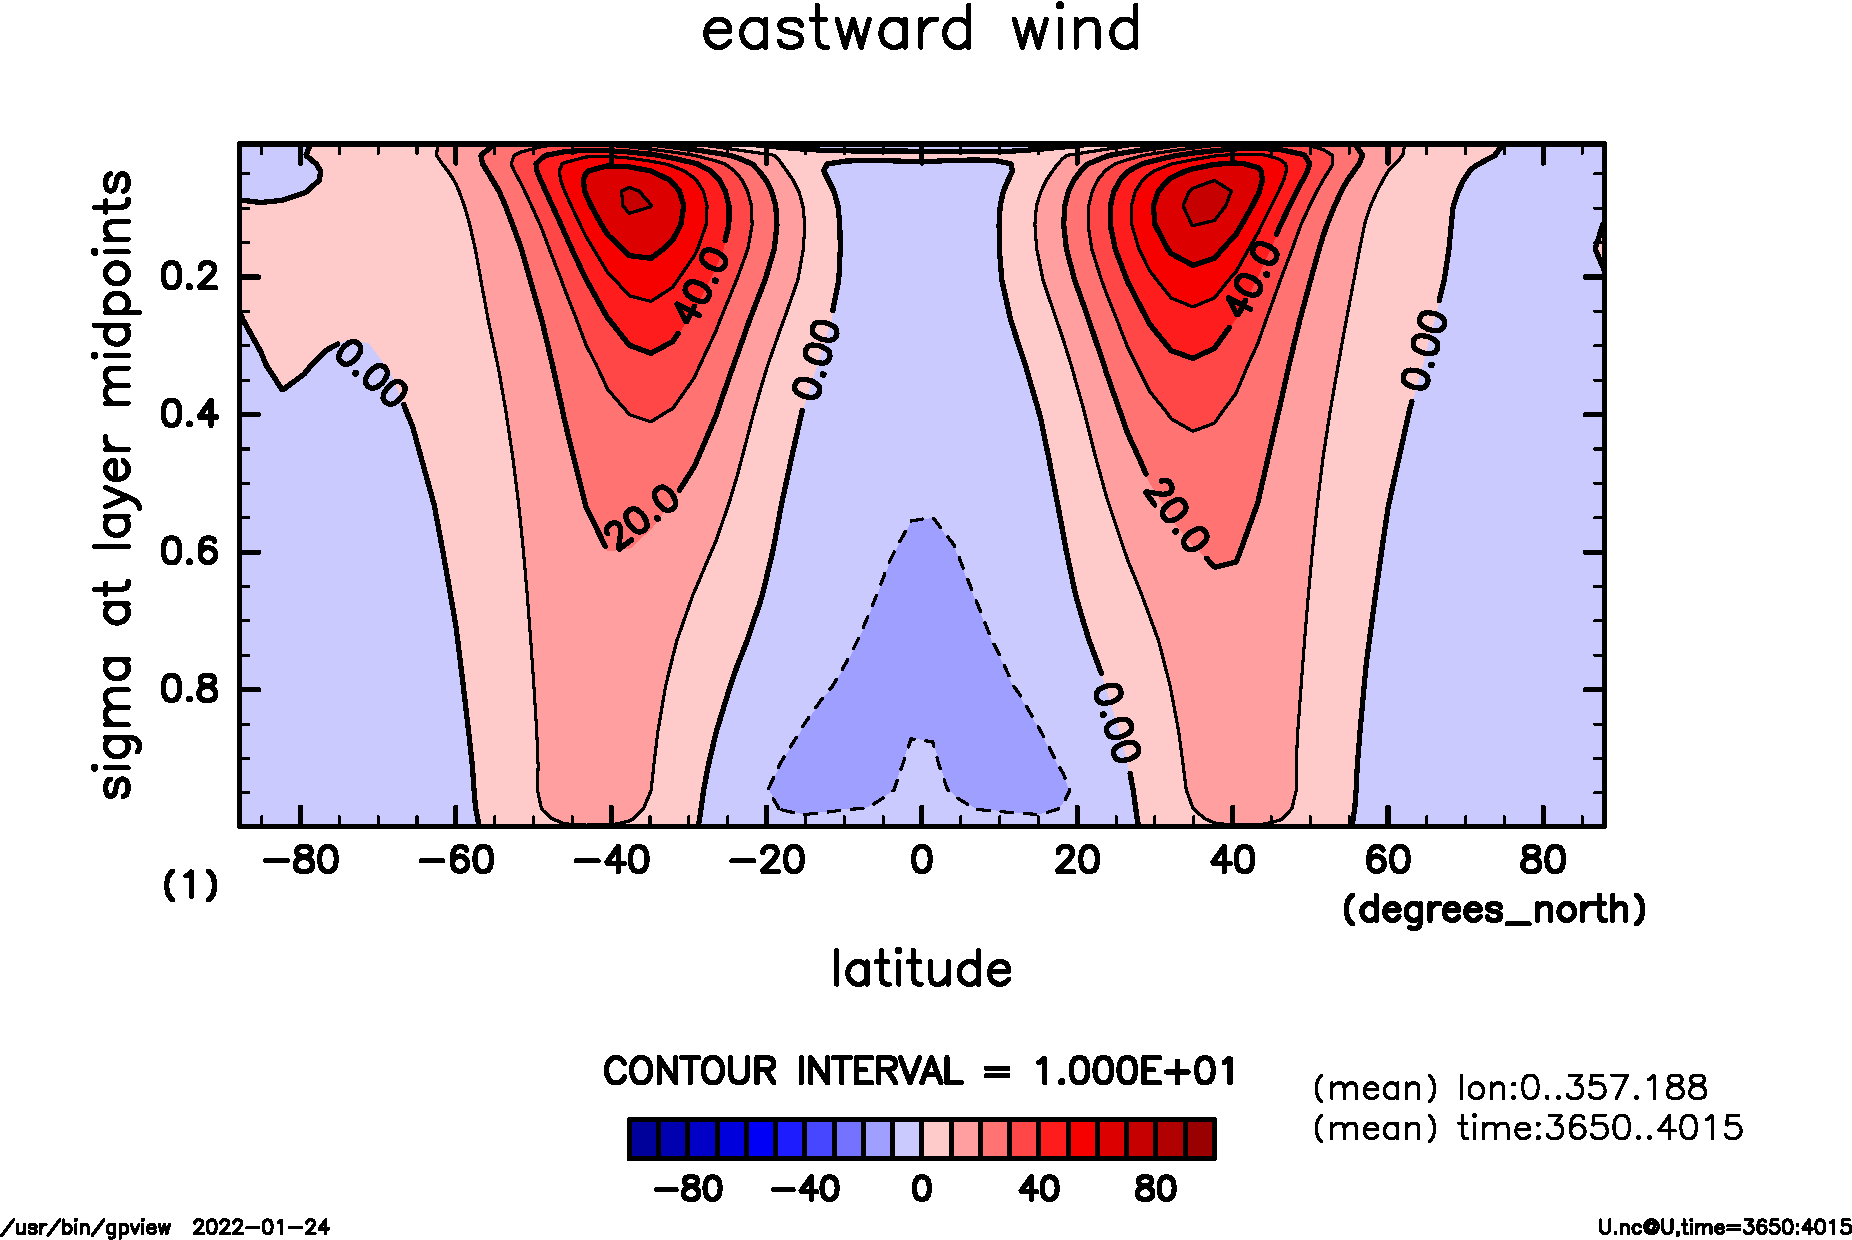
\includegraphics[width=\textwidth]{S1500/U,time=3650:4015-crop-rotate.pdf}
		\caption{東西風\hmu*{[m/s]}}\label{S1500東西風}
	\end{subfigure}
	\begin{subfigure}{.4\textwidth}
		\centering
		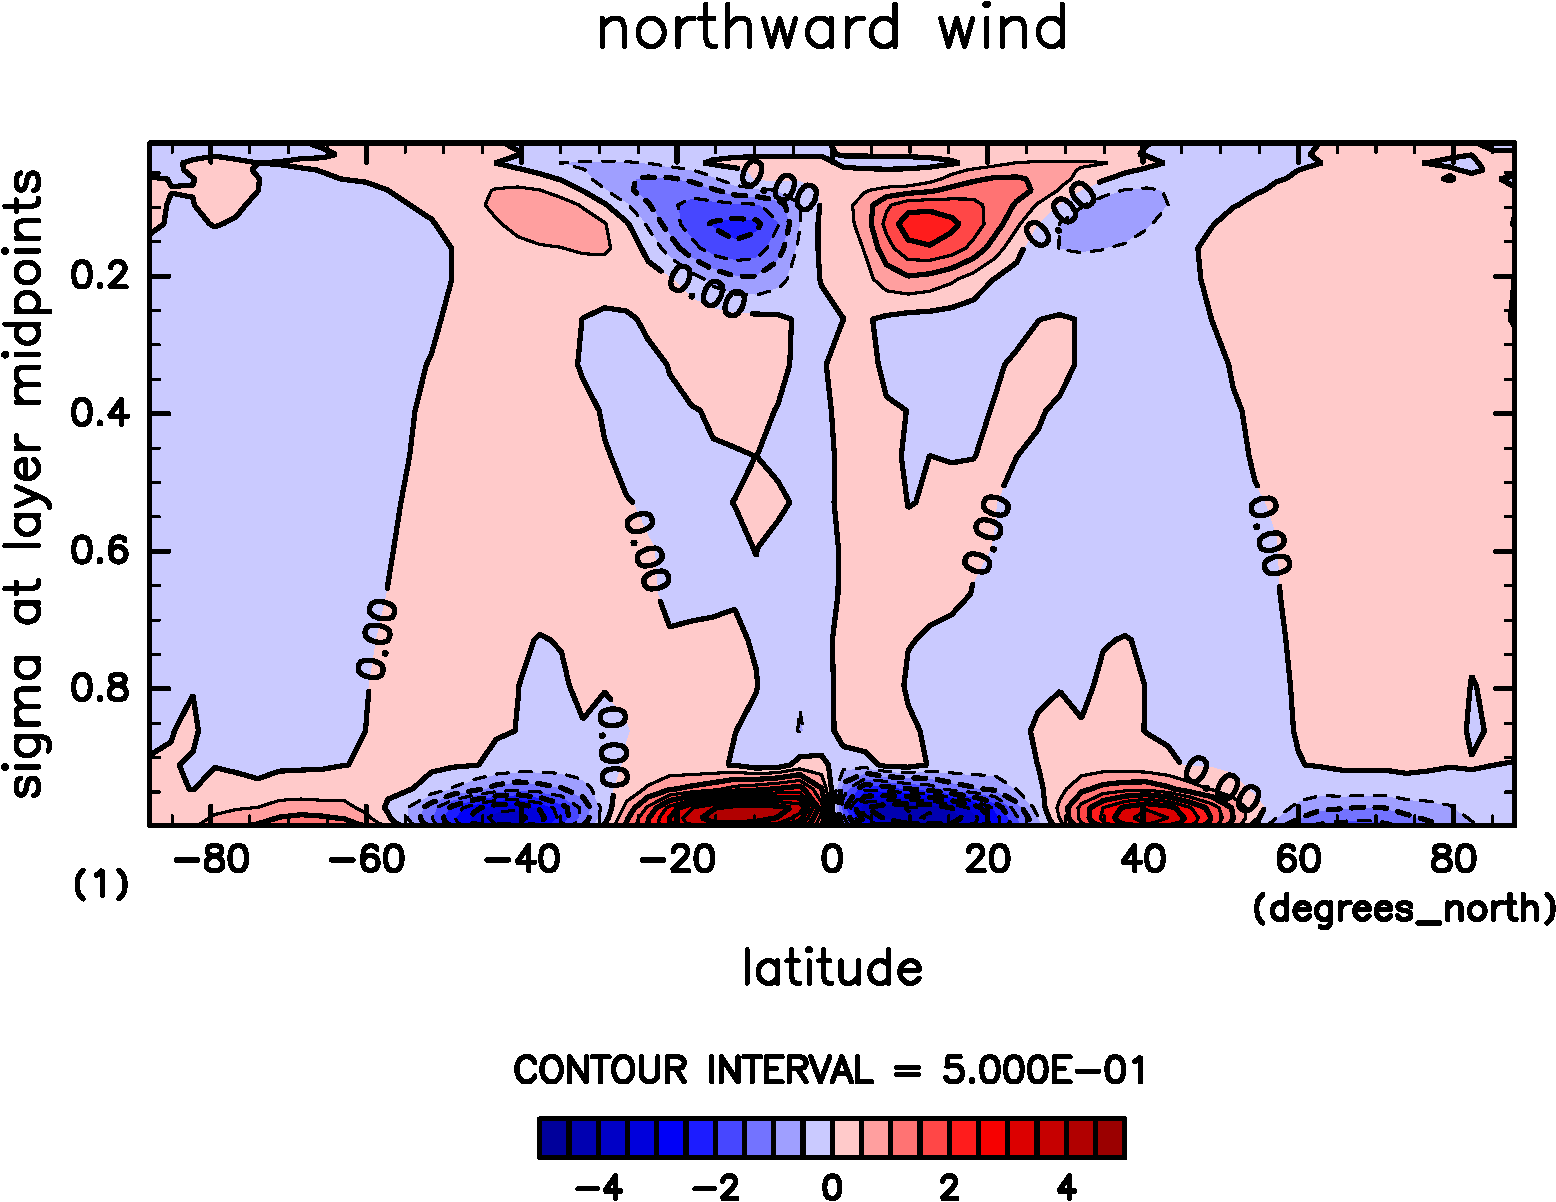
\includegraphics[width=\textwidth]{S1500/V,time=3650:4015-crop-rotate.pdf}
		\caption{南北風\hmu*{[m/s]}}\label{S1500南北風}
	\end{subfigure}
	\begin{subfigure}{.4\textwidth}
		\centering
		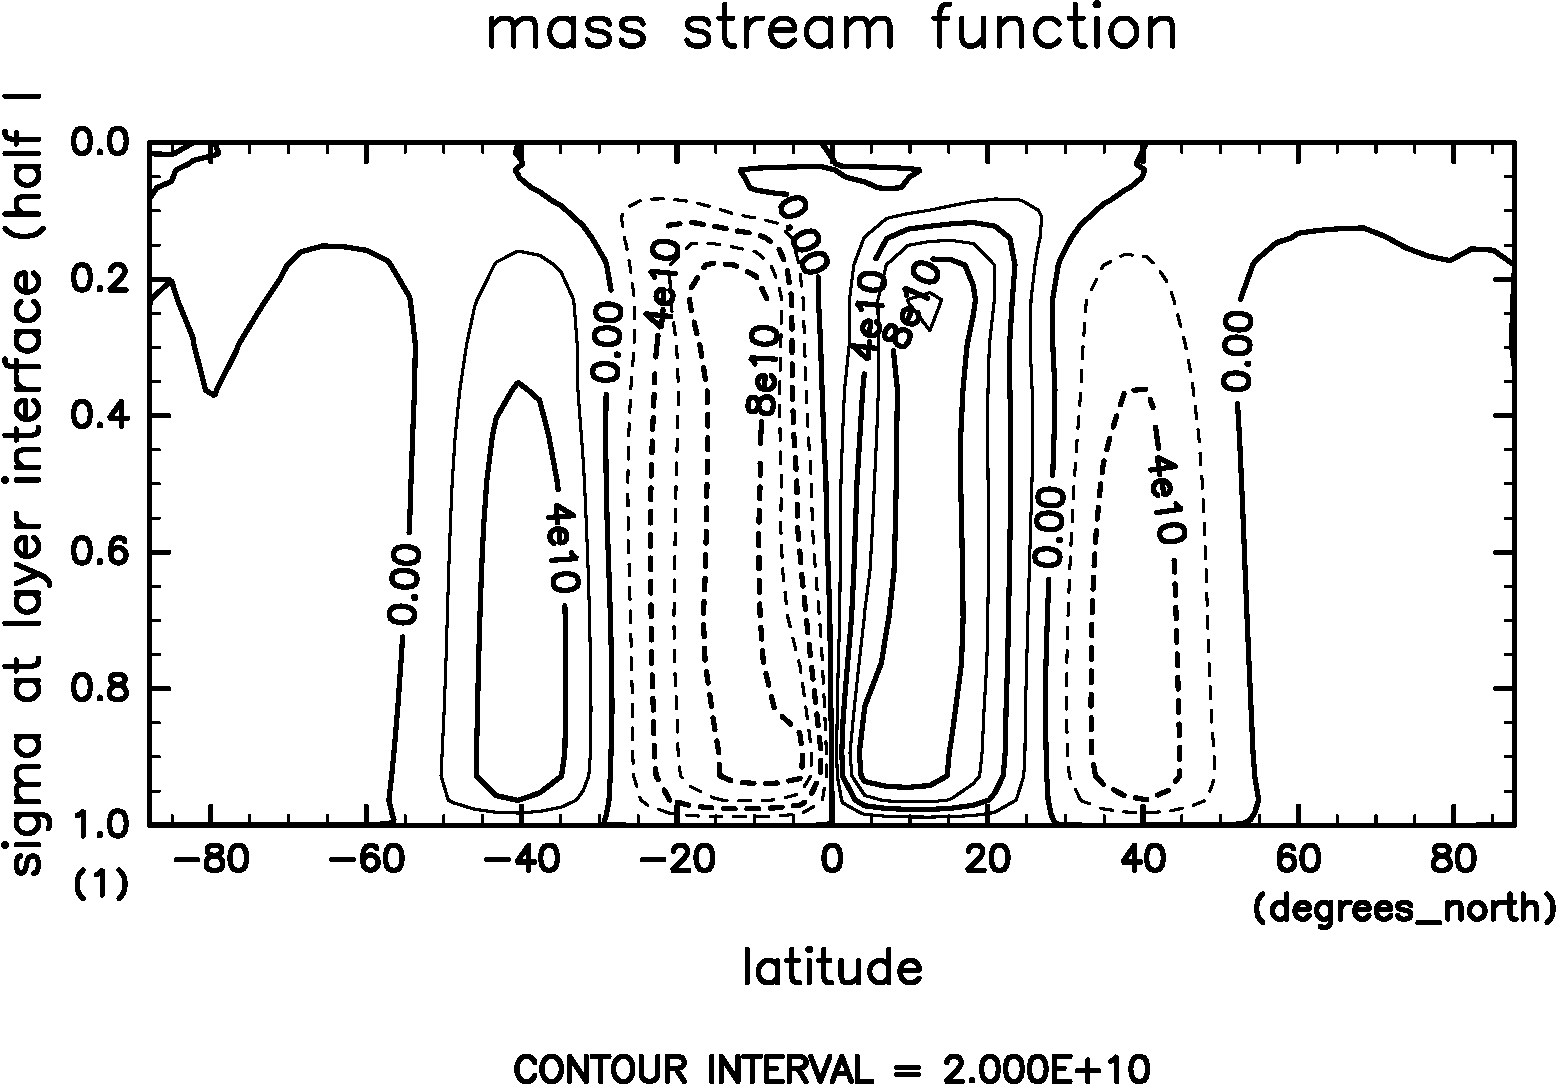
\includegraphics[width=\textwidth]{S1500/MSF,time=3650:4015-crop-rotate.pdf}
		\\\vspace{13pt}
		\caption{質量流線関数\hmu*{[kg/s]}}\label{S1500質量流線関数}
	\end{subfigure}
	\begin{subfigure}{.4\textwidth}
		\centering
		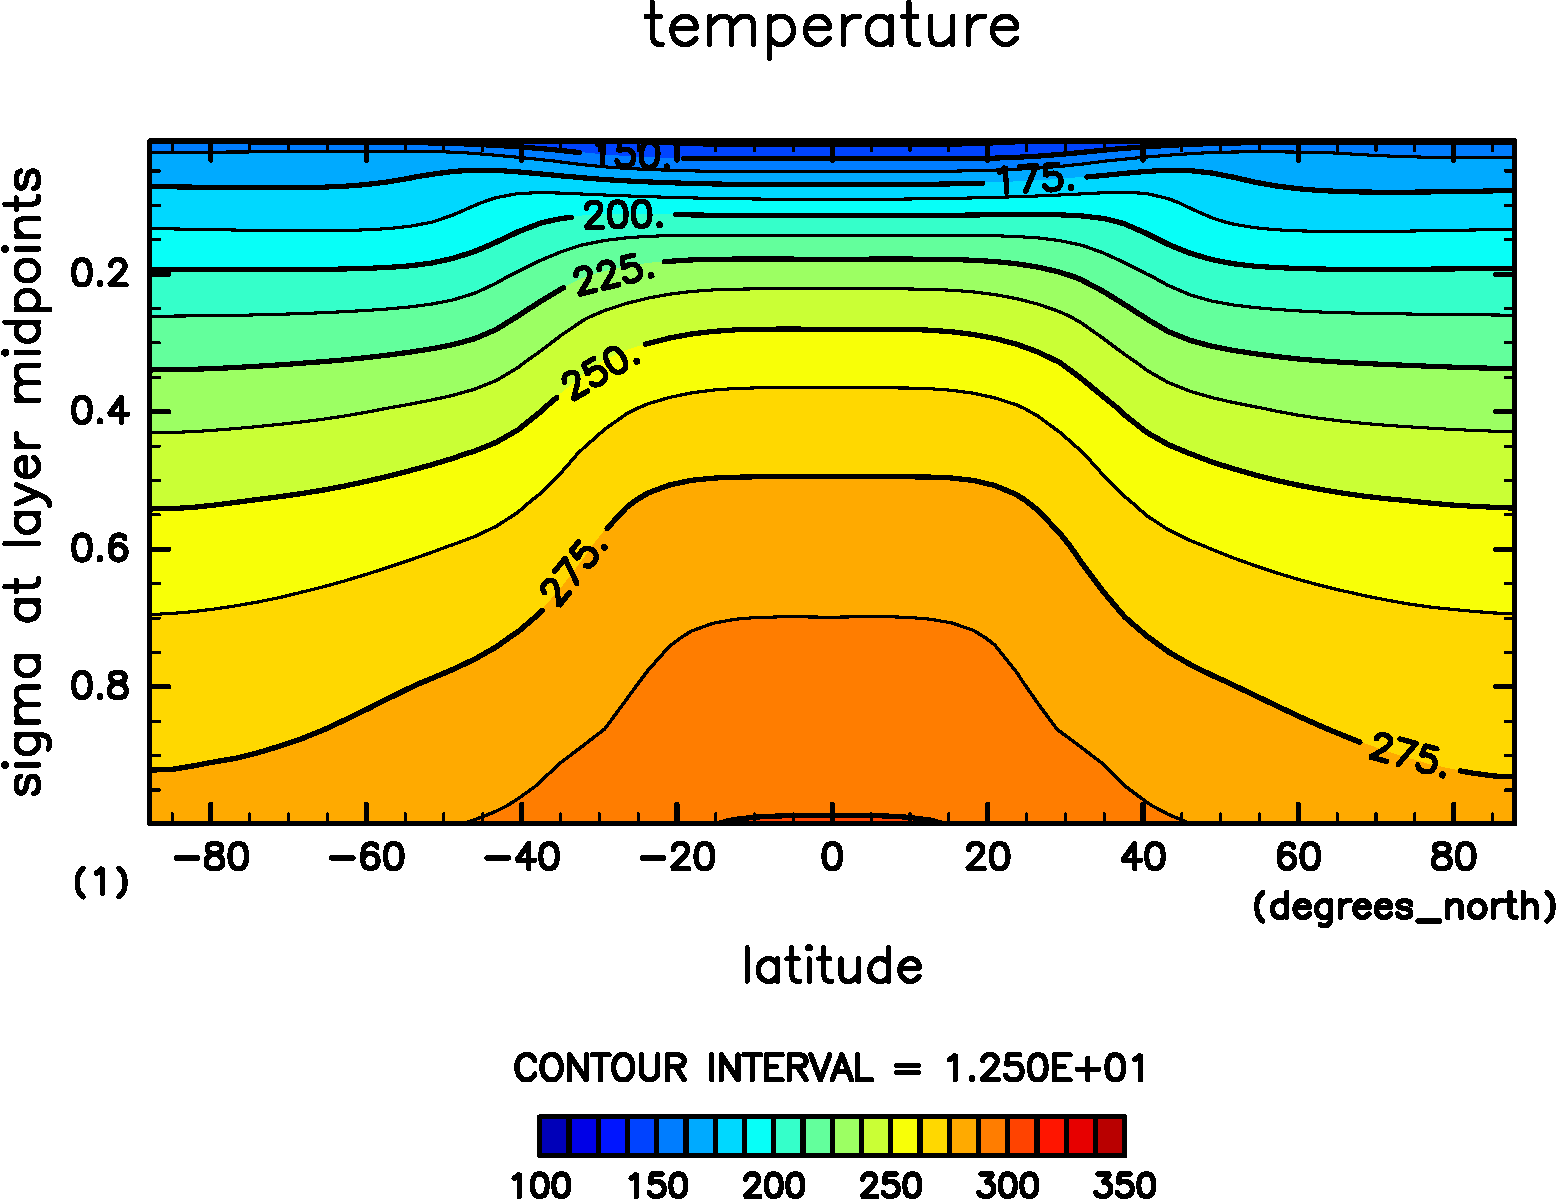
\includegraphics[width=\textwidth]{S1500/Temp,time=3650:4015-crop-rotate.pdf}
		\caption{気温\hmu*{[K]}}\label{S1500気温分布}
	\end{subfigure}
	\begin{subfigure}{.4\textwidth}
		\centering
		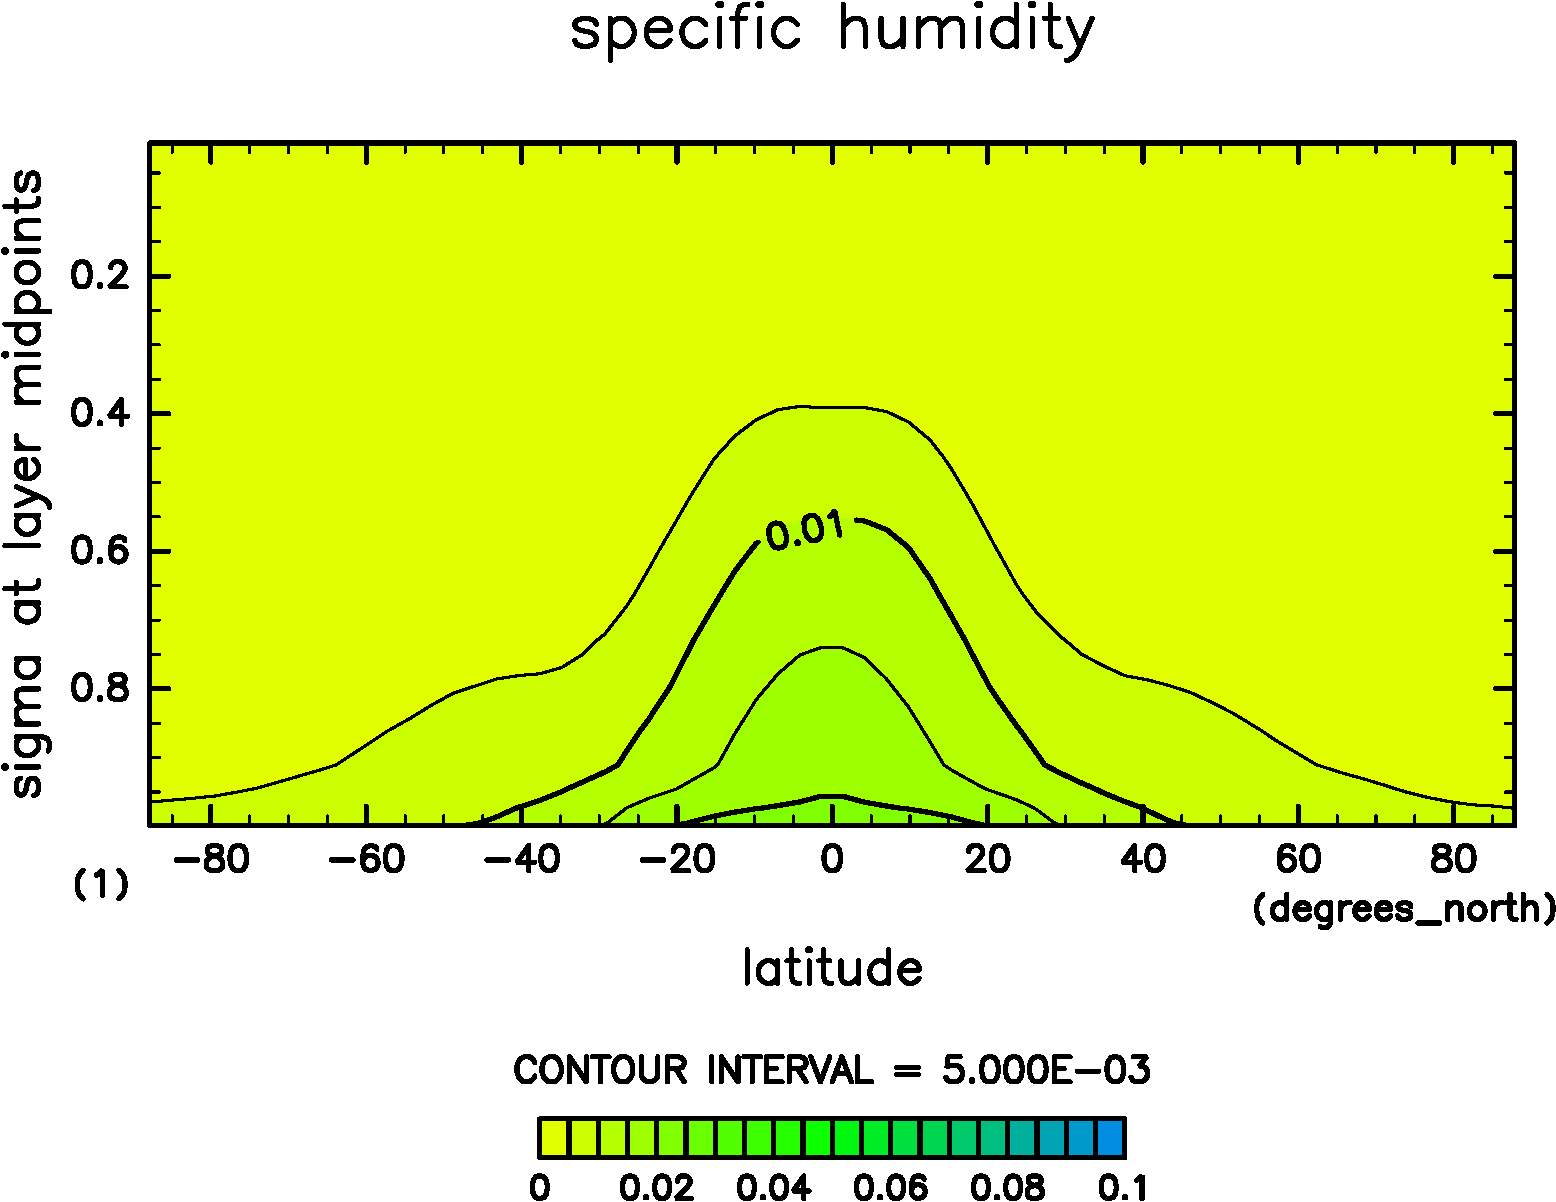
\includegraphics[width=\textwidth]{S1500/QH2OVap,time=3650:4015-crop-rotate.pdf}
		\caption{比湿\hmu*{[kg/kg]}}\label{S1500比湿}
	\end{subfigure}
	\begin{subfigure}{.4\textwidth}
		\centering
		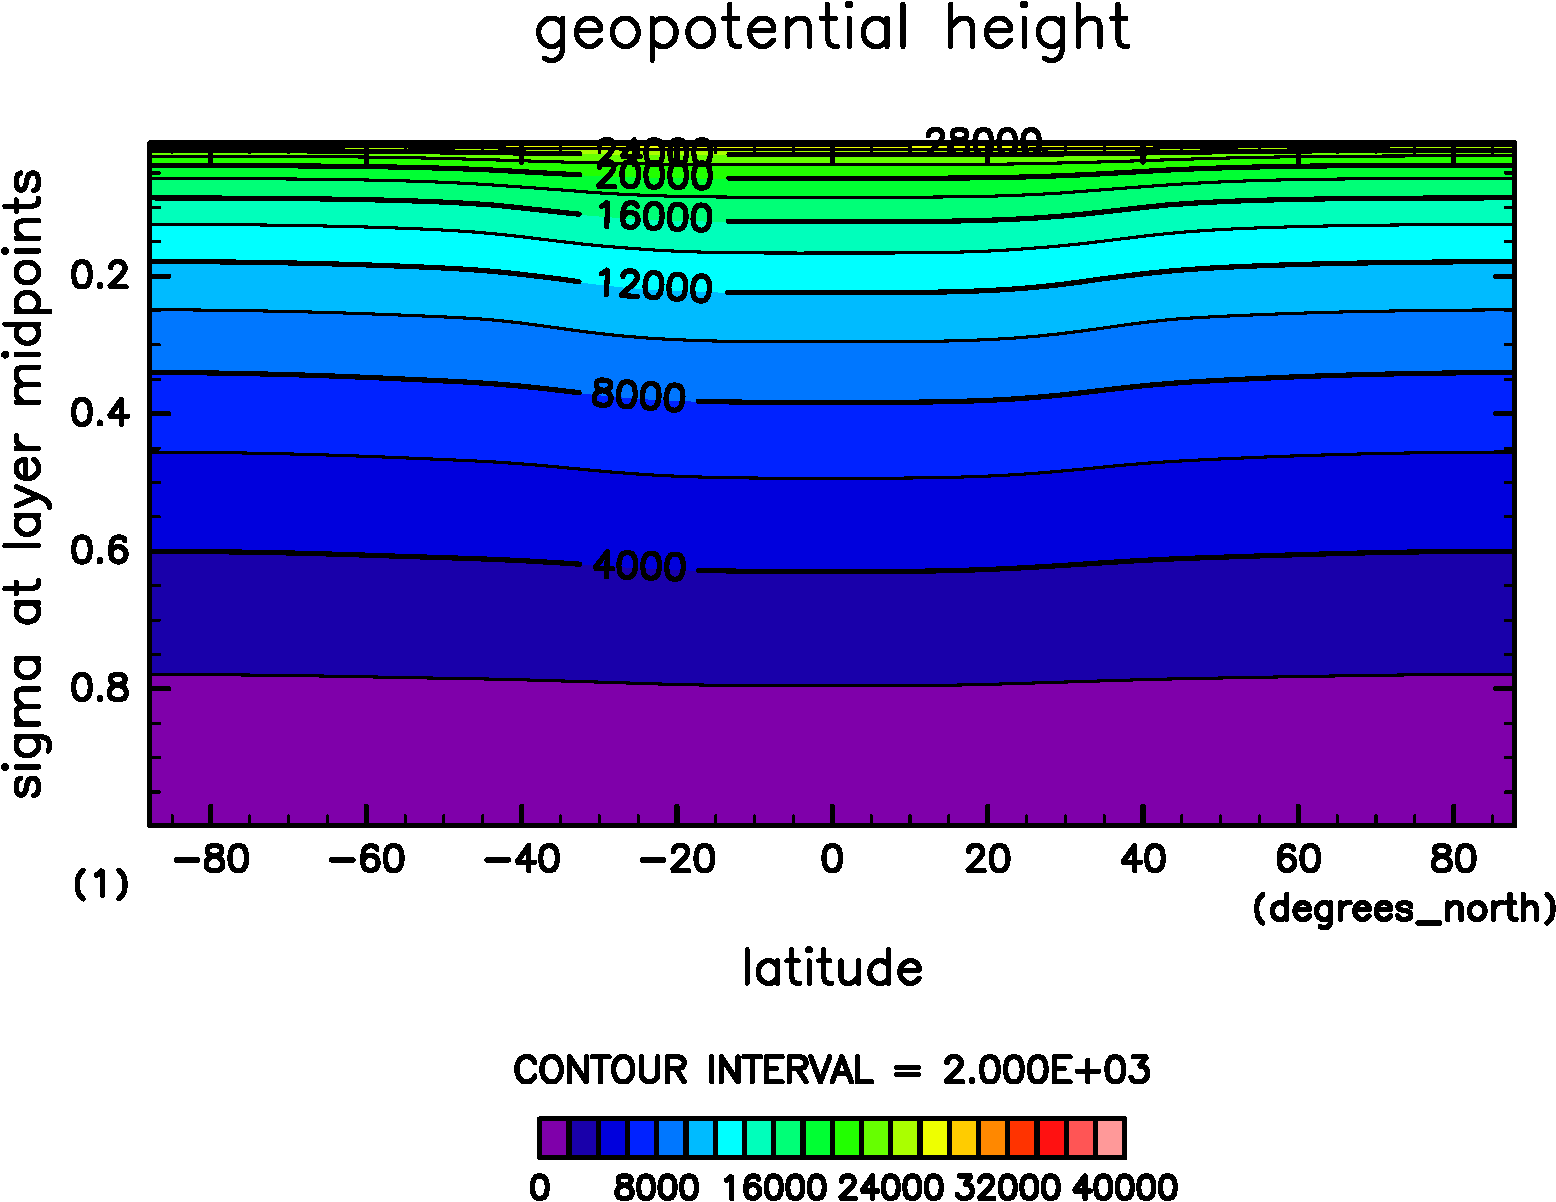
\includegraphics[width=\textwidth]{S1500/Height,time=3650:4015-crop-rotate.pdf}
		\caption{ジオポテンシャル高度\hmu*{[m]}}\label{S1500ジオポテンシャル高度}
	\end{subfigure}
	\caption[実験 S1500 の各物理量の子午面分布]{
		実験 S1500 の各物理量の子午面分布。図 \ref{S1366} と同様の図であるが、
		11 年目の年平均値である。
	}\label{S1500}
\end{figure}

\begin{figure}[t]
	\centering
	\begin{subfigure}{.4\textwidth}
		\centering
		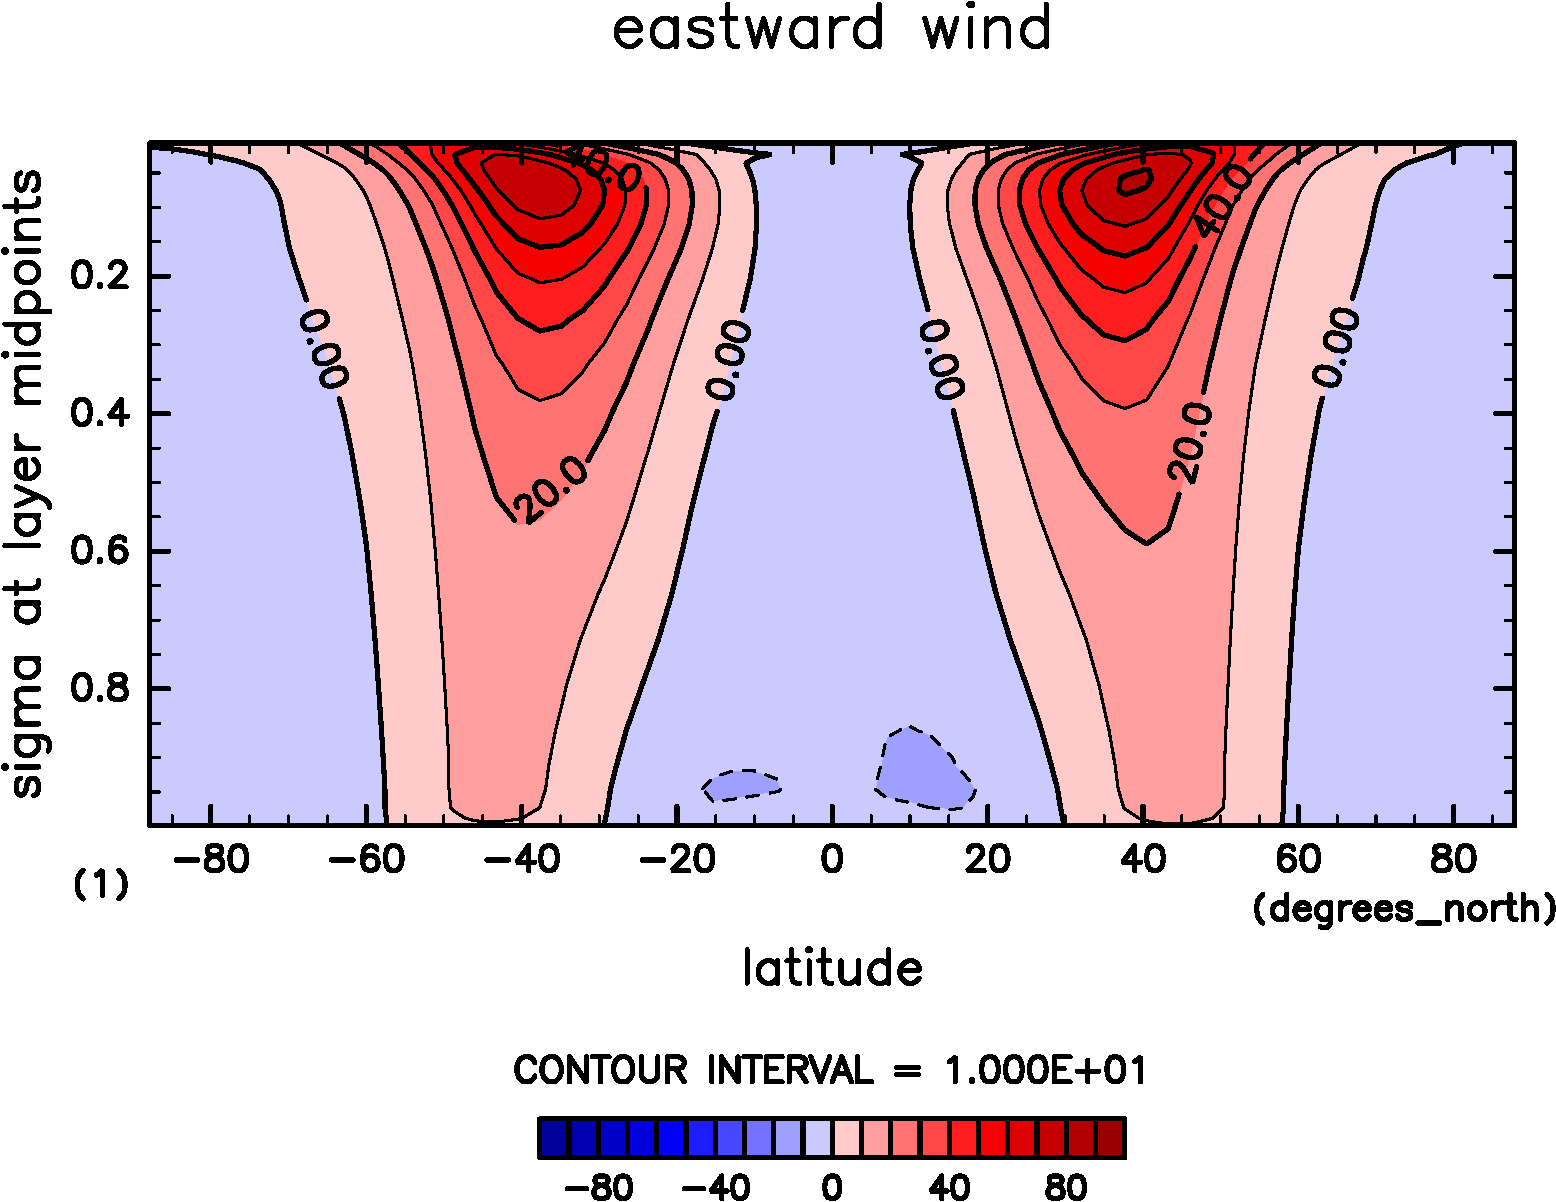
\includegraphics[width=\textwidth]{S1600/U,time=3650:4015-crop-rotate.pdf}
		\caption{東西風\hmu*{[m/s]}}\label{S1600東西風}
	\end{subfigure}
	\begin{subfigure}{.4\textwidth}
		\centering
		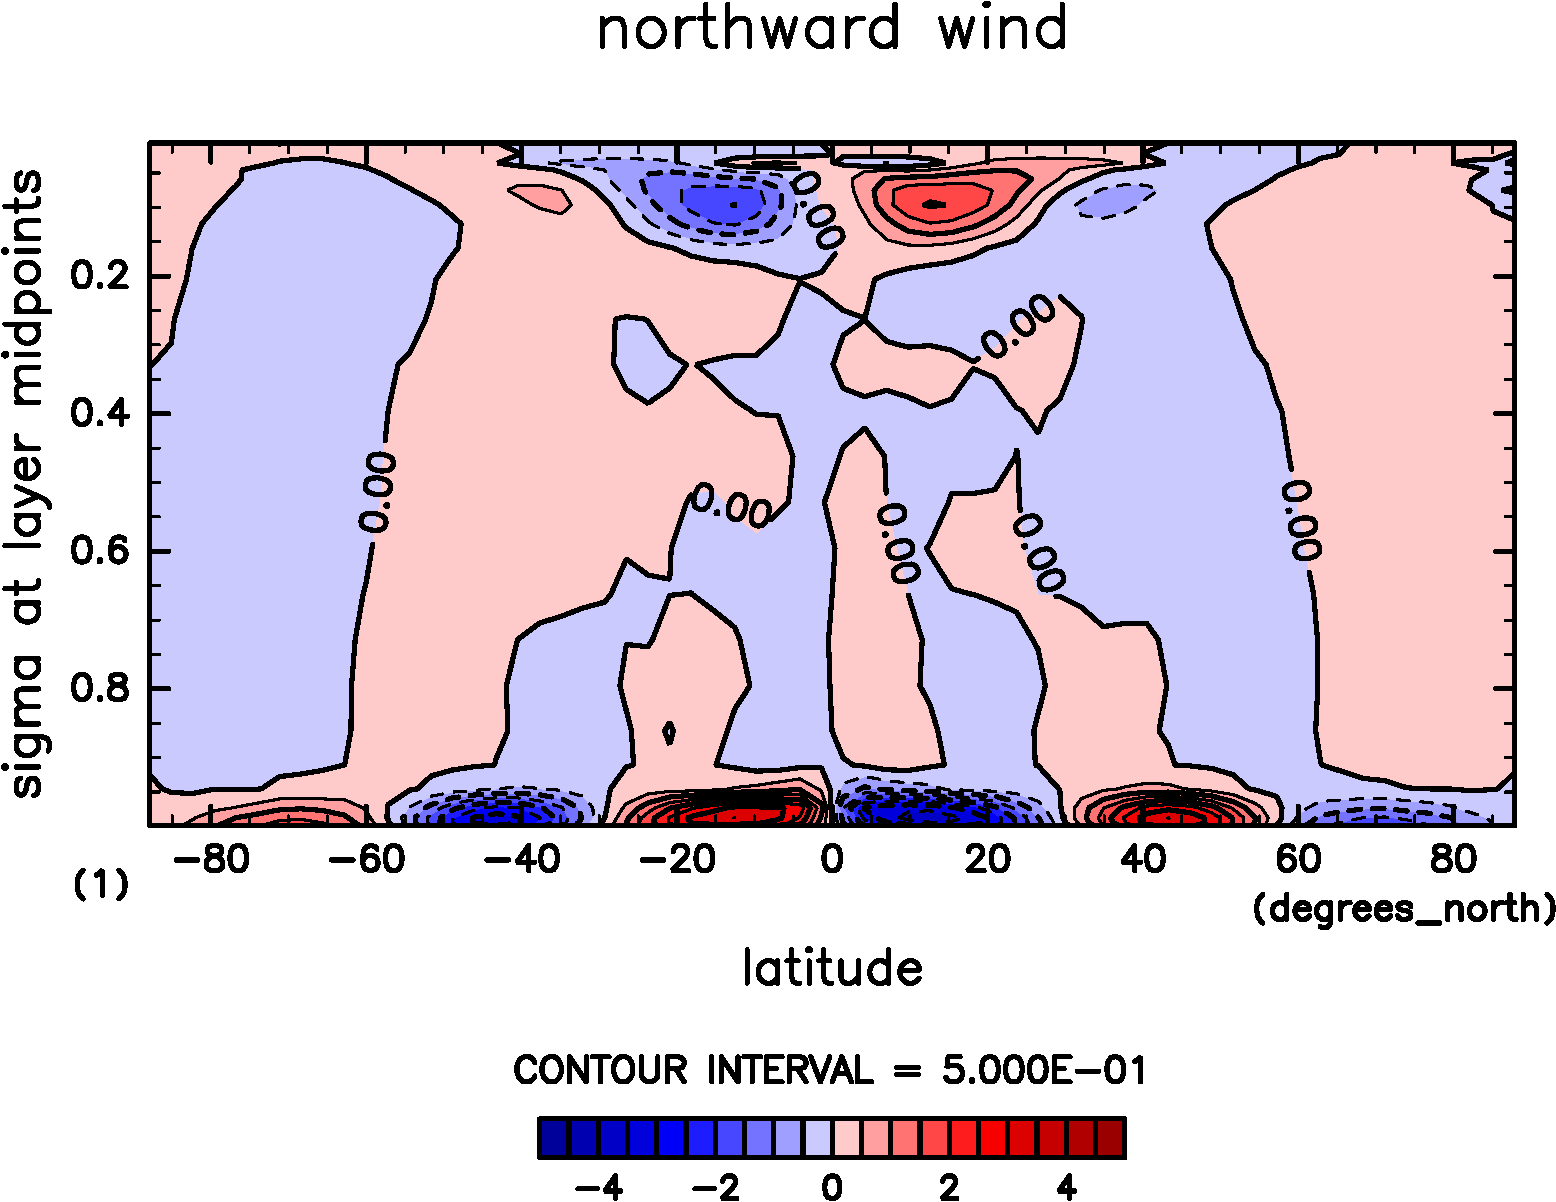
\includegraphics[width=\textwidth]{S1600/V,time=3650:4015-crop-rotate.pdf}
		\caption{南北風\hmu*{[m/s]}}\label{S1600南北風}
	\end{subfigure}
	\begin{subfigure}{.4\textwidth}
		\centering
		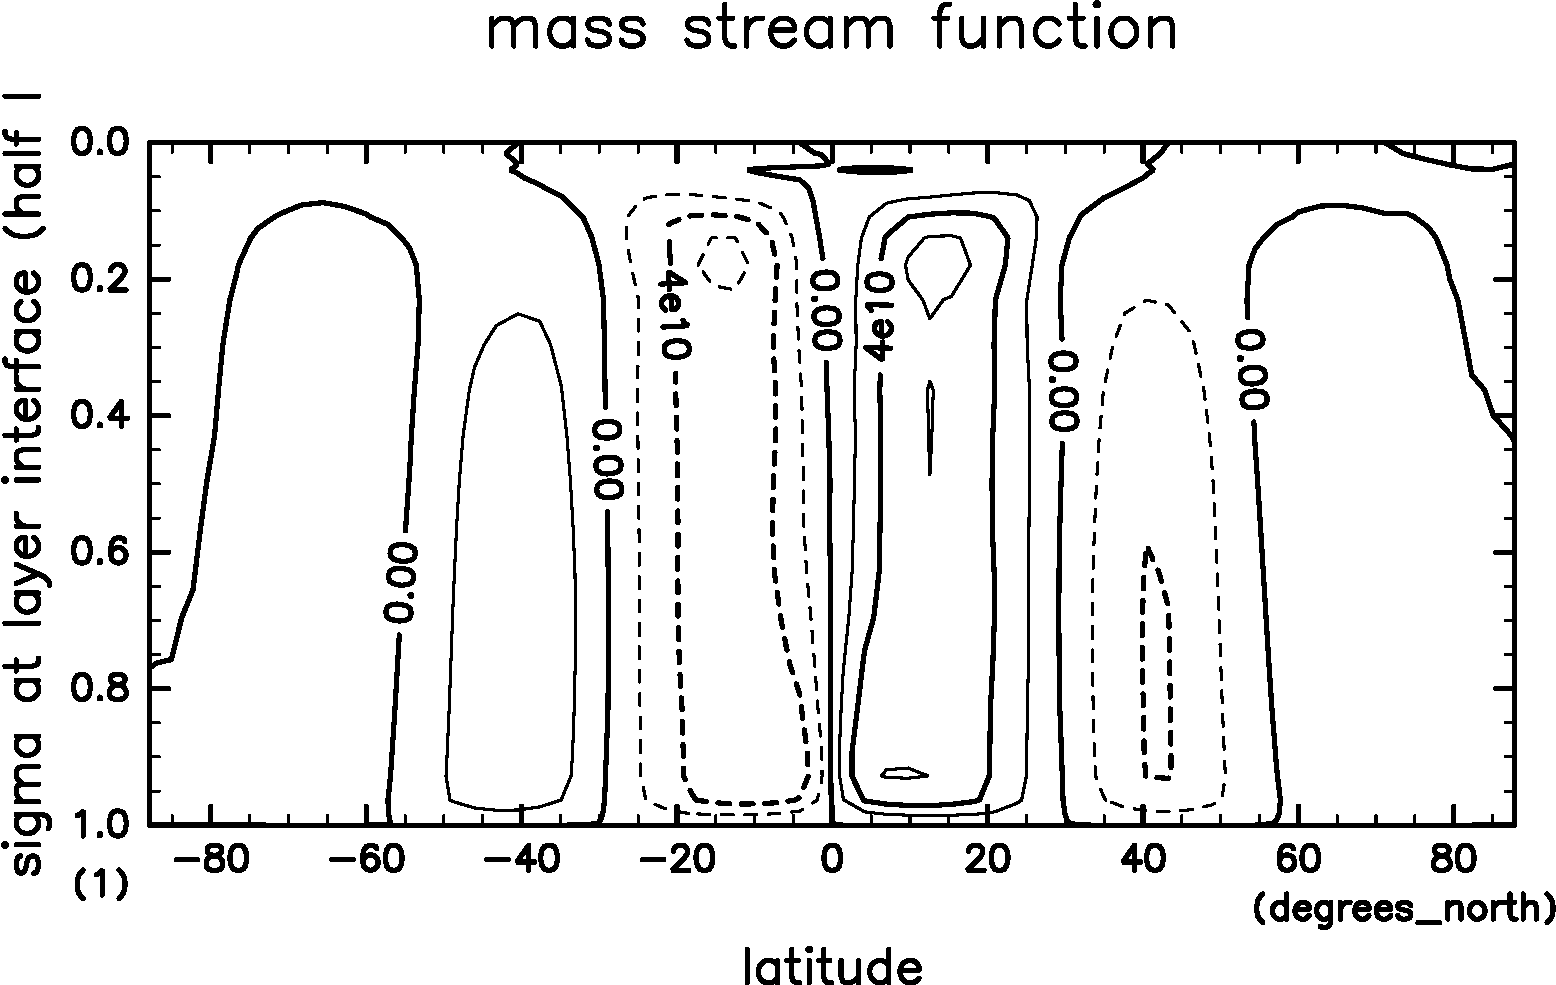
\includegraphics[width=\textwidth]{S1600/MSF,time=3650:4015-crop-rotate.pdf}
		\\\vspace{13pt}
		\caption{質量流線関数\hmu*{[kg/s]}}\label{S1600質量流線関数}
	\end{subfigure}
	\begin{subfigure}{.4\textwidth}
		\centering
		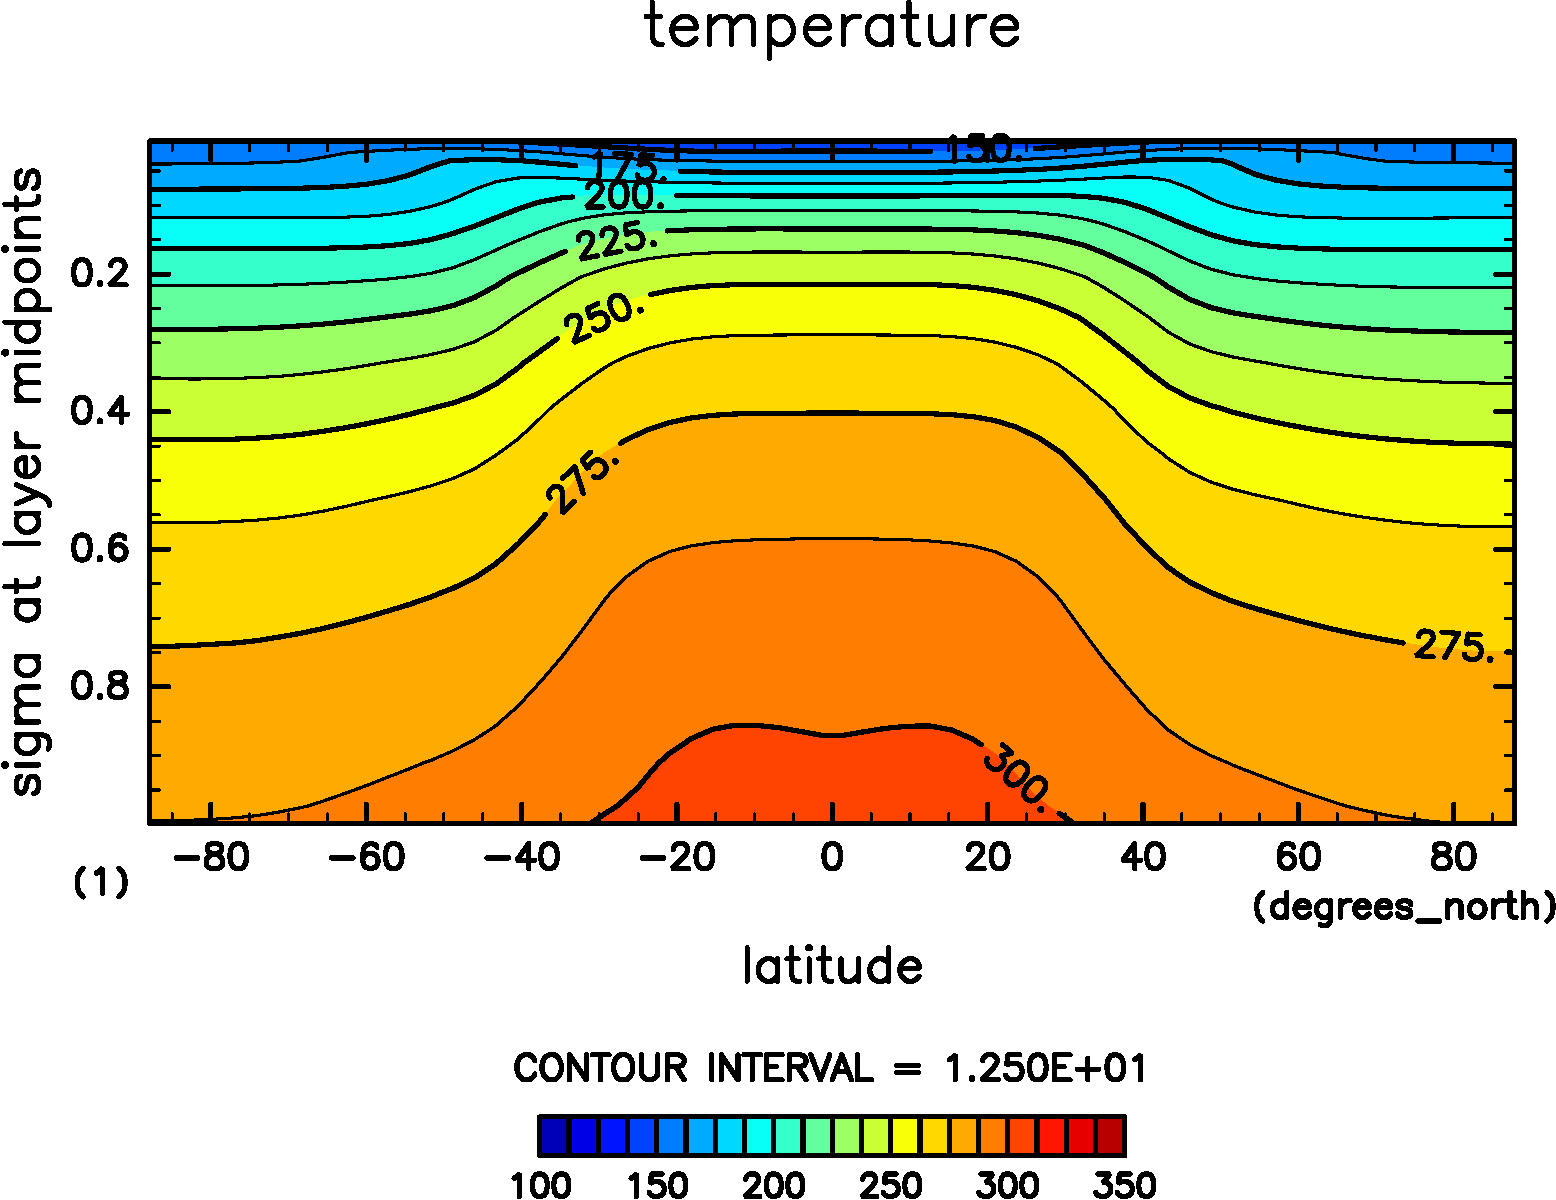
\includegraphics[width=\textwidth]{S1600/Temp,time=3650:4015-crop-rotate.pdf}
		\caption{気温\hmu*{[K]}}\label{S1600気温分布}
	\end{subfigure}
	\begin{subfigure}{.4\textwidth}
		\centering
		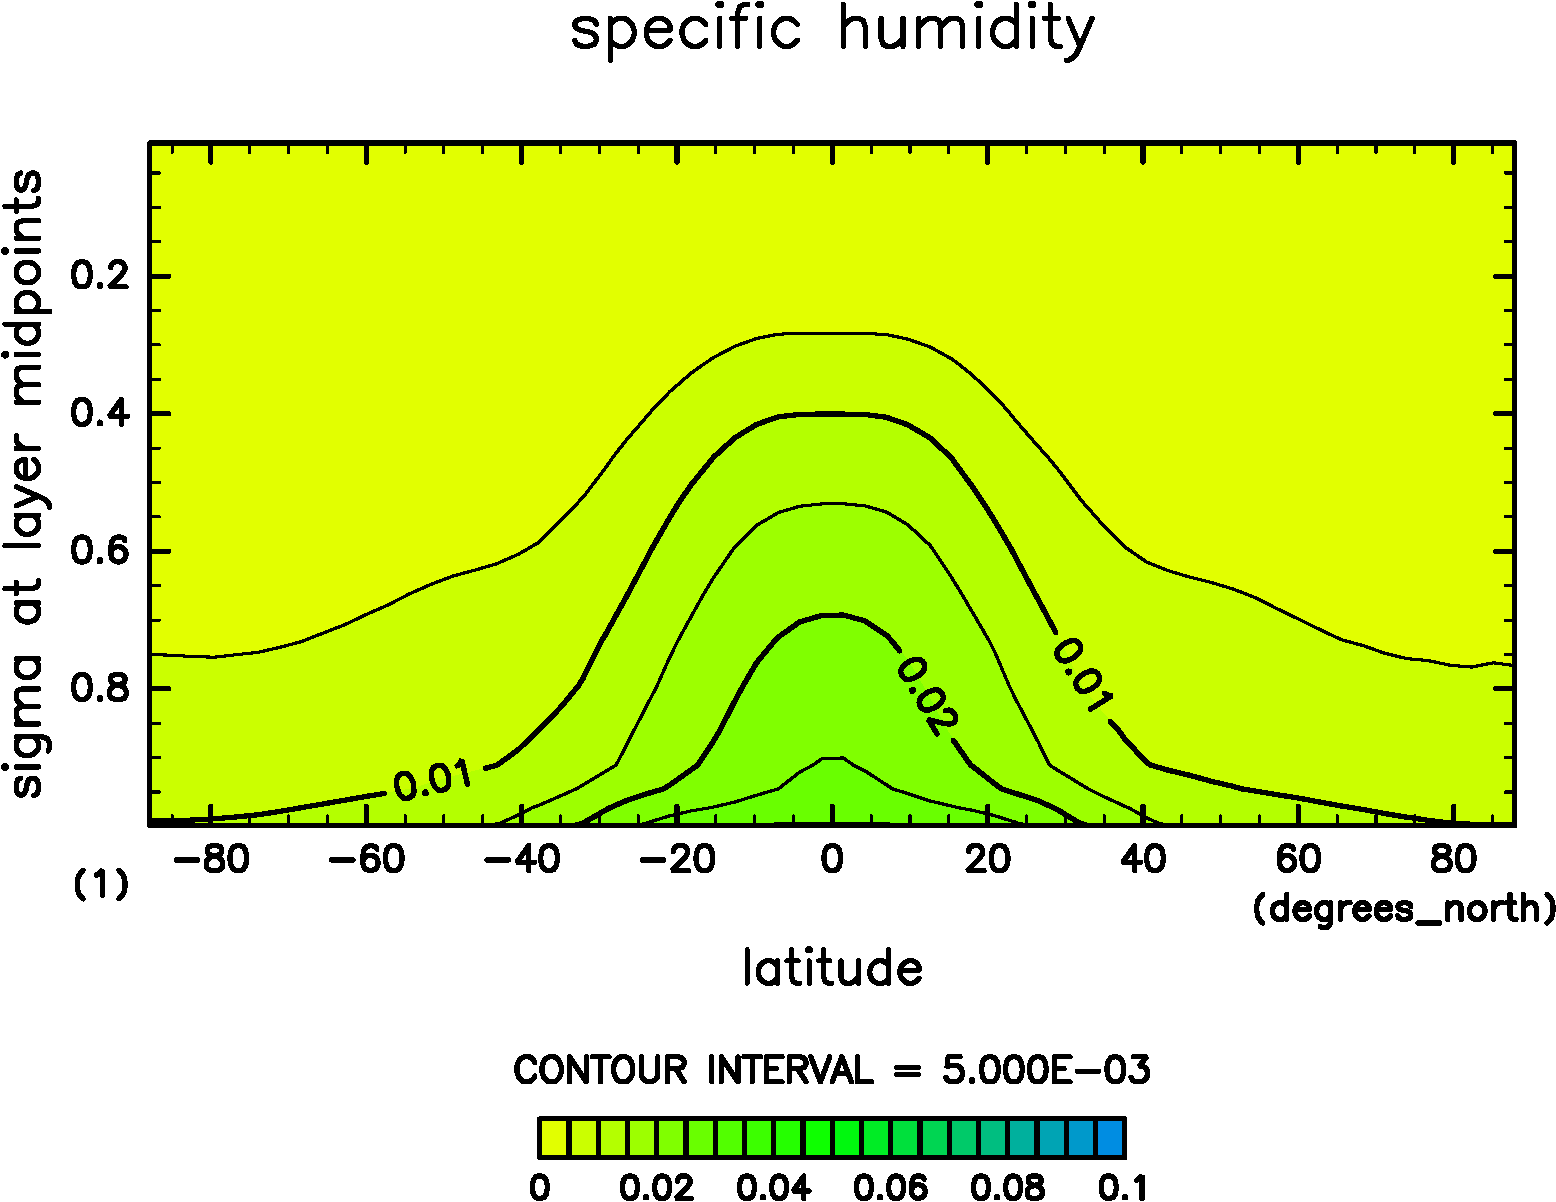
\includegraphics[width=\textwidth]{S1600/QH2OVap,time=3650:4015-crop-rotate.pdf}
		\caption{比湿\hmu*{[kg/kg]}}\label{S1600比湿}
	\end{subfigure}
	\begin{subfigure}{.4\textwidth}
		\centering
		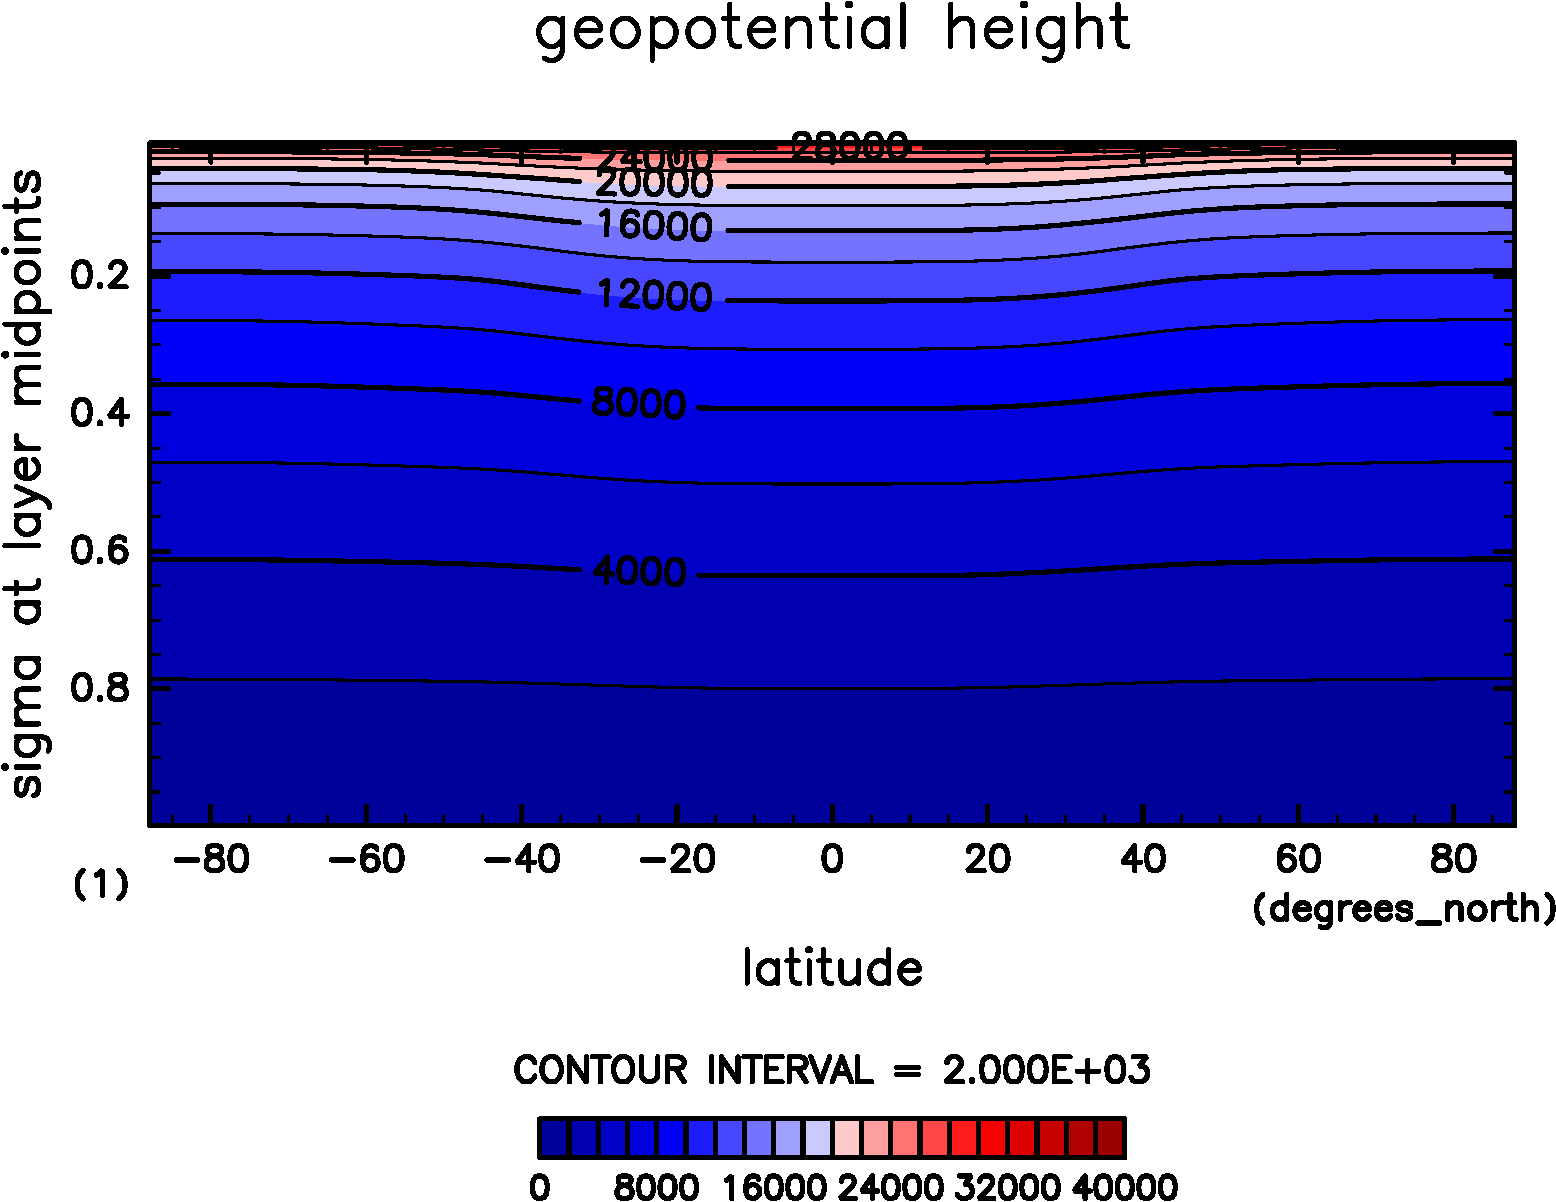
\includegraphics[width=\textwidth]{S1600/Height,time=3650:4015-crop-rotate.pdf}
		\caption{ジオポテンシャル高度\hmu*{[m]}}\label{S1600ジオポテンシャル高度}
	\end{subfigure}
	\caption[実験 S1600 の各物理量の子午面分布]{
		実験 S1600 の各物理量の子午面分布。図 \ref{S1366} と同様の図であるが、
		11 年目の年平均値である。
	}\label{S1600}
\end{figure}

\begin{figure}[t]
	\centering
	\begin{subfigure}{.4\textwidth}
		\centering
		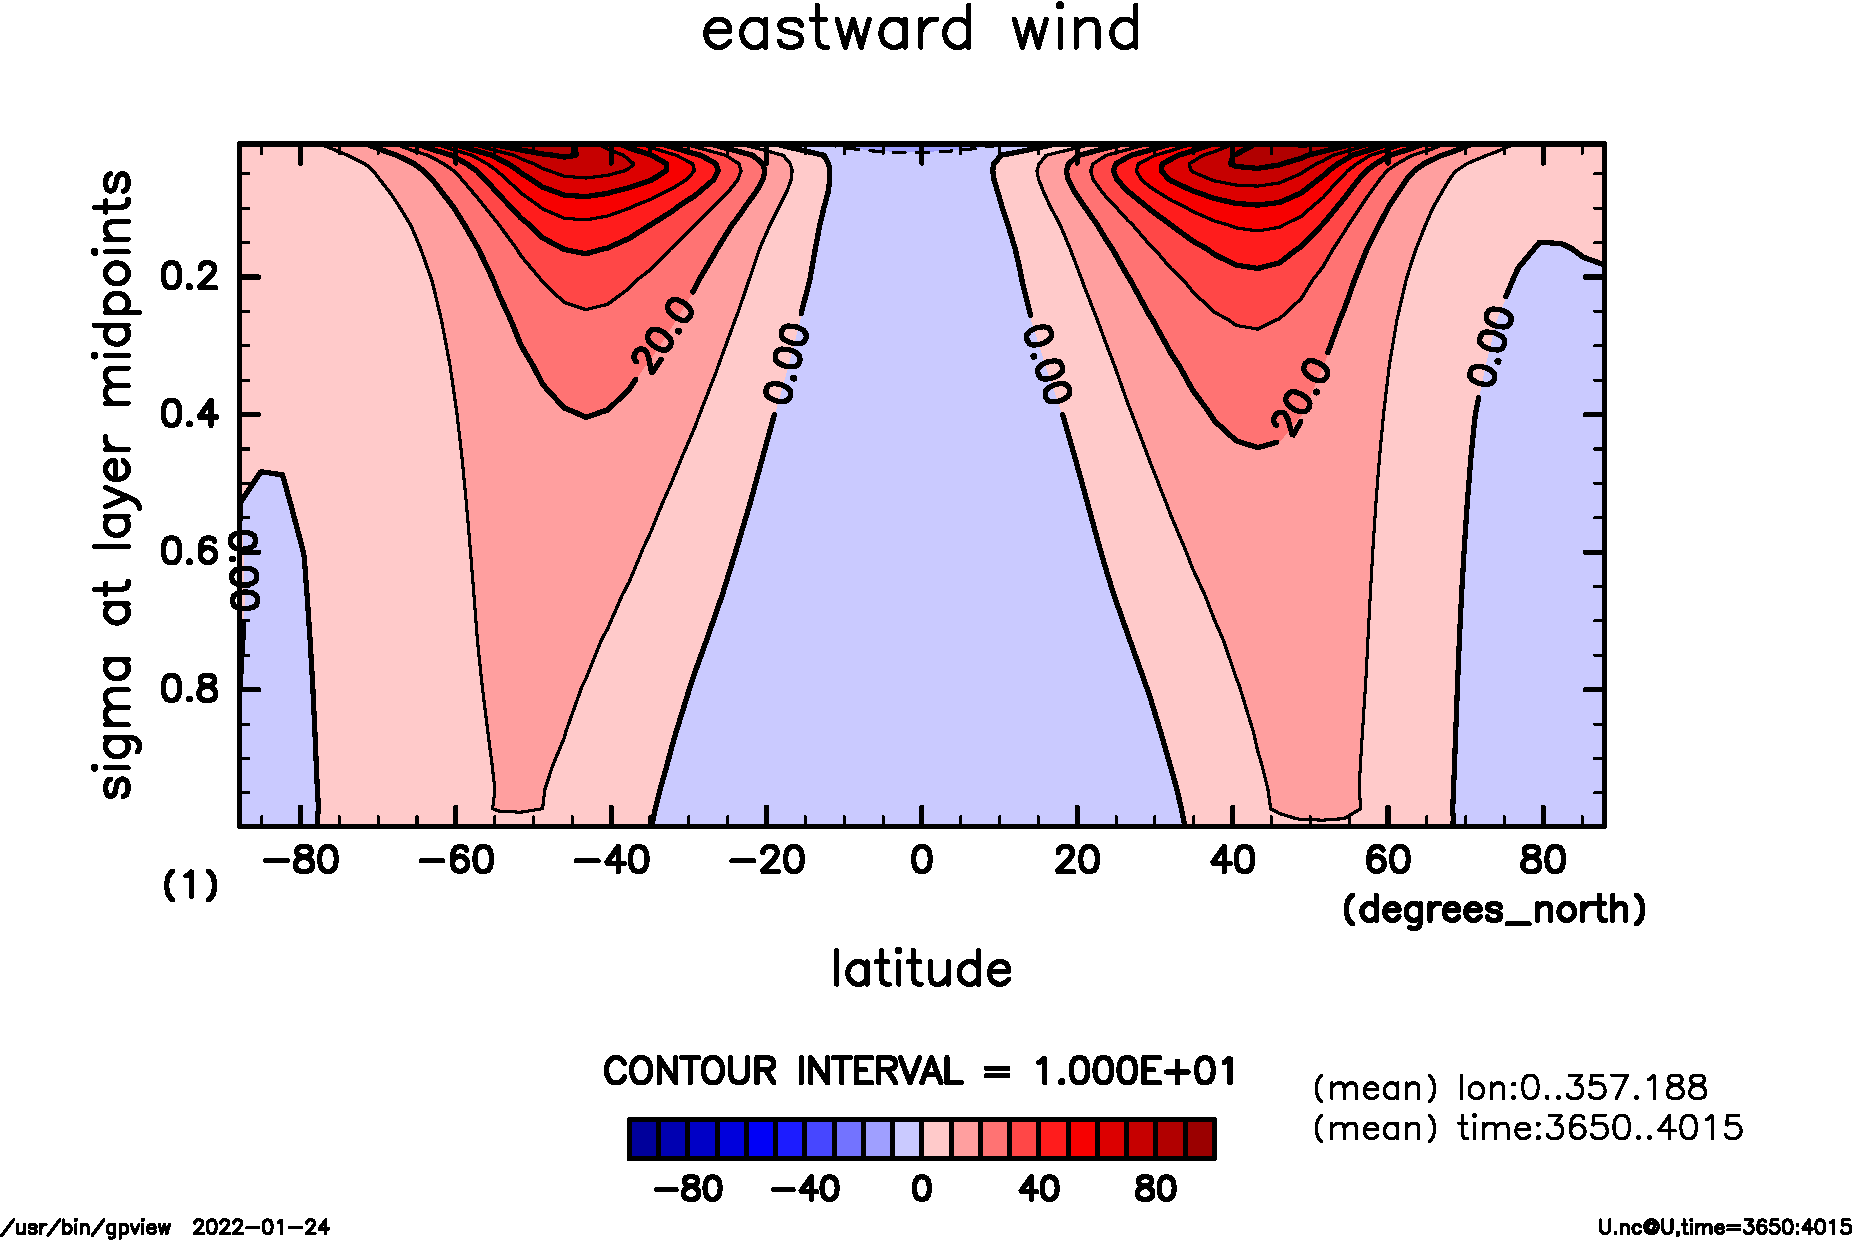
\includegraphics[width=\textwidth]{S1800/U,time=3650:4015-crop-rotate.pdf}
		\caption{東西風\hmu*{[m/s]}}\label{S1800東西風}
	\end{subfigure}
	\begin{subfigure}{.4\textwidth}
		\centering
		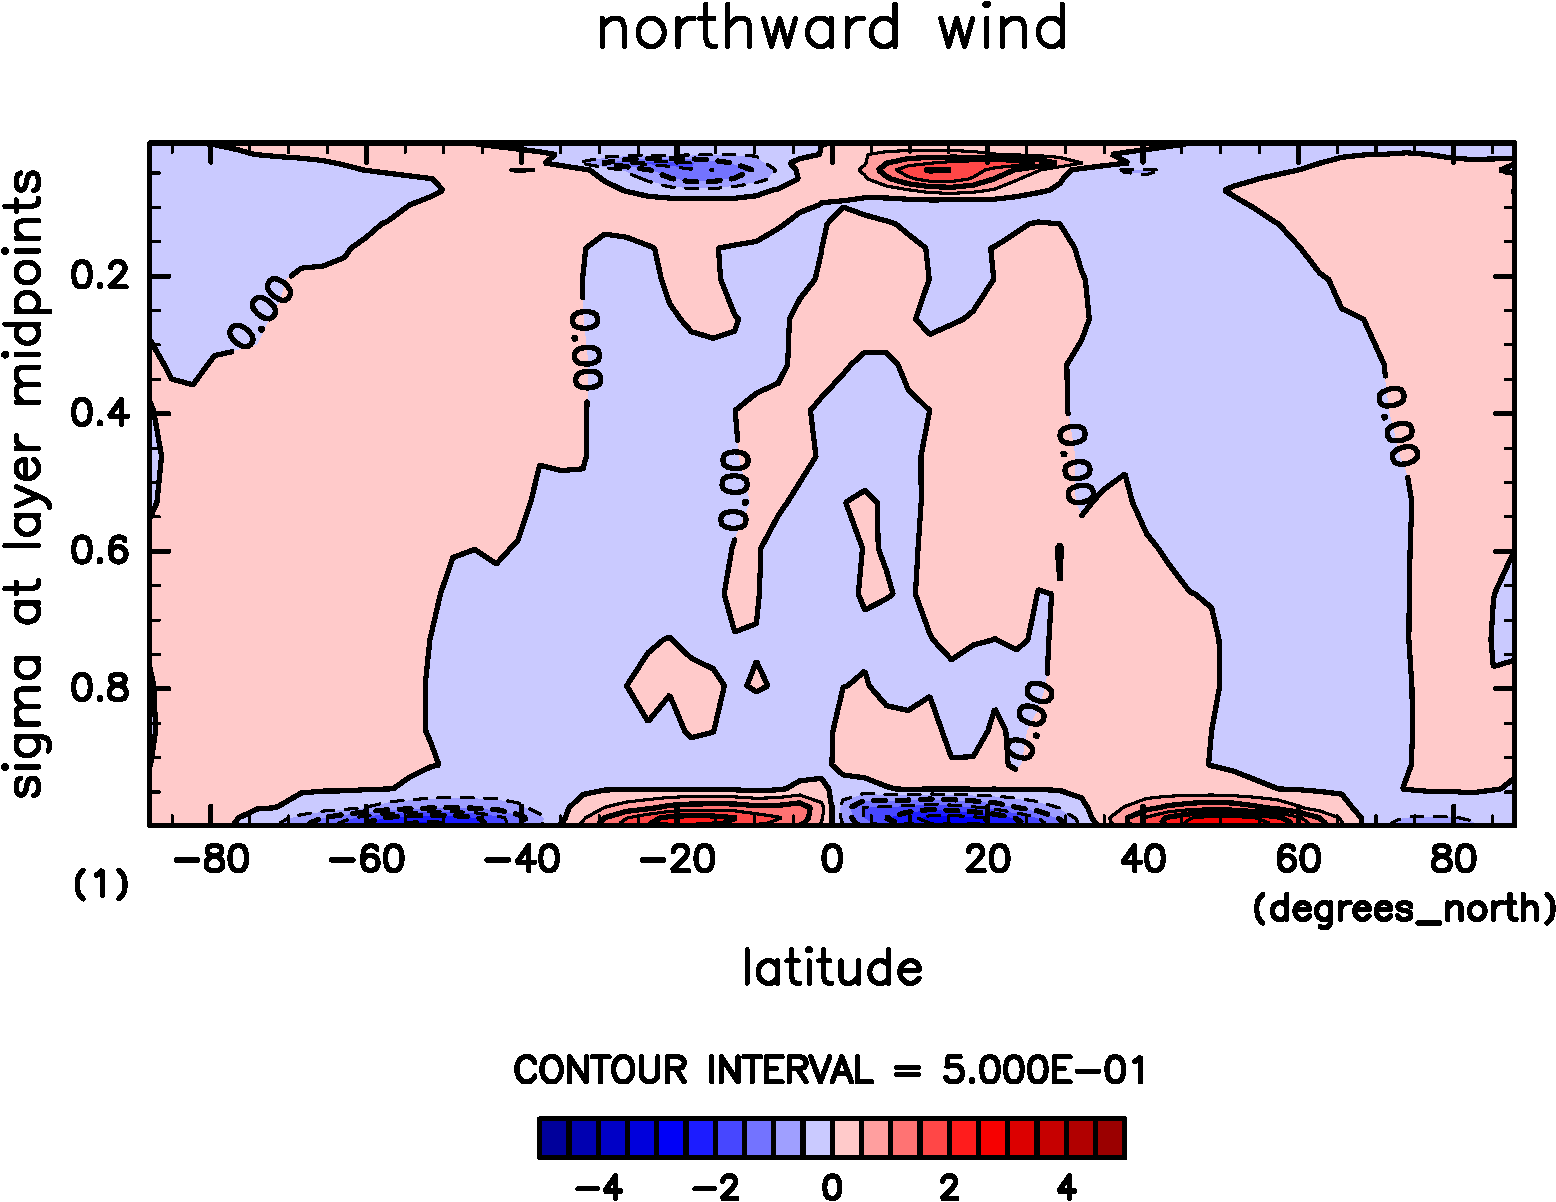
\includegraphics[width=\textwidth]{S1800/V,time=3650:4015-crop-rotate.pdf}
		\caption{南北風\hmu*{[m/s]}}\label{S1800南北風}
	\end{subfigure}
	\begin{subfigure}{.4\textwidth}
		\centering
		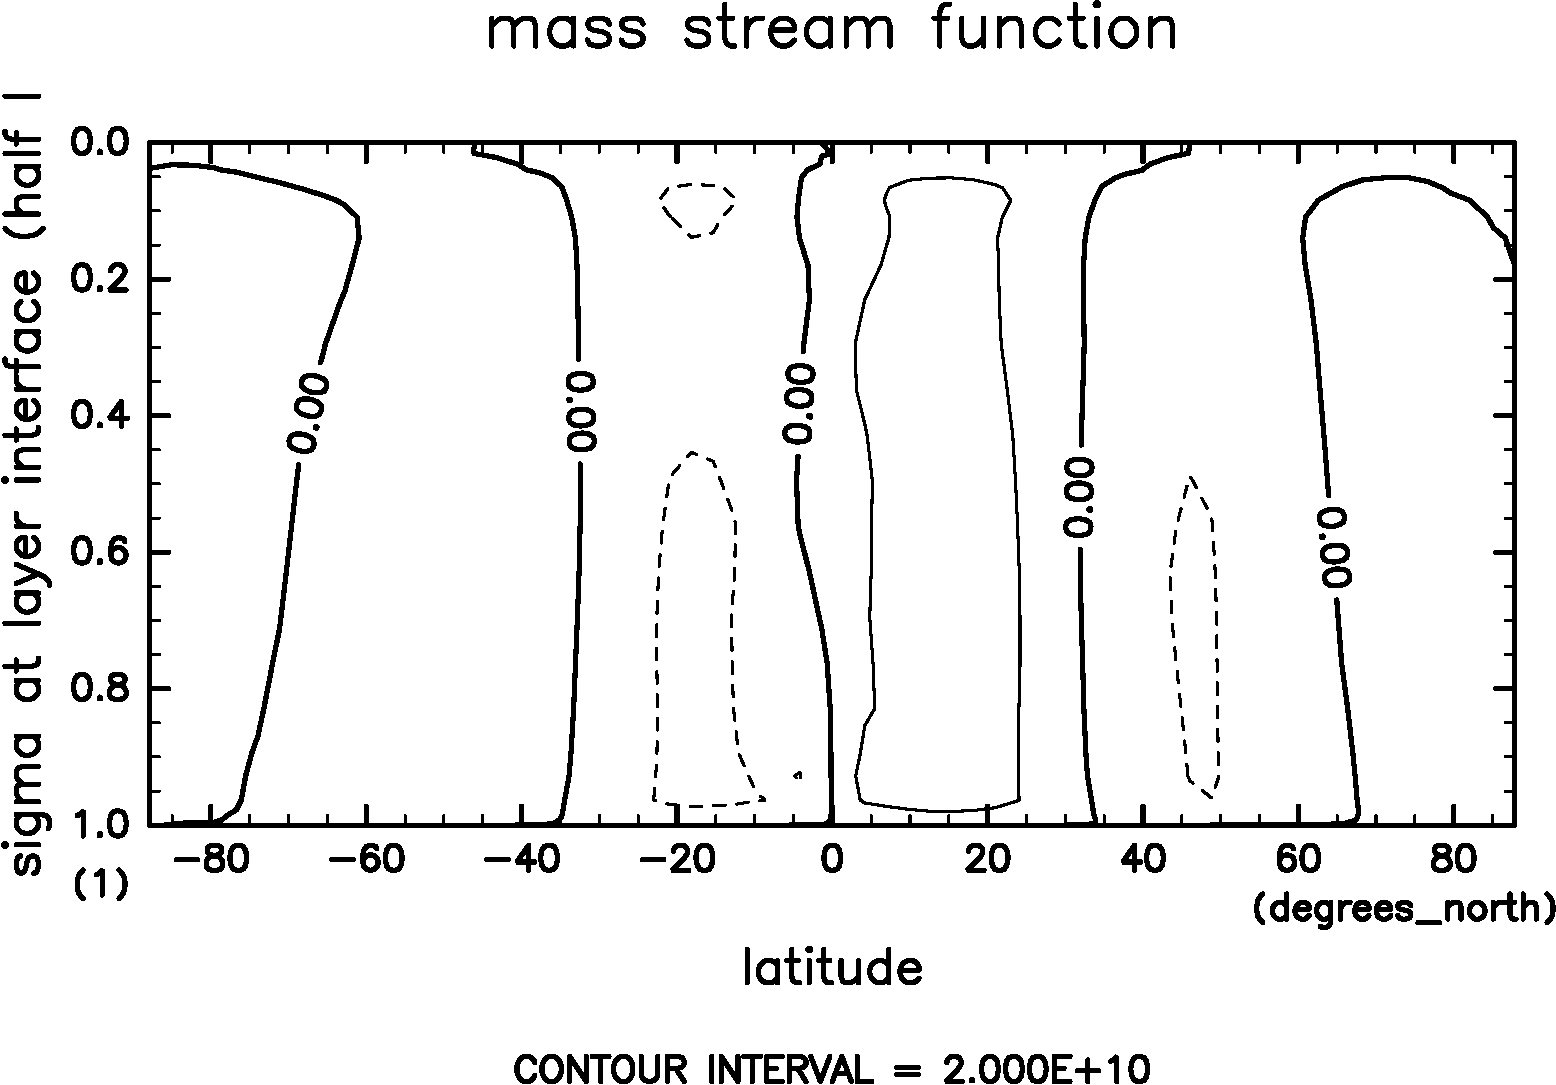
\includegraphics[width=\textwidth]{S1800/MSF,time=3650:4015-crop-rotate.pdf}
		\\\vspace{13pt}
		\caption{質量流線関数\hmu*{[kg/s]}}\label{S1800質量流線関数}
	\end{subfigure}
	\begin{subfigure}{.4\textwidth}
		\centering
		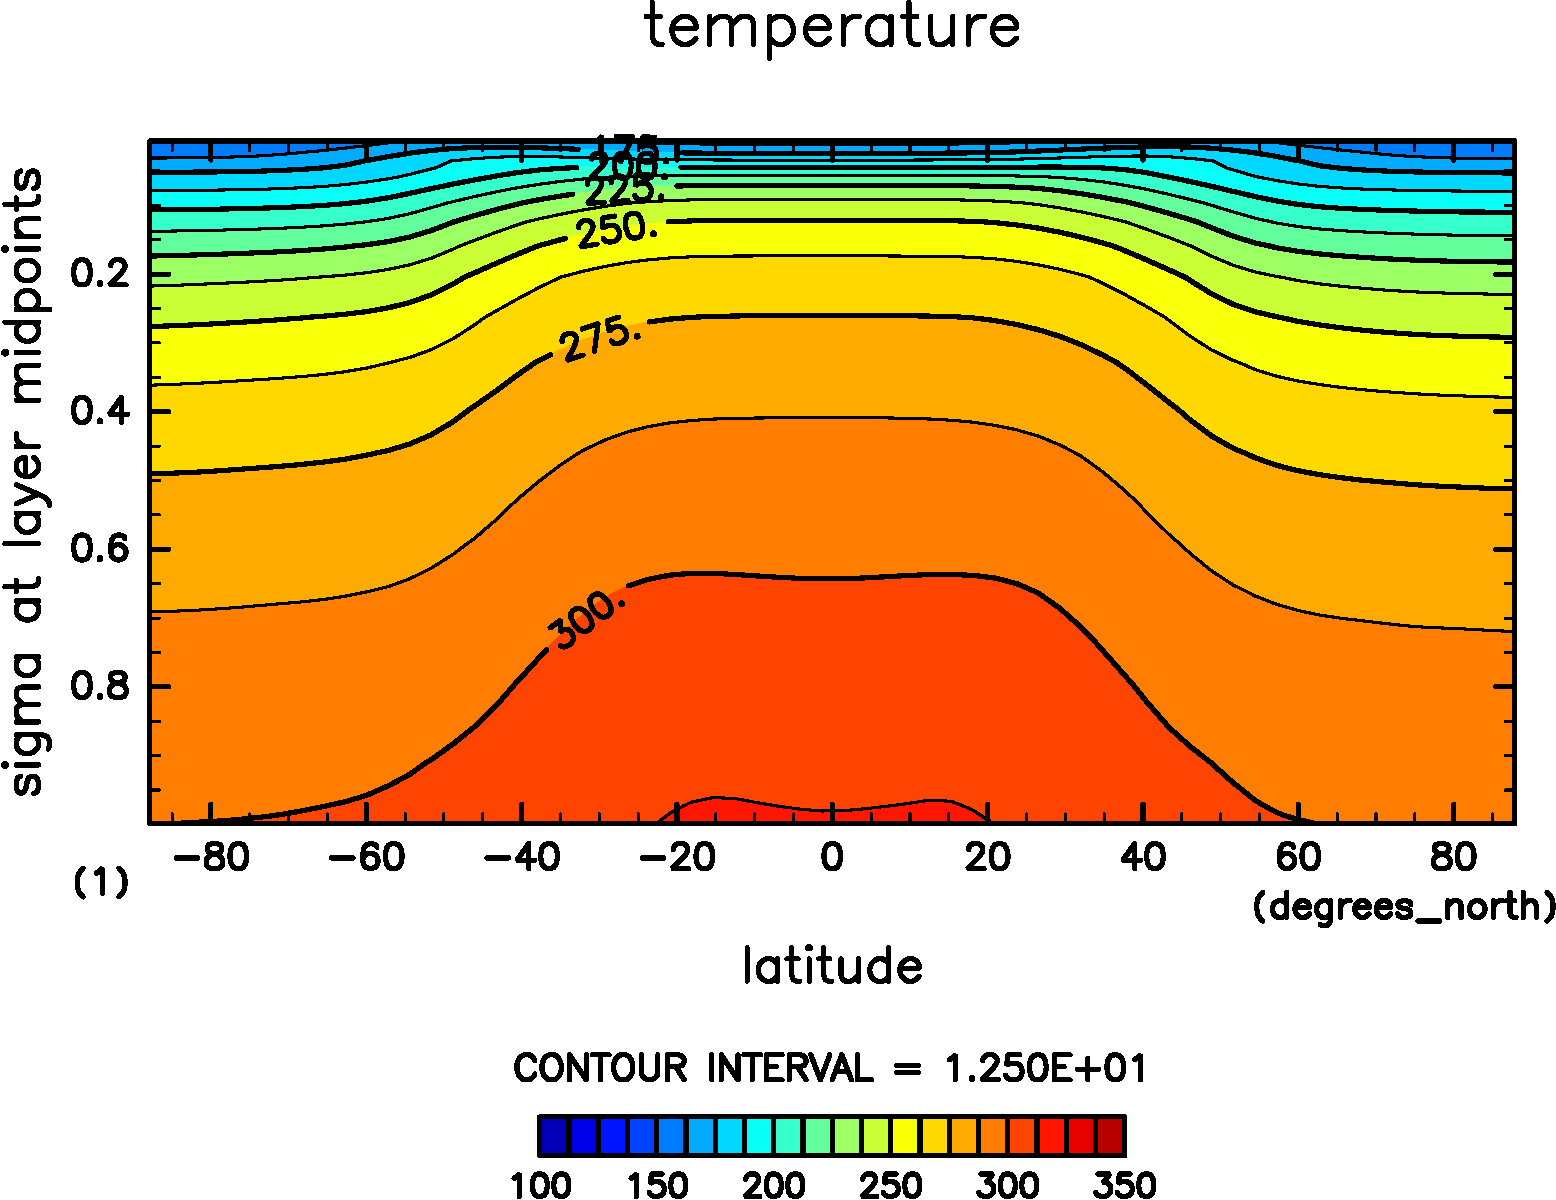
\includegraphics[width=\textwidth]{S1800/Temp,time=3650:4015-crop-rotate.pdf}
		\caption{気温\hmu*{[K]}}\label{S1800気温分布}
	\end{subfigure}
	\begin{subfigure}{.4\textwidth}
		\centering
		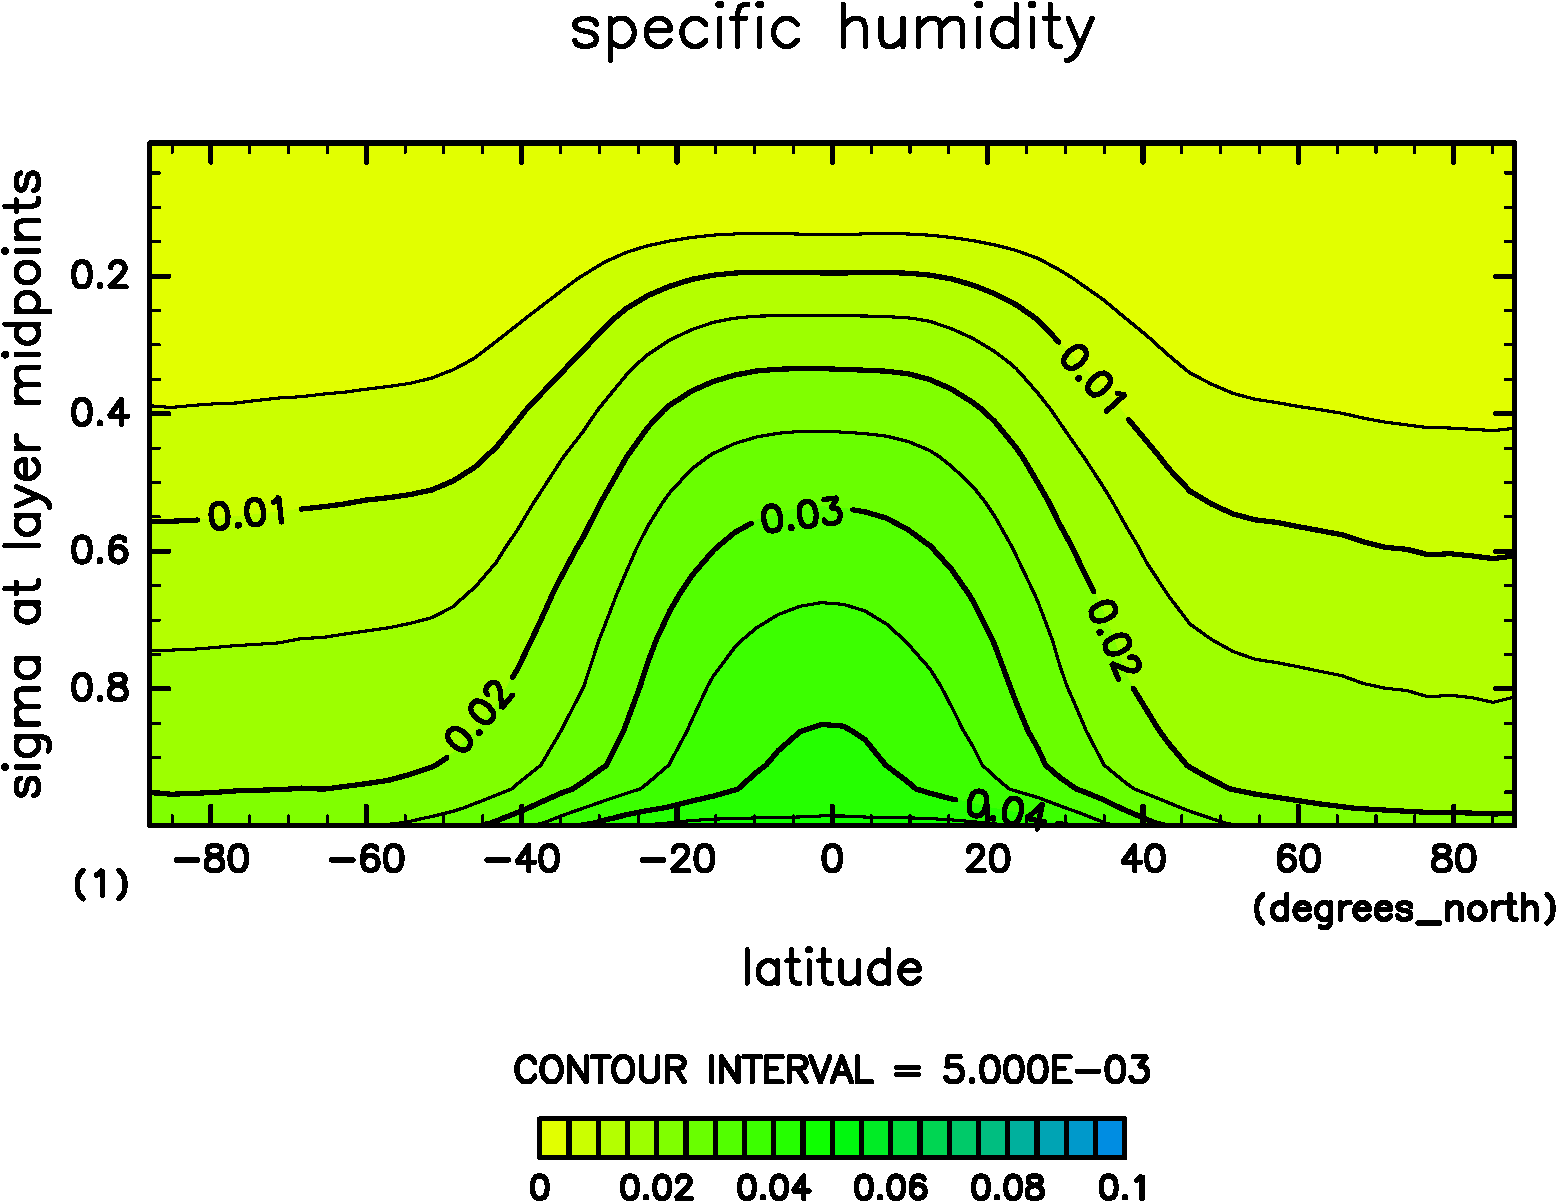
\includegraphics[width=\textwidth]{S1800/QH2OVap,time=3650:4015-crop-rotate.pdf}
		\caption{比湿\hmu*{[kg/kg]}}\label{S1800比湿}
	\end{subfigure}
	\begin{subfigure}{.4\textwidth}
		\centering
		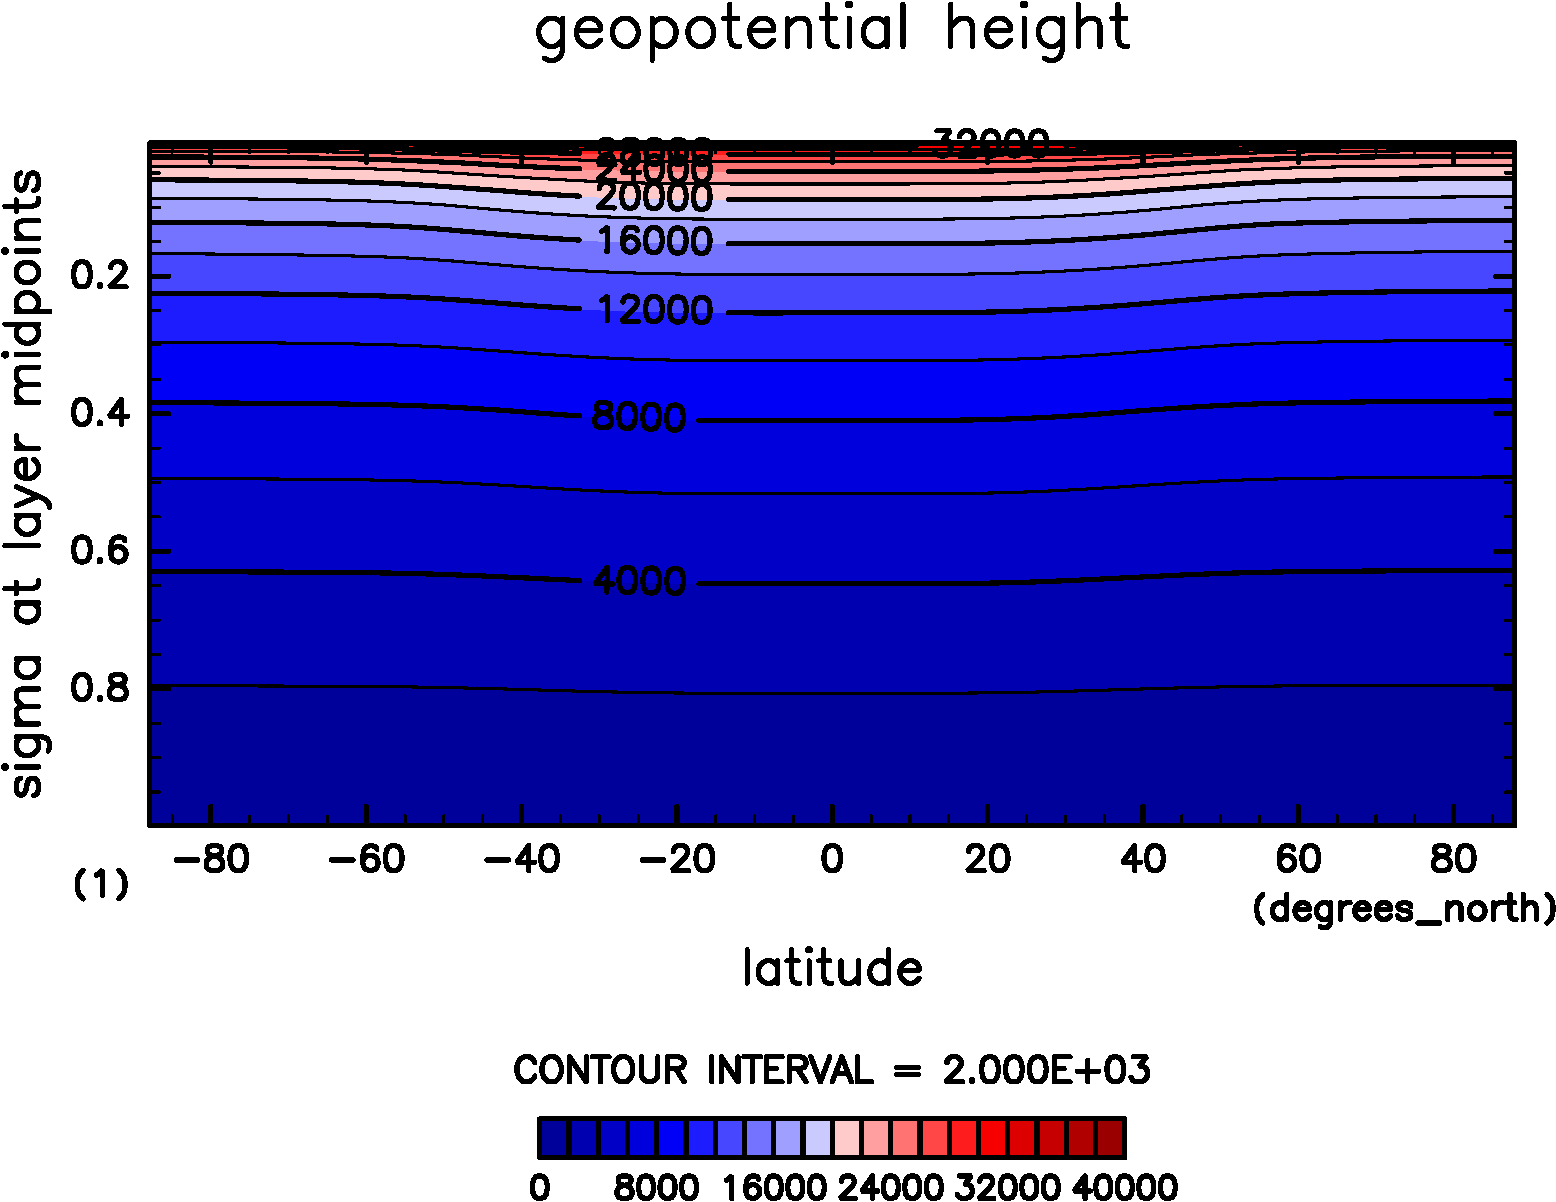
\includegraphics[width=\textwidth]{S1800/Height,time=3650:4015-crop-rotate.pdf}
		\caption{ジオポテンシャル高度\hmu*{[m]}}\label{S1800ジオポテンシャル高度}
	\end{subfigure}
	\caption[実験 S1800 の各物理量の子午面分布]{
		実験 S1800 の各物理量の子午面分布。図 \ref{S1366} と同様の図であるが、
		11 年目の年平均値である。
	}\label{S1800}
\end{figure}

\begin{figure}[t]
	\centering
	\begin{subfigure}{.4\textwidth}
		\centering
		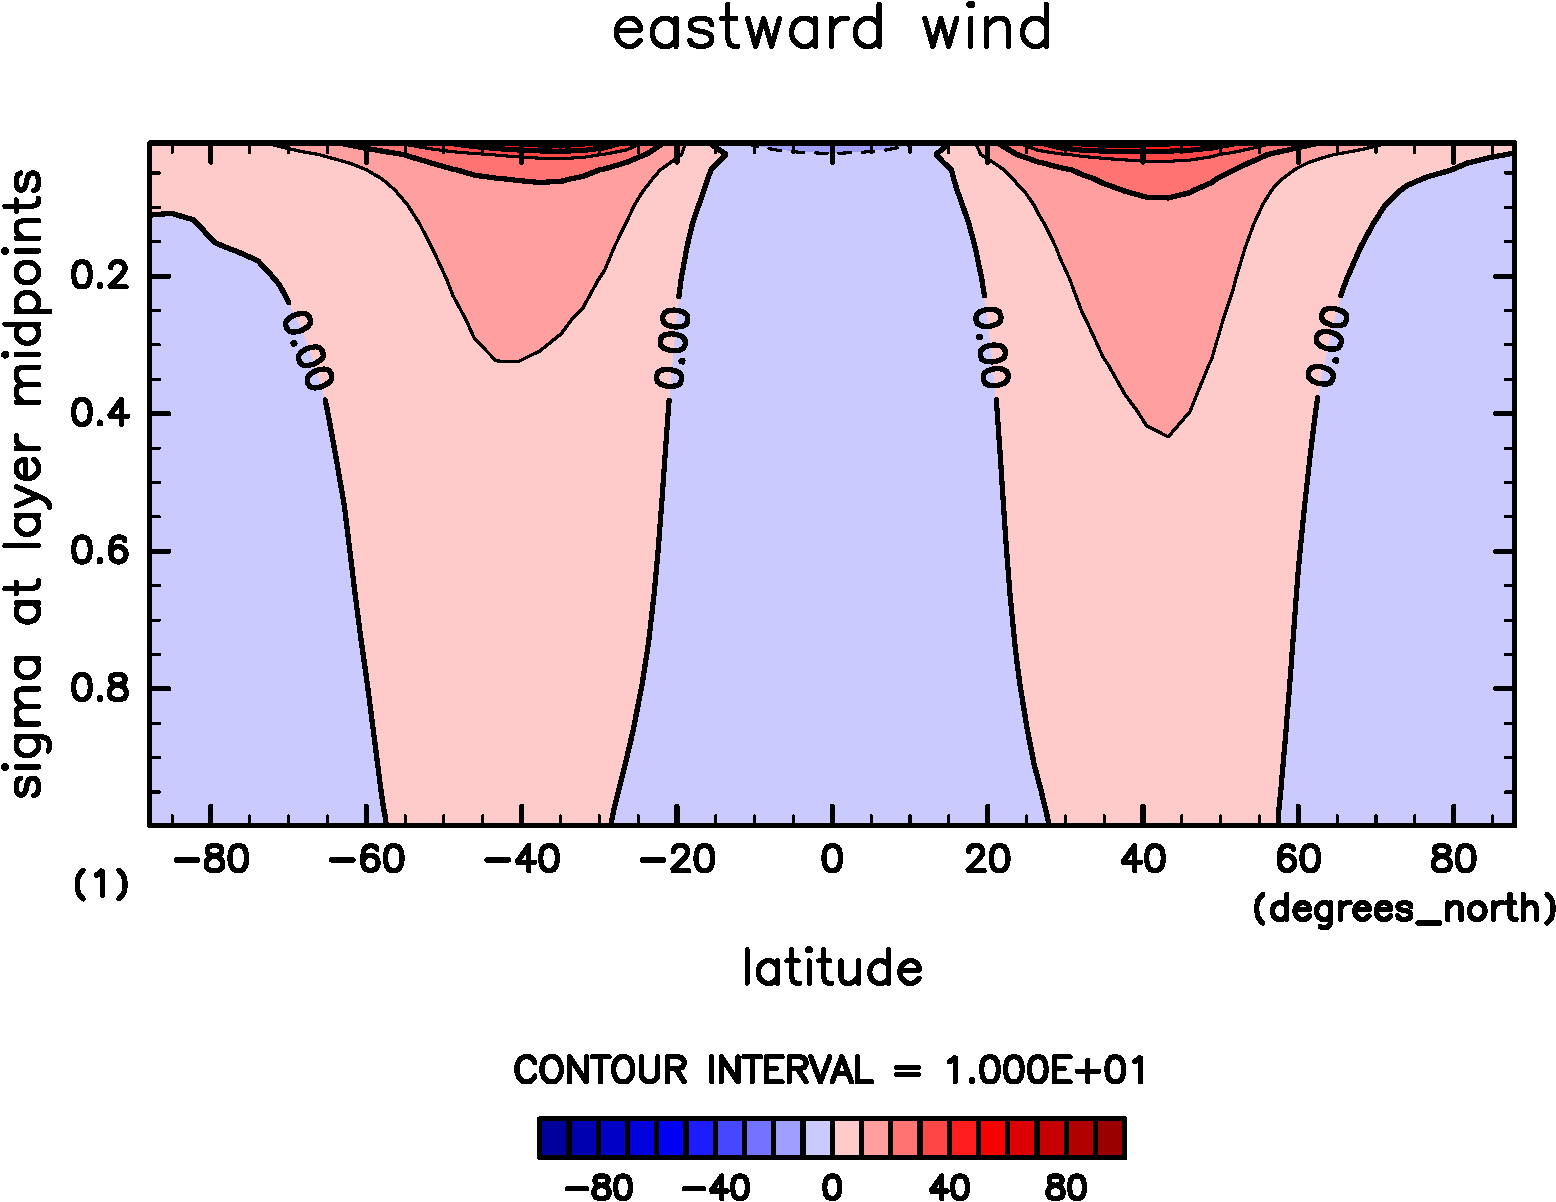
\includegraphics[width=\textwidth]{S2000/U,time=7300:7665-crop-rotate.pdf}
		\caption{東西風\hmu*{[m/s]}}\label{S2000東西風}
	\end{subfigure}
	\begin{subfigure}{.4\textwidth}
		\centering
		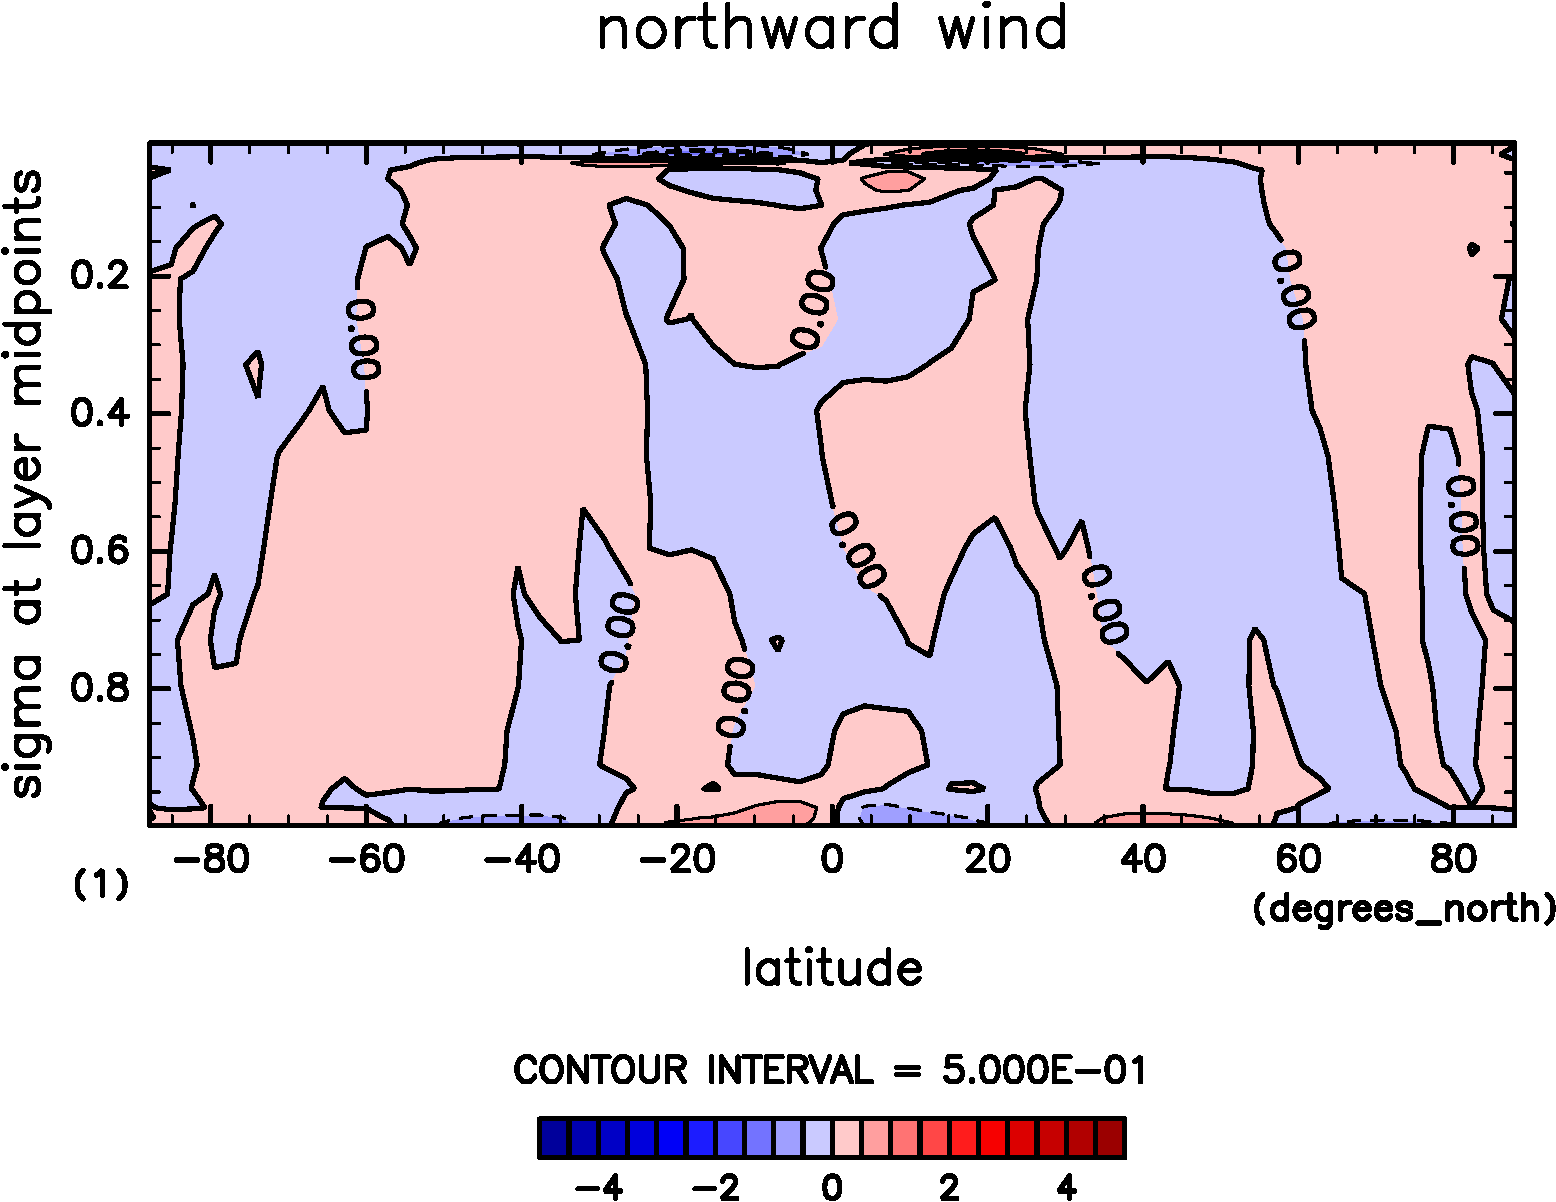
\includegraphics[width=\textwidth]{S2000/V,time=7300:7665-crop-rotate.pdf}
		\caption{南北風\hmu*{[m/s]}}\label{S2000南北風}
	\end{subfigure}
	\begin{subfigure}{.4\textwidth}
		\centering
		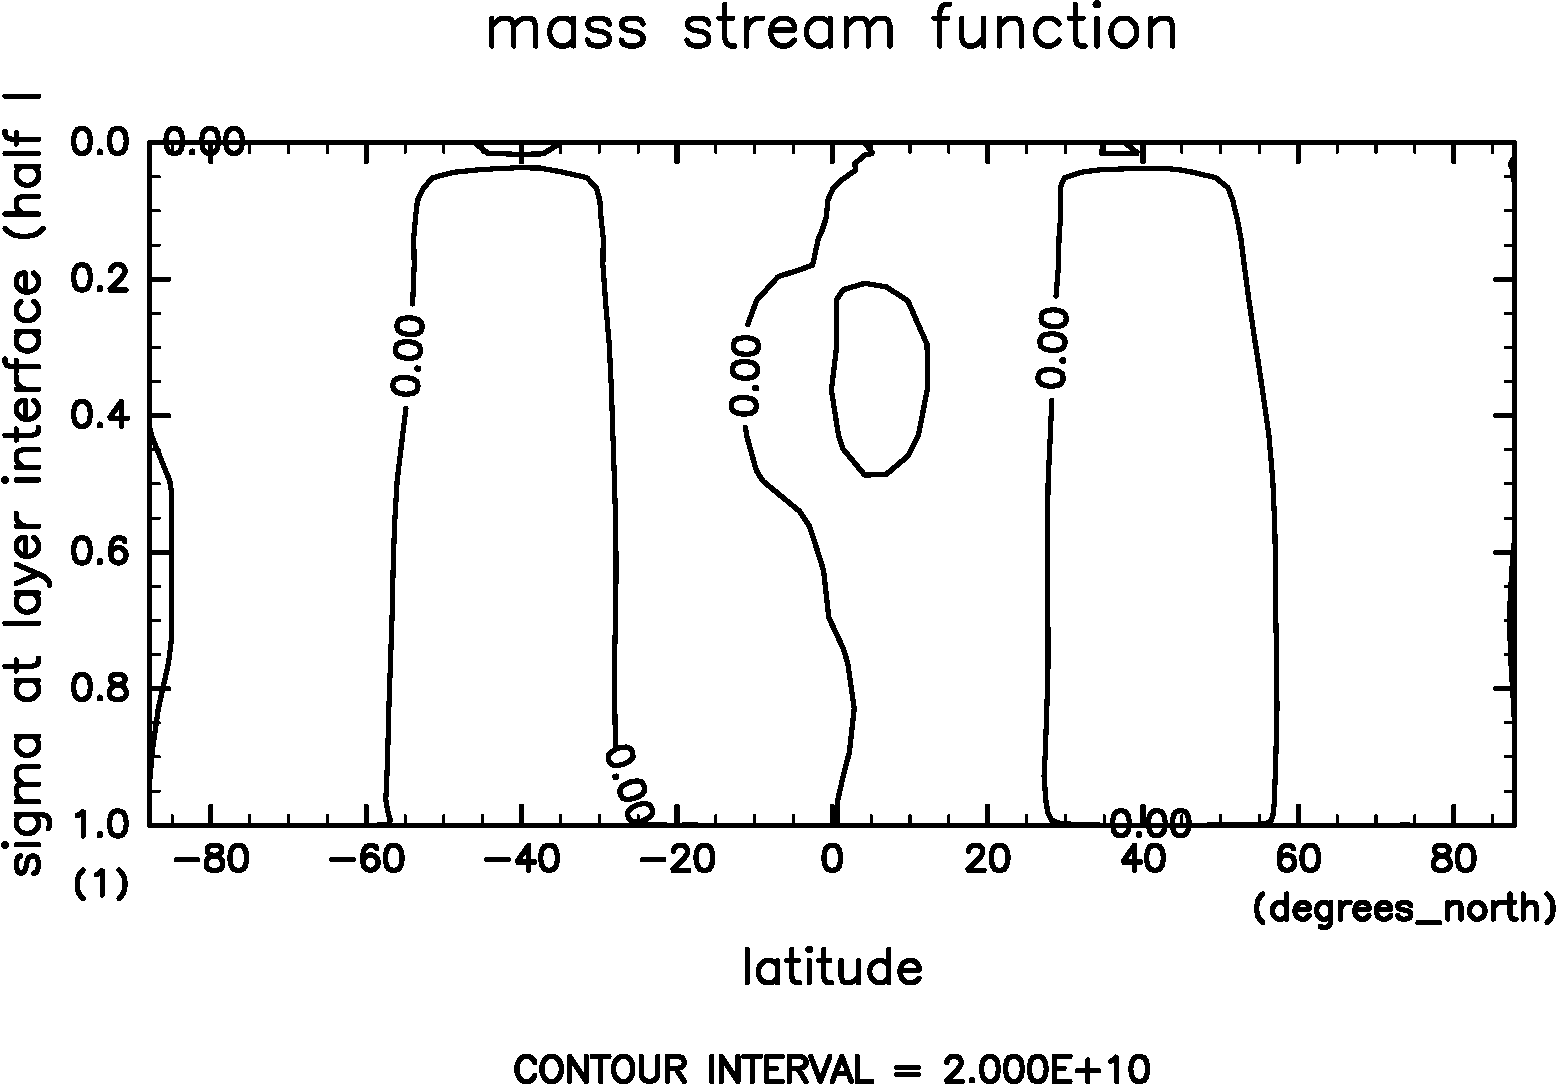
\includegraphics[width=\textwidth]{S2000/MSF,time=7300:7665-crop-rotate.pdf}
		\\\vspace{13pt}
		\caption{質量流線関数\hmu*{[kg/s]}}\label{S2000質量流線関数}
	\end{subfigure}
	\begin{subfigure}{.4\textwidth}
		\centering
		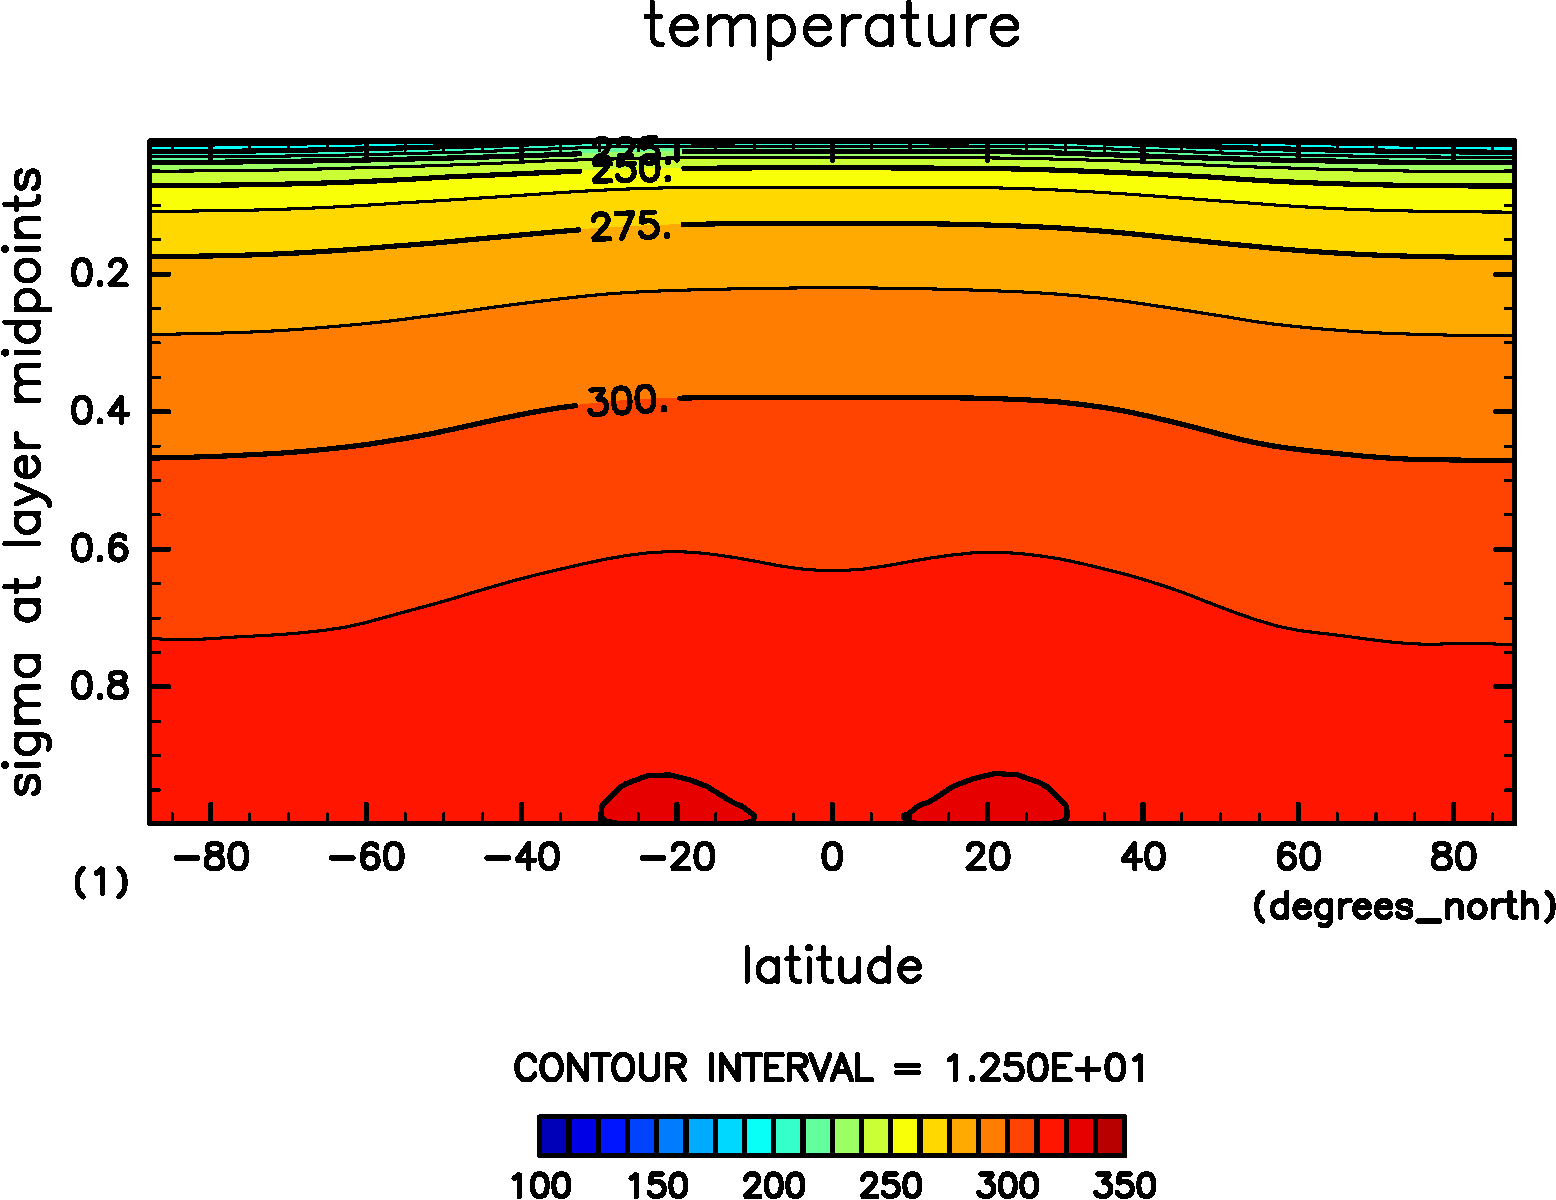
\includegraphics[width=\textwidth]{S2000/Temp,time=7300:7665-crop-rotate.pdf}
		\caption{気温\hmu*{[K]}}\label{S2000気温分布}
	\end{subfigure}
	\begin{subfigure}{.4\textwidth}
		\centering
		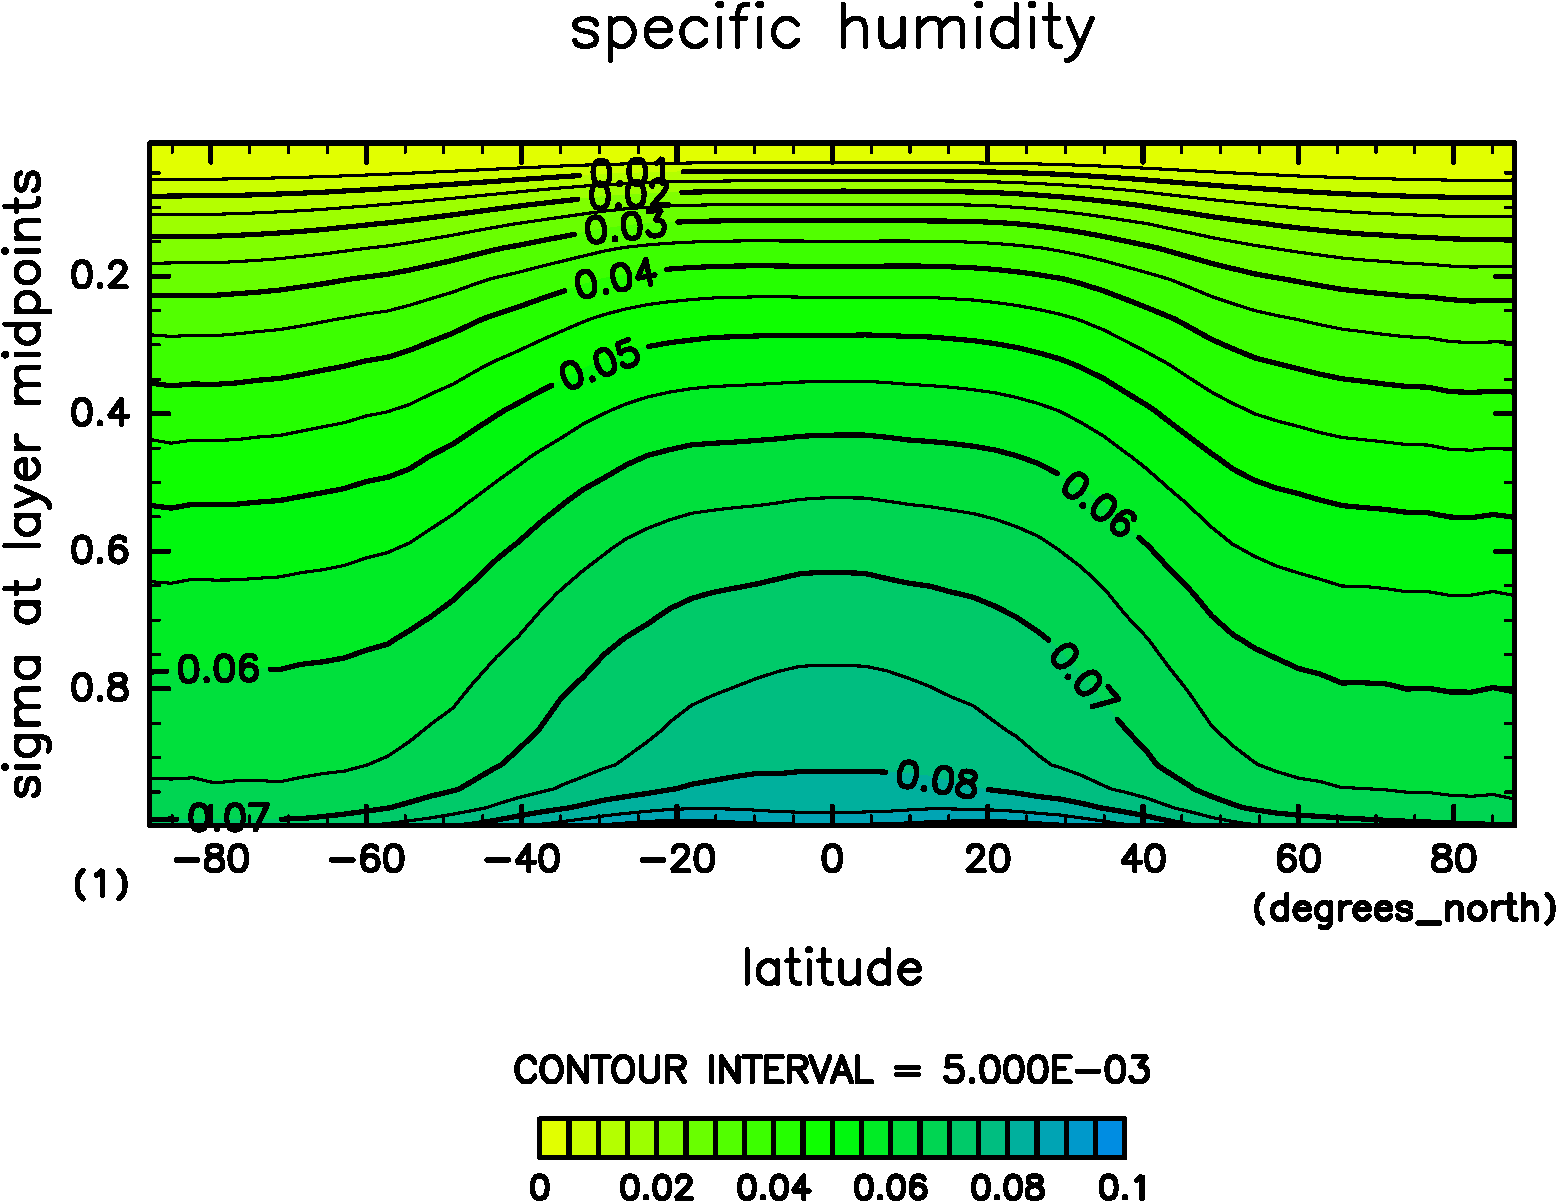
\includegraphics[width=\textwidth]{S2000/QH2OVap,time=7300:7665-crop-rotate.pdf}
		\caption{比湿\hmu*{[kg/kg]}}\label{S2000比湿}
	\end{subfigure}
	\begin{subfigure}{.4\textwidth}
		\centering
		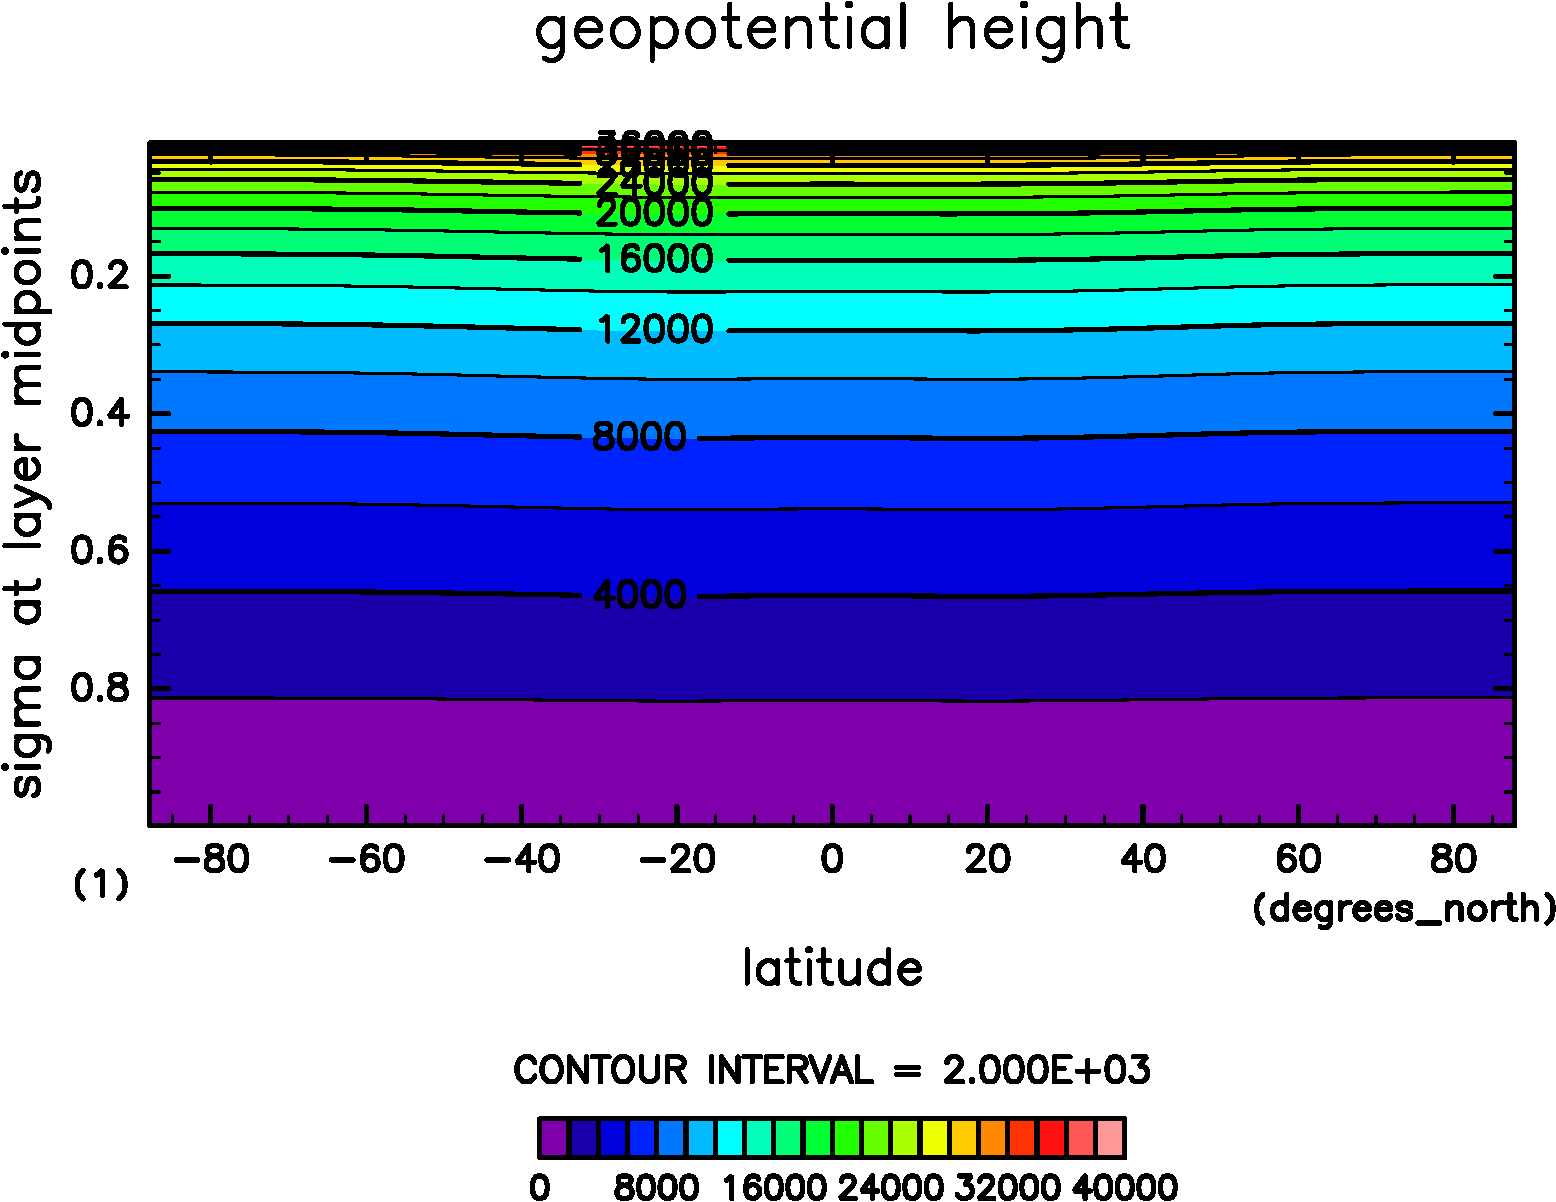
\includegraphics[width=\textwidth]{S2000/Height,time=7300:7665-crop-rotate.pdf}
		\caption{ジオポテンシャル高度\hmu*{[m]}}\label{S2000ジオポテンシャル高度}
	\end{subfigure}
	\caption[実験 S2000 の各物理量の子午面分布]{
		実験 S2000 の各物理量の子午面分布。図 \ref{S1366} と同様の図であるが、
		21 年目の年平均値である。
	}\label{S2000}
\end{figure}

\afterpage{\clearpage}

\section{雲がある場合の南北熱輸送の太陽定数依存性}

ここまで、雲あり各実験でどのような子午面構造が現れているかをみてきた。
次からは、雲あり各実験で、どのような南北熱輸送が起きているかを示す。
南北熱輸送を \(F_T=F_D+F_L\) と書く。
ここで、\(F_L\) は潜熱による南北熱輸送で、
\(F_D\) は乾燥静的エネルギーによる熱輸送である。
乾燥静的エネルギーはエンタルピーとジオポテンシャルの和であるから、
それぞれ式で表せば以下のようになる。
\begin{gather}
	F_T=F_L+F_D,\\
	\begin{split}
		F_L&=\overline{\qty[\int^{z_\text{top}}_0 \rho Lqv\,dz]}\\
		&=\overline{\qty[\int^{p_s}_0 \rho Lqv\frac{dp}{g}]}\\
		&=\overline{\qty[\int^1_0 \qty(\frac{Lqv}{g}p_s)\,d\sigma]}\\
		&=\int^1_0 \qty[\overline{Lqv\frac{p_s}{g}}]d\sigma,
	\end{split}\\
	\begin{split}
		F_D&=\overline{\qty[\int^{z_\text{top}}_0 \rho (c_{pn}T+gz)v\,dz]}\\
		&=\overline{\qty[\int^{p_s}_0 \rho (c_{pn}T+gz)v\frac{dp}{g}]}\\
		&=\overline{\qty[\int^1_0 \qty(\frac{(c_{pn}T+gz)v}{g}p_s)\,d\sigma]}\\
		&=\int^1_0 \qty[\overline{(c_{pn}T+gz)v\frac{p_s}{g}}]d\sigma,
	\end{split}
\end{gather}
ここで、\([\bullet]\) は東西平均、\(\bar\bullet\) は時間平均、\(z_\text{top}\) は大気上端である。

\afterpage{\clearpage}

図 \ref{EnFlx} に雲あり各実験での南北熱輸送量を示した。
まず最初に全熱輸送量(各図の青線)に関して見る。全熱輸送量は赤道に関して対称で、
中緯度にピークがある事がわかる。
北半球の全熱輸送を見ると、
実験 S1366(図 \ref{EnFlxS1366})では北緯 30\textdegree に \(4.0\hmu{PW}\)、
実験 S1500(図 \ref{EnFlxS1500})では北緯 30\textdegree に \(4.2\hmu{PW}\)、
実験 S1600(図 \ref{EnFlxS1600})では北緯 30\textdegree に \(4.5\hmu{PW}\)、
実験 S1800(図 \ref{EnFlxS1800})では北緯 35\textdegree に \(5.0\hmu{PW}\)、
実験 S2000(図 \ref{EnFlxS2000})では北緯 40\textdegree に \(3.0\hmu{PW}\)
の高緯度向きの輸送量のピークがある。
このように、実験 S1366 から実験 S1800 までは、太陽定数が増大するにつれて、
全熱輸送量のピークの値も増大している。しかし、実験 S2000 では全熱輸送量が減少している。
%全熱輸送量は、実験 S1366(図 \ref{EnFlxS1366}) から実験 S1800
%(図 \ref{EnFlxS1800})までは太陽定数が大きくなるにつれて増大して
%いる。実験 S2000 では小さくなっている。
%これは、実験 S2000 では南北風が小さくなっており(図 \ref{S2000南北風})、
%熱の輸送量が小さくなっているからである。

熱輸送量の合計を見たので、次は潜熱輸送と乾燥静的エネルギー輸送に分けて見る。
潜熱輸送は、低緯度で低緯度向きの、中緯度で高緯度向きのピークがある(図 \ref{EnFlx})
が、実験 S2000 はパターンが違うようにみえる。
低緯度での低緯度向きの輸送量のピークの値は、
実験 S1366(図 \ref{EnFlxS1366})では北緯 10\textdegree で \(3.0\hmu{PW}\)、
実験 S1500(図 \ref{EnFlxS1500})では北緯 10\textdegree で \(3.0\hmu{PW}\)、
実験 S1600(図 \ref{EnFlxS1600})では北緯 10\textdegree で \(2.5\hmu{PW}\)、
実験 S1800(図 \ref{EnFlxS1800})では北緯 10\textdegree で \(1.5\hmu{PW}\)、
実験 S2000(図 \ref{EnFlxS2000})では北緯 20\textdegree で \(0.5\hmu{PW}\)
となっといて、太陽定数が増大するに従って高緯度側に移動し減少している。
実験 S1800 までは同じパターンを有しており、太陽定数が増大するにつれて、
潜熱輸送のピークの緯度が高緯度に移動する。
中緯度での高緯度向きの輸送量のピークの値は、
実験 S1366(図 \ref{EnFlxS1366})では北緯 30\textdegree で \(3.5\hmu{PW}\)、
実験 S1500(図 \ref{EnFlxS1500})では北緯 35\textdegree で \(4.5\hmu{PW}\)、
実験 S1600(図 \ref{EnFlxS1600})では北緯 35\textdegree で \(4.5\hmu{PW}\)、
実験 S1800(図 \ref{EnFlxS1800})では北緯 40\textdegree で \(5.5\hmu{PW}\)、
実験 S2000(図 \ref{EnFlxS2000})では北緯 40\textdegree で \(4.0\hmu{PW}\)
となっていて、実験 S1366 から 実験 S1800 では太陽定数が増大するに従って、
高緯度側に移動し輸送量は増大する。一方で実験 S2000 では輸送量は減少している。
%実験 S1800 まで太陽定数が
%大きくなるに従って潜熱輸送が大きくなるのは、太陽定数が大きくなるにつれて
%比湿の値が大きくなっている(図 \ref{S1366比湿} から \ref{S2000比湿})からだと考えられる。
%実験 S2000 で潜熱輸送が小さくなるのは、南北風が小さくなる(図 \ref{S2000南北風})からである。
%潜熱輸送は低緯度と中緯度に極値を持っている。これは、それぞれハドレー循環に
%よる地表付近での低緯度向きの輸送と、フェレル循環による地表付近での高緯度向き
%の輸送に対応している。比湿の値は太陽定数の増大に伴って大きくなるので、潜熱
%輸送も太陽定数の増大に伴って大きくなる。

乾燥静的エネルギー輸送は、低緯度で高緯度向きの、中緯度で低緯度向きの
ピークがある(図 \ref{EnFlx})
が、実験 S2000 はパターンが違うようにみえる。
低緯度での輸送量のピークの値は、
実験 S1366(図 \ref{EnFlxS1366})では北緯 10\textdegree で \(3.0\hmu{PW}\)、
実験 S1500(図 \ref{EnFlxS1500})では北緯 10\textdegree で \(3.0\hmu{PW}\)、
実験 S1600(図 \ref{EnFlxS1600})では北緯 10\textdegree で \(2.5\hmu{PW}\)、
実験 S1800(図 \ref{EnFlxS1800})では北緯 10\textdegree で \(1.5\hmu{PW}\)、
実験 S2000(図 \ref{EnFlxS2000})では北緯 20\textdegree で \(0.5\hmu{PW}\)
となっといて、太陽定数が増大するに従って高緯度側に移動し減少している。
実験 S1800 までは同じパターンを有しており、太陽定数が増大するにつれて、
潜熱輸送のピークの緯度が高緯度に移動する。
中緯度での輸送量のピークの値は、
実験 S1366(図 \ref{EnFlxS1366})では北緯 30\textdegree で \(3.5\hmu{PW}\)、
実験 S1500(図 \ref{EnFlxS1500})では北緯 35\textdegree で \(4.5\hmu{PW}\)、
実験 S1600(図 \ref{EnFlxS1600})では北緯 35\textdegree で \(4.5\hmu{PW}\)、
実験 S1800(図 \ref{EnFlxS1800})では北緯 40\textdegree で \(5.5\hmu{PW}\)、
実験 S2000(図 \ref{EnFlxS2000})では北緯 40\textdegree で \(4.0\hmu{PW}\)
となっていて、実験 S1366 から 実験 S1800 では太陽定数が増大するに従って、
高緯度側に移動し輸送量は増大する。一方で実験 S2000 では輸送量は減少している。
%乾燥静的エネルギーの南北輸送は実験 S1500 で最大になり、それより
%太陽定数を大きくすると乾燥静的エネルギーの南北輸送は減少してゆく。
%これは、太陽定数が大きくなるにつれて、南北風が小さくなっていることが
%原因だと考えられる(図 \ref{S1366南北風} から図 \ref{S2000南北風})。
%実験 S1366 よりも実験 S1500 の方が乾燥静的エネルギーの輸送が
%大きいのは、実験 S1366 と実験 S1500 を比較したら、南北風が小さくなる影響よりも、
%大気温度が上昇する影響のほうが効いているからだと思われる。
%乾燥静的エネルギー輸送は、潜熱輸送と逆のピークを持っている。
%これは、地表面付近で最大となる比湿とは対称的に、\(c_{pn}T+gz\) の値は
%上空で大きくなるので、ハドレー循環による上空での高緯度向きへの輸送と、
%フェレル循環による上空での低緯度向きへの輸送に対応している。

\begin{table}[t]
	\centering
	\caption[雲あり各実験での低緯度と中緯度での熱輸送の値]{
		雲あり各実験での 10\textdegree (ハドレー循環域)と 30\textdegree (フェレル循環域)
		での乾燥静的エネルギー (DSE) 輸送と潜熱輸送の値。
	}\label{熱輸送表}
	\begin{tblr}{lrrrr}
		\toprule
		実験&北緯&DSE 輸送\hmu{[PW]}&潜熱輸送\hmu{[PW]}&全熱輸送\hmu{[PW]}\\
		\midrule
		S1366&10\textdegree&\(4.6\)&\(-2.6\)&\(2.0\)\\
		S1500&10\textdegree&\(4.9\)&\(-2.7\)&\(2.2\)\\
		S1600&10\textdegree&\(3.9\)&\(-1.8\)&\(2.1\)\\
		S1800&10\textdegree&\(1.9\)&\(-0.6\)&\(1.3\)\\
		S2000&10\textdegree&\(1.1\)&\(-0.3\)&\(0.8\)\\
		\midrule
		S1366&30\textdegree&\(0.6\)&\(3.2\)&\(3.8\)\\
		S1500&30\textdegree&\(0.9\)&\(3.1\)&\(4.0\)\\
		S1600&30\textdegree&\(0.7\)&\(3.4\)&\(4.1\)\\
		S1800&30\textdegree&\(1.2\)&\(3.5\)&\(4.7\)\\
		S2000&30\textdegree&\(0.0\)&\(2.3\)&\(2.3\)\\
		\bottomrule
	\end{tblr}
\end{table}

表 \ref{熱輸送表} に、ハドレー循環域である低緯度と、フェレル循環域である
中緯度での熱輸送を示した。この表を見ると、実験 S1500 までは太陽定数が
大きくなるとハドレー循環域でもフェレル循環域でも熱輸送が大きくなるが、
実験 S1600 まで太陽定数が大きくなると、ハドレー循環域では熱輸送が減り、
フェレル循環域では潜熱輸送が増えるのがわかる。したがって、太陽定数が
大きくなると、傾圧不安定による熱輸送が大きくなるといえる。

\afterpage{\clearpage}

ここからは、どうしてこのような変化が起こるのかを考察する。時間平均・東西平均からの偏差を
\(\bullet'=\bullet-\bar\bullet, \bullet^*=\bullet-[\bullet]\)
と表すことにする。ここで、\(\bullet\) は任意の物理量を表す。
\(Lq\) または \(c_{pn}+gz\) を \(x\) と書くことにすれば、
\(F_L\) や \(F_D\) は \([xv]\) を高度積分したものである。
\begin{equation}
	\begin{split}
		[\overline{xv}]&=[\overline{(\bar x+x')(\bar v+v')}]\\
		%&=[\overline{\bar x\bar v}+\overline{x'\bar v}+\overline{\bar xv'}+\overline{x'v'}]\\
		%&=[\bar x\bar v]+[\bar{x'}\bar v]+[\bar x\bar{v'}]+[\overline{x'v'}]\\
		%&=[\bar x\bar v]+[\overline{x'v'}]\\
		%&=[\overline{([x]+x^*)}\overline{([v]+v^*)}]+[\overline{x'v'}]\\
		%&=[([\bar x]+\bar{x^*})([\bar v]+\bar{v^*})]+[\overline{x'v'}]\\
		%&=[[\bar x][\bar v]]+[\bar{x^*}[\bar v]]+[[\bar x]\bar{v^*}]+[\bar{x^*}\bar{v^*}]+[\overline{x'v'}]\\
		&=[\bar x][\bar v]+[\bar{x^*}\bar{v^*}]+[\overline{x'v'}]
	\end{split}\label{keith5}
\end{equation}
のように変形をすることができる。
\([\bar x][\bar v]\) は時間平均・東西平均によってもたらされる輸送量になっていて、
平均流による輸送に対応している。ここでは平均子午面循環による輸送と呼ぶことにする。
\([\bar{x^*}\bar{v^*}]\) は、東西平均からの偏差の時間平均によってもたらされる輸送量になっていて、
場所が固定された擾乱による輸送に対応している。ここでは停滞性擾乱による輸送と呼ぶことにする。
これは、地形がある場合には山岳波による輸送に対応するが、今回の実験では地形がないため、
ほとんど発生しない。
\([\overline{x'v'}]\) は、時間平均からの偏差によってもたらされる輸送量になっていて、
移動する擾乱による輸送に対応している。ここでは移動性擾乱と呼ぶことにする。
これは傾圧不安定による低気圧による輸送に対応する。
ここからは、潜熱輸送・乾燥静的エネルギー輸送を
平均子午面循環による輸送、停滞性擾乱による輸送、移動性擾乱による輸送
の内訳を見て、それぞれがどのように寄与しているか考察する。

図 \ref{潜熱} に潜熱輸送の内訳を示す。
平均子午面循環による潜熱輸送は実験 S1500 で最大になり、それより太陽定数が大きくなると
小さくなる。
移動性擾乱による潜熱輸送は、太陽定数が大きくなると大きくなるが、
実験 S2000 では小さくなる。
停滞性擾乱による輸送はどの実験でもほとんど存在していない。
これは、モデルに地形が含まれていないため、停滞性擾乱がほとんど発生しないからである。

図 \ref{乾燥静的エネルギー} に乾燥静的エネルギーの輸送の内訳を示した。
潜熱輸送の内訳(図 \ref{潜熱})に関して見ると、どの実験でも太陽定数が増大するにつれて、
移動性擾乱が大きくなっていることがわかる。
平均子午面循環による乾燥静的エネルギー輸送は実験 S1500 で最大になり、
太陽定数が増大するにつれて減少している。
移動性擾乱による乾燥静的エネルギー輸送は太陽定数が増大するにつれて減少する。
こちらの場合でも、モデルに地形が含まれていないため、停滞性擾乱による輸送はほとんど存在していない。

\begin{figure}[t]
	\centering
	\begin{subfigure}{.4\textwidth}
		\centering
		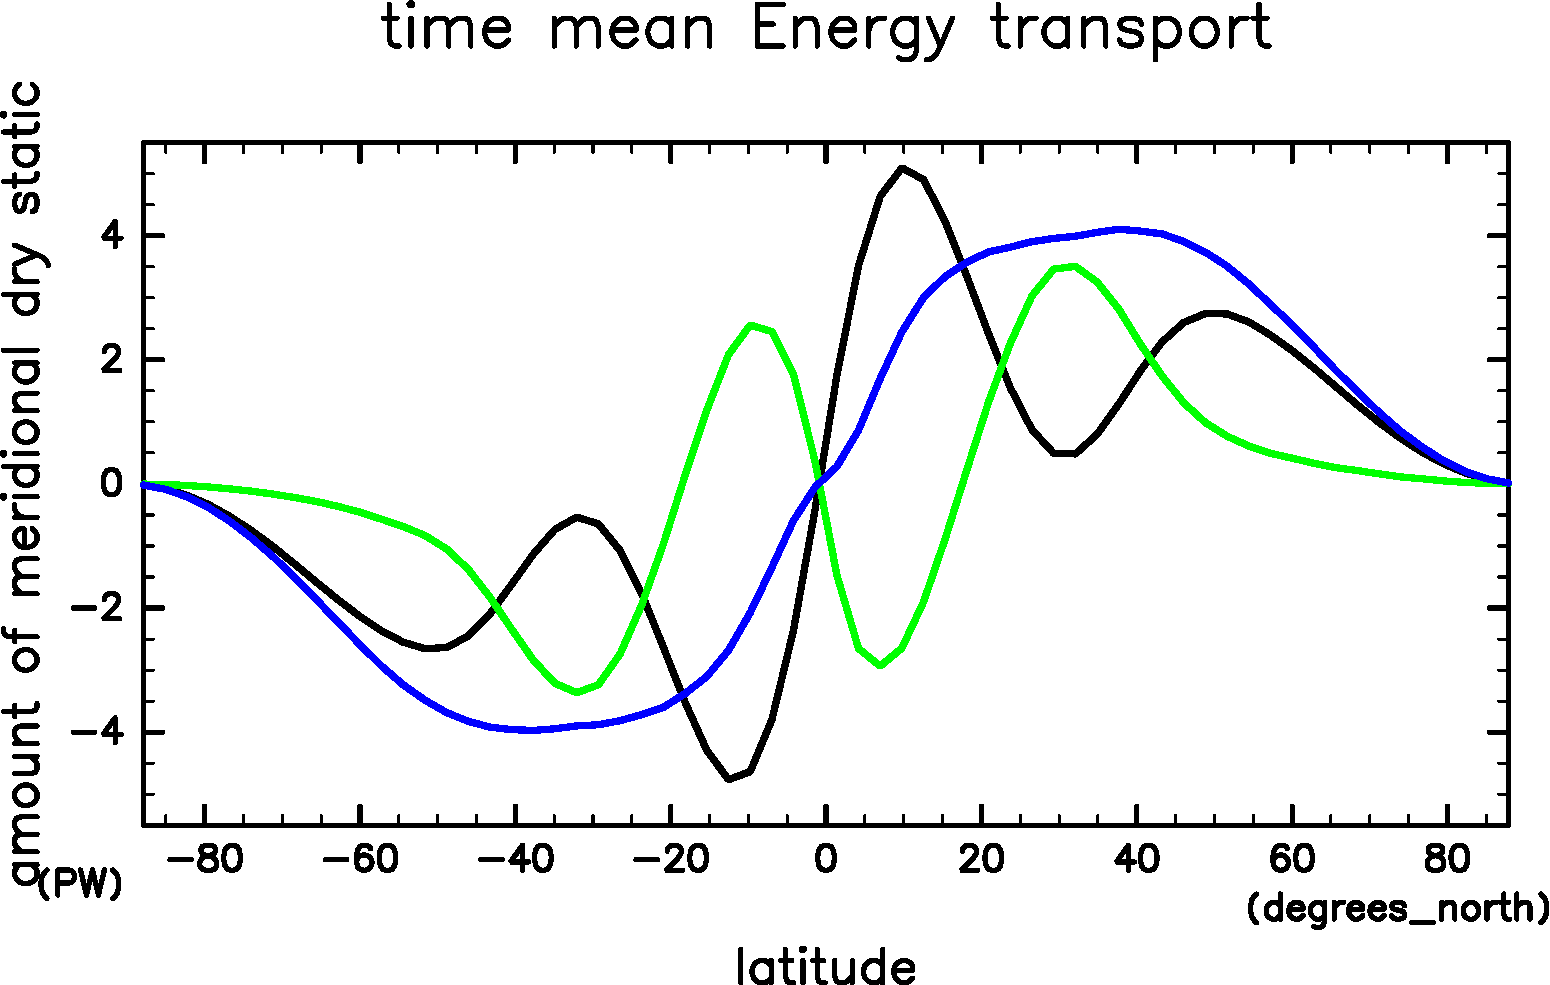
\includegraphics[width=\textwidth]{S1366/EngyFlx,time=14600:14965-crop-rotate.pdf}
		\caption{S1366}\label{EnFlxS1366}
	\end{subfigure}
	\begin{subfigure}{.4\textwidth}
		\centering
		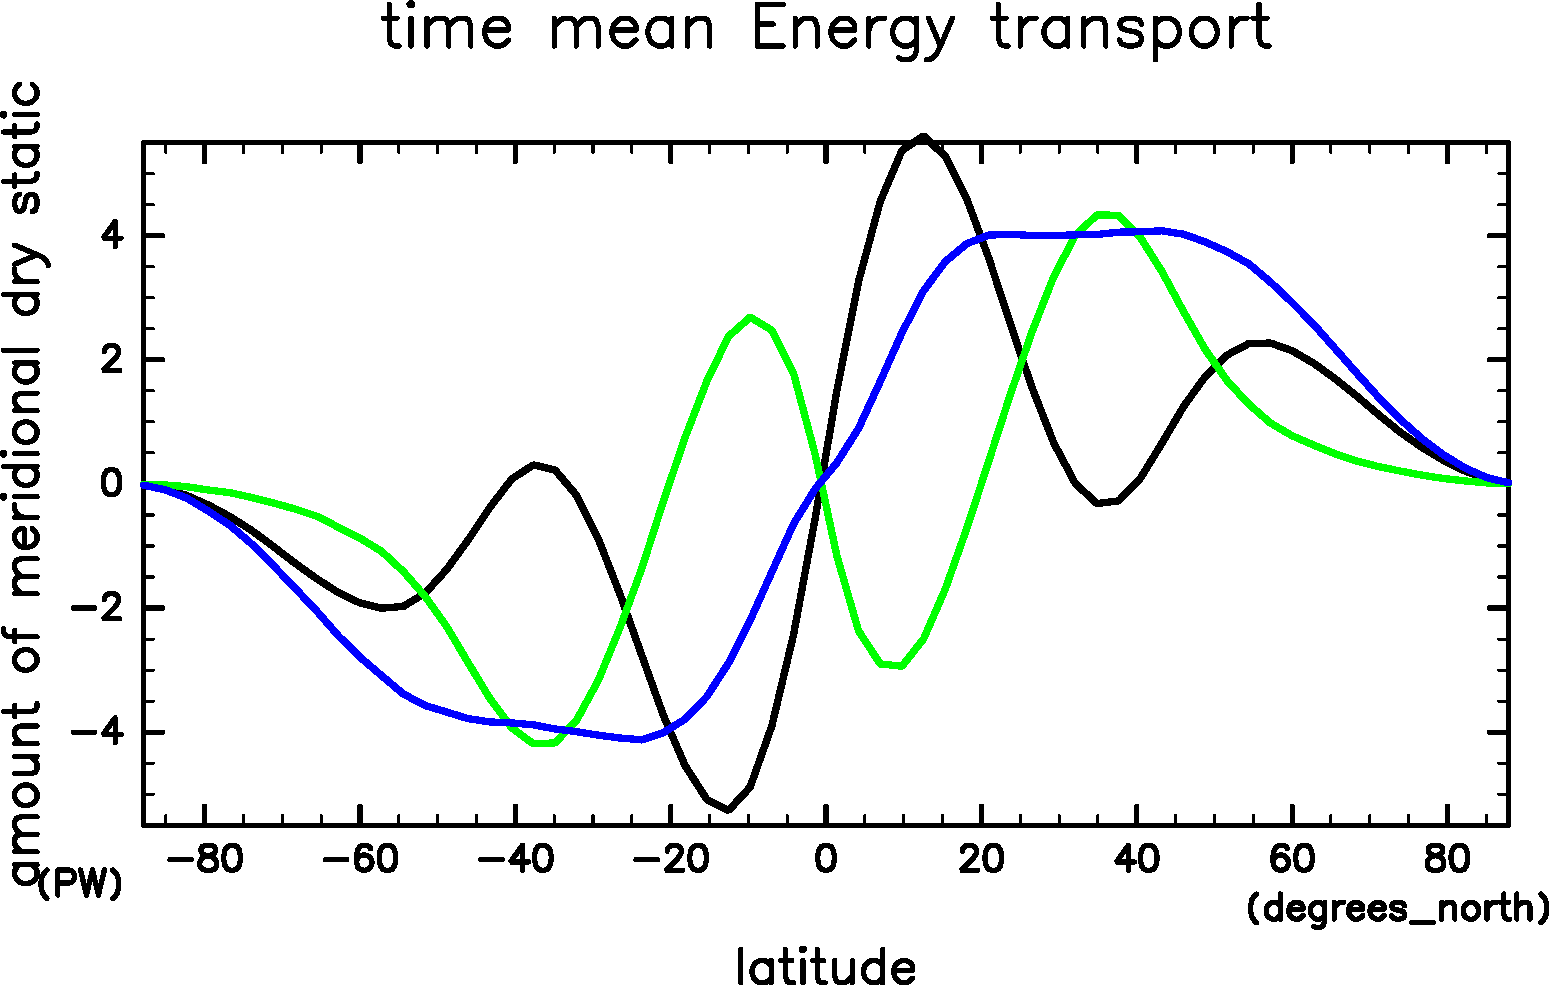
\includegraphics[width=\textwidth]{S1500/EngyFlx,time=3650:4015-crop-rotate.pdf}
		\caption{S1500}\label{EnFlxS1500}
	\end{subfigure}
	\begin{subfigure}{.4\textwidth}
		\centering
		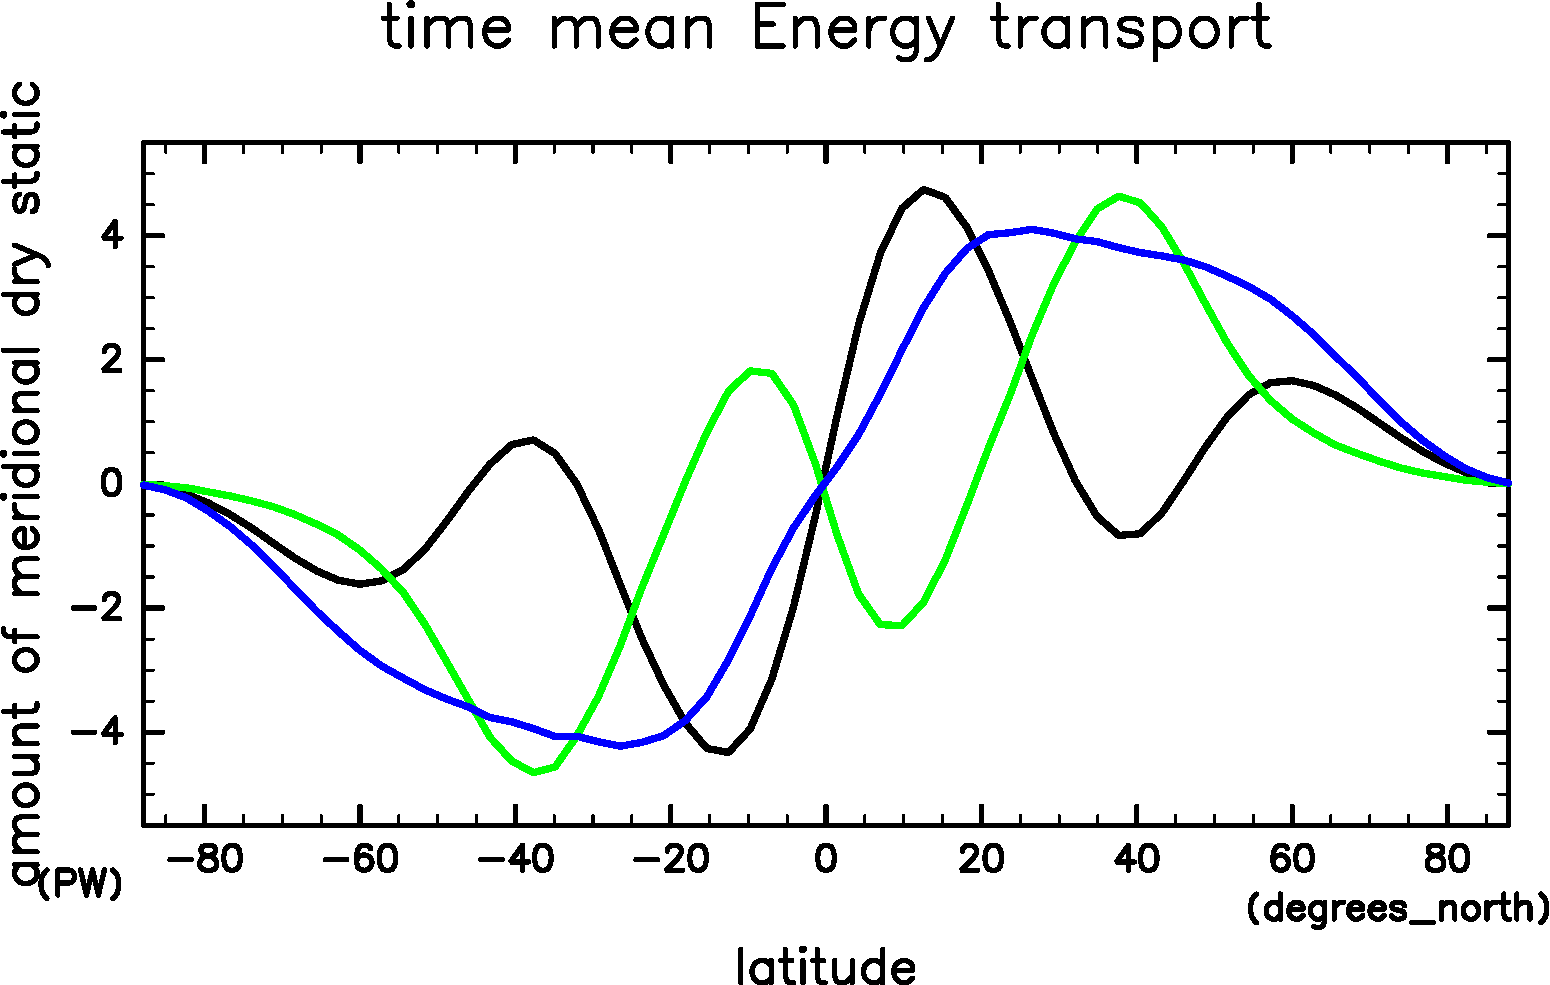
\includegraphics[width=\textwidth]{S1600/EngyFlx,time=3650:4015-crop-rotate.pdf}
		\caption{S1600}\label{EnFlxS1600}
	\end{subfigure}
	\begin{subfigure}{.4\textwidth}
		\centering
		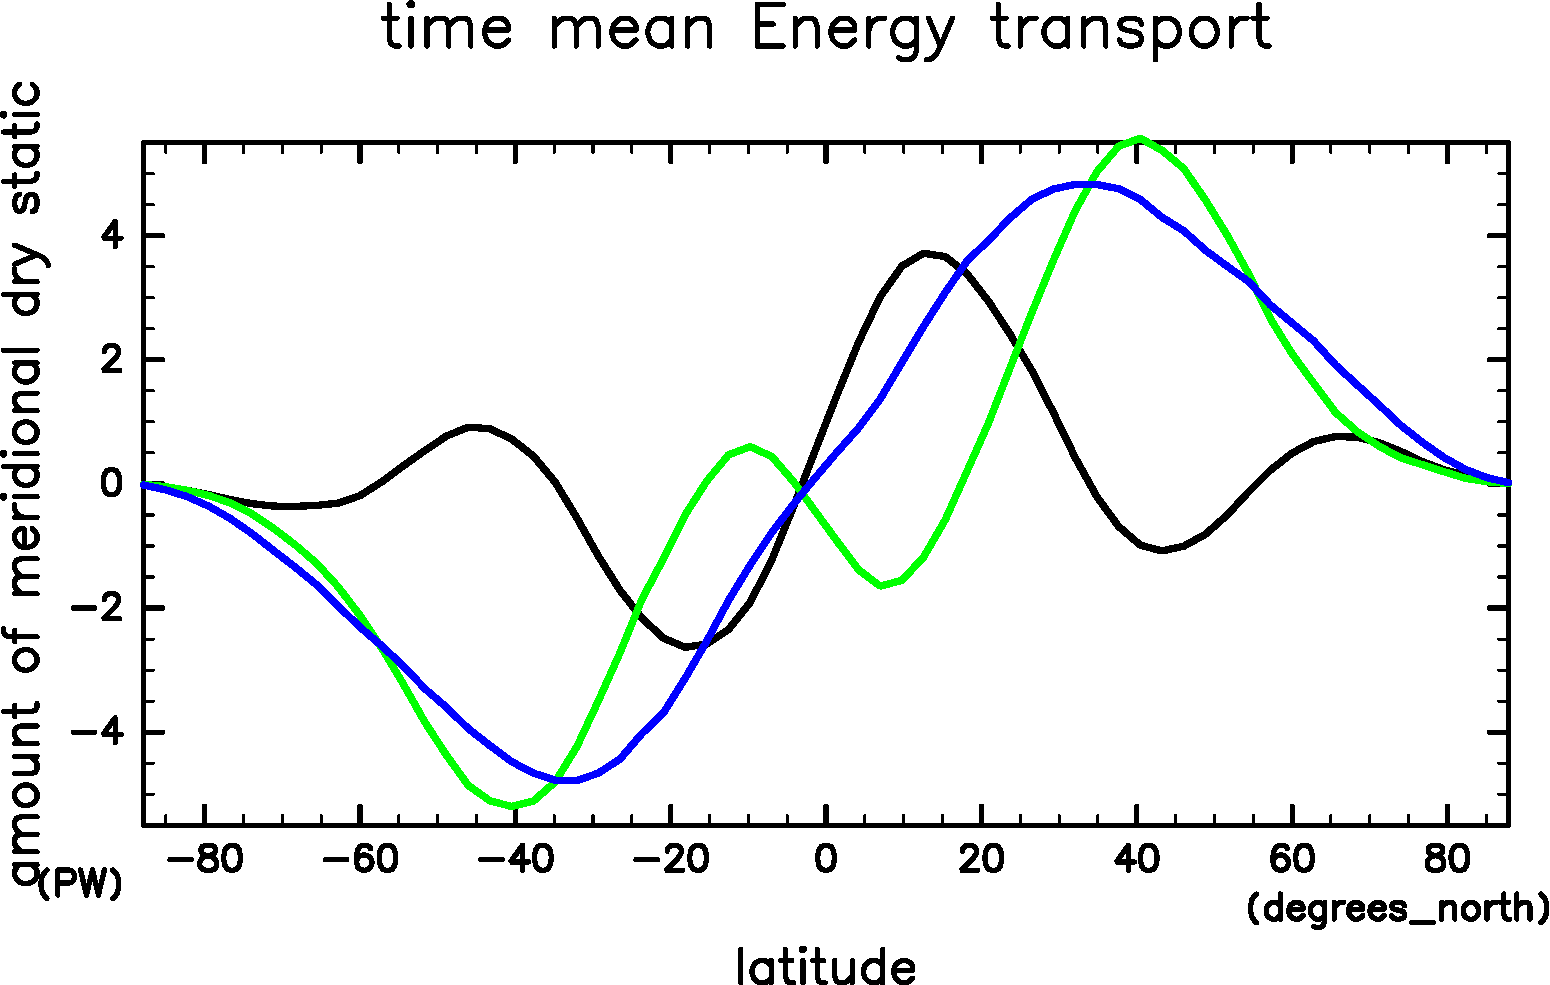
\includegraphics[width=\textwidth]{S1800/EngyFlx,time=3650:4015-crop-rotate.pdf}
		\caption{S1800}\label{EnFlxS1800}
	\end{subfigure}
	\begin{subfigure}{.4\textwidth}
		\centering
		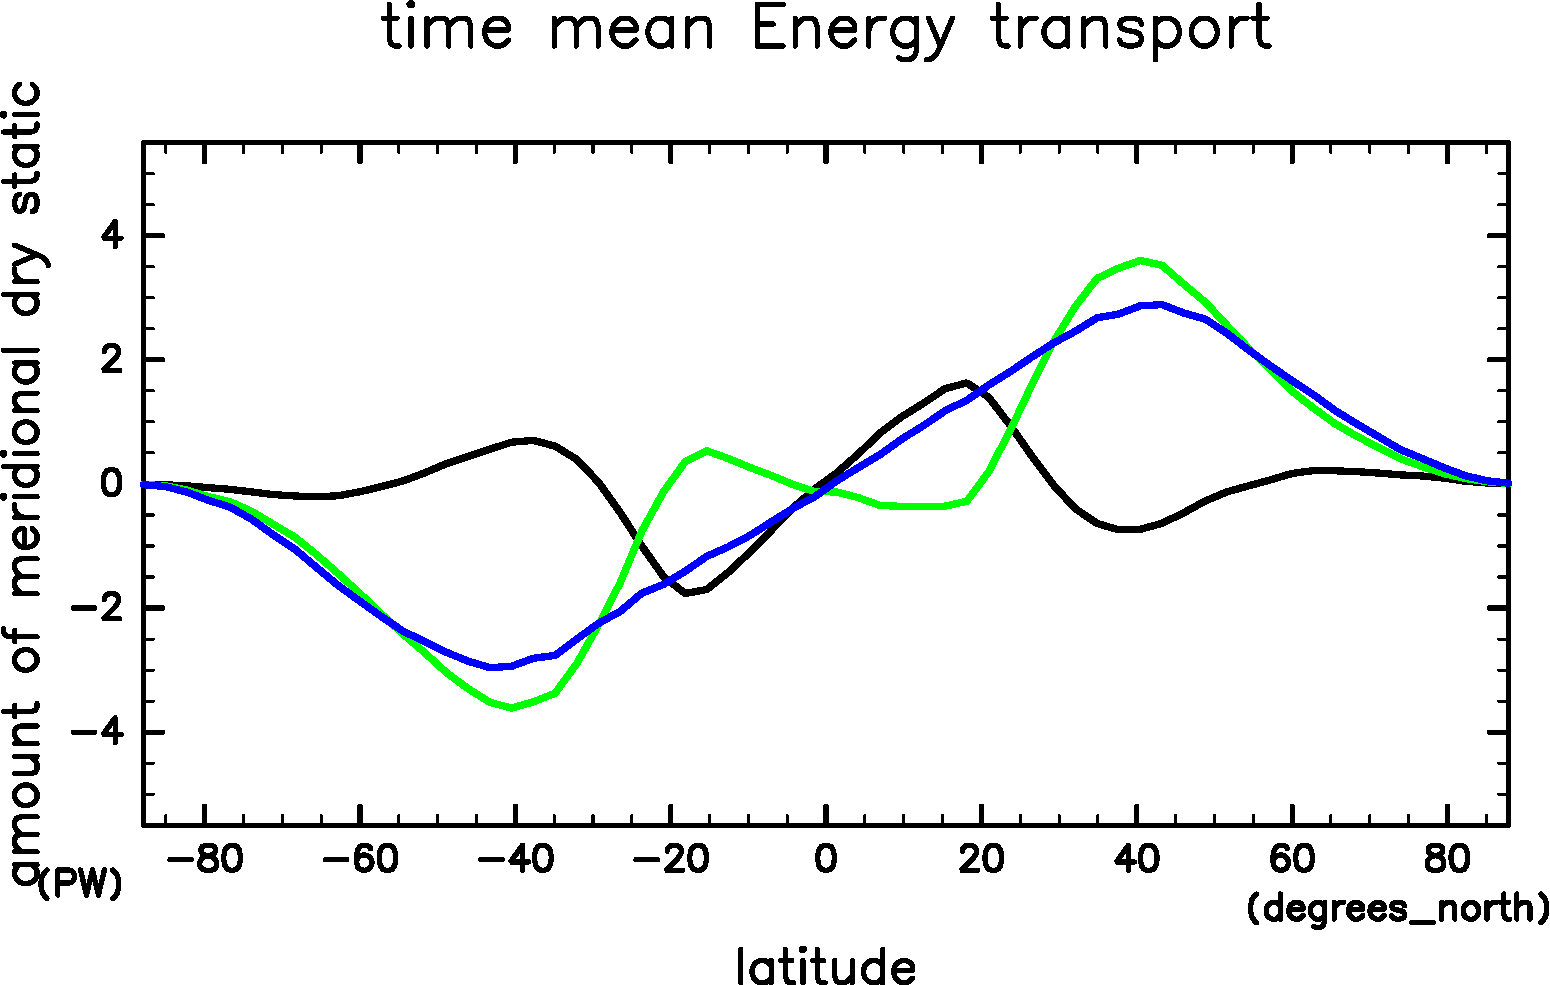
\includegraphics[width=\textwidth]{S2000/EngyFlx,time=7300:7665-crop-rotate.pdf}
		\caption{S2000}\label{EnFlxS2000}
	\end{subfigure}
	\caption[雲あり各実験での南北熱輸送量]{
		雲あり各実験での時間平均・東西平均された南北熱輸送量。
		緑線が潜熱輸送、黒線が乾燥静的エネルギーの輸送、青線が全熱輸送量。
		横軸は緯度であり、縦軸は北向きの輸送量で、単位は \hmu*{PW}。
		\(0.25\) 日間隔で時間平均をとった。
	}\label{EnFlx}
\end{figure}

\begin{figure}[t]
	\centering
	\begin{subfigure}{.4\textwidth}
		\centering
		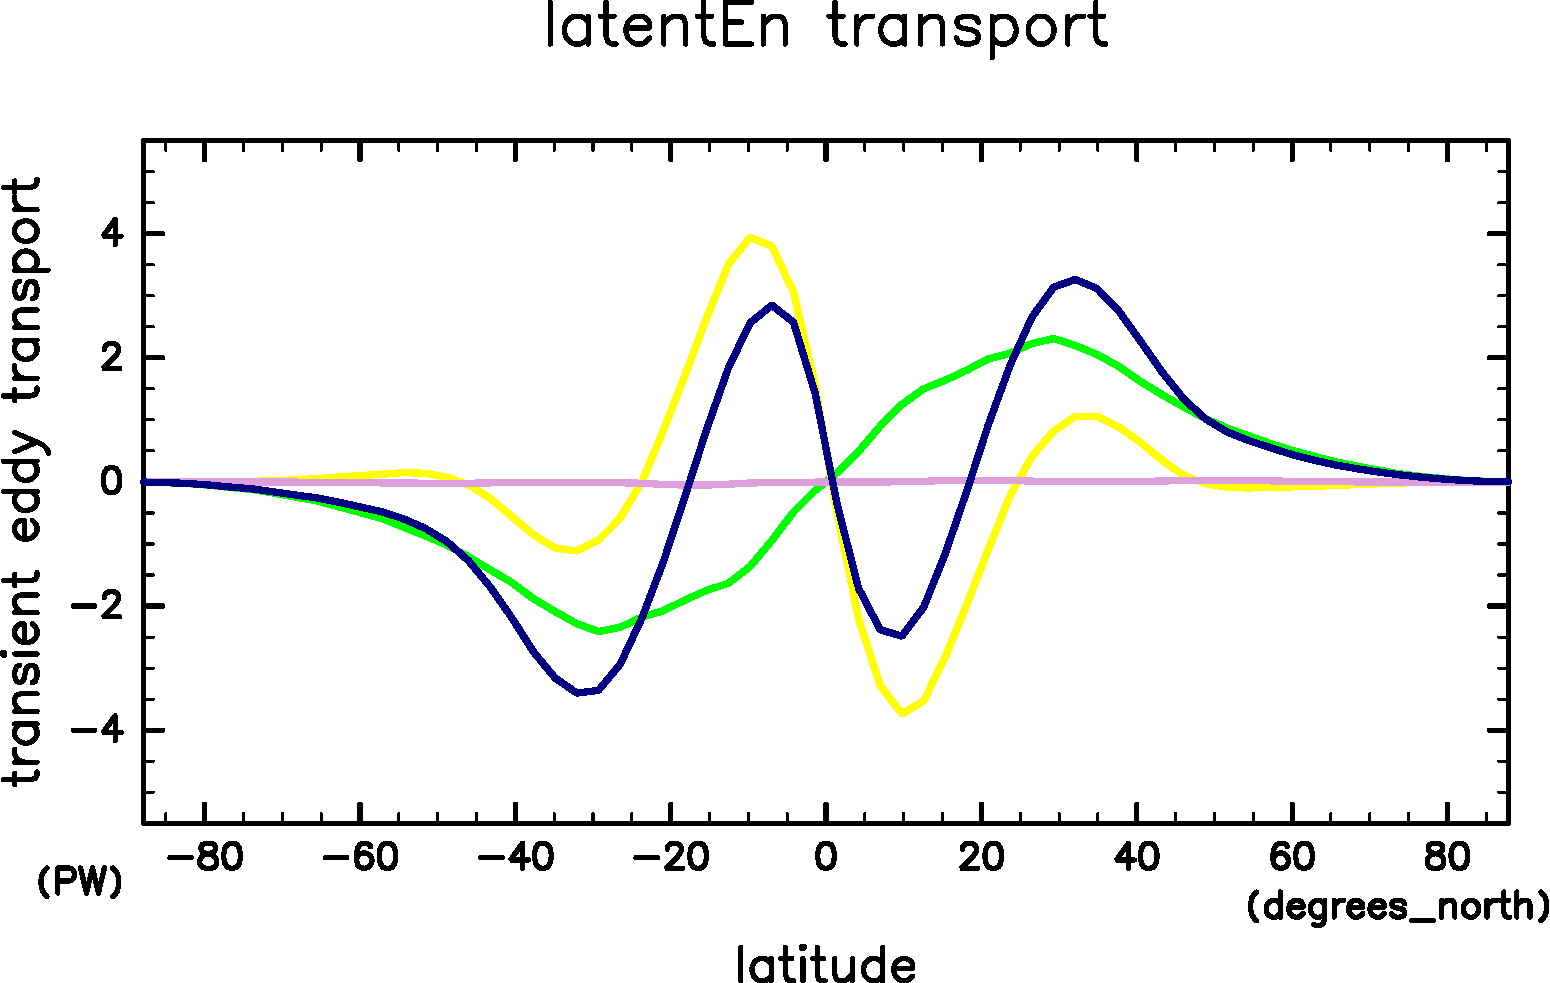
\includegraphics[width=\textwidth]{S1366/MeriHeatTrans@latentEn,time=14600:14965-crop-rotate.pdf}
		\caption{S1366}\label{潜熱S1366}
	\end{subfigure}
	\begin{subfigure}{.4\textwidth}
		\centering
		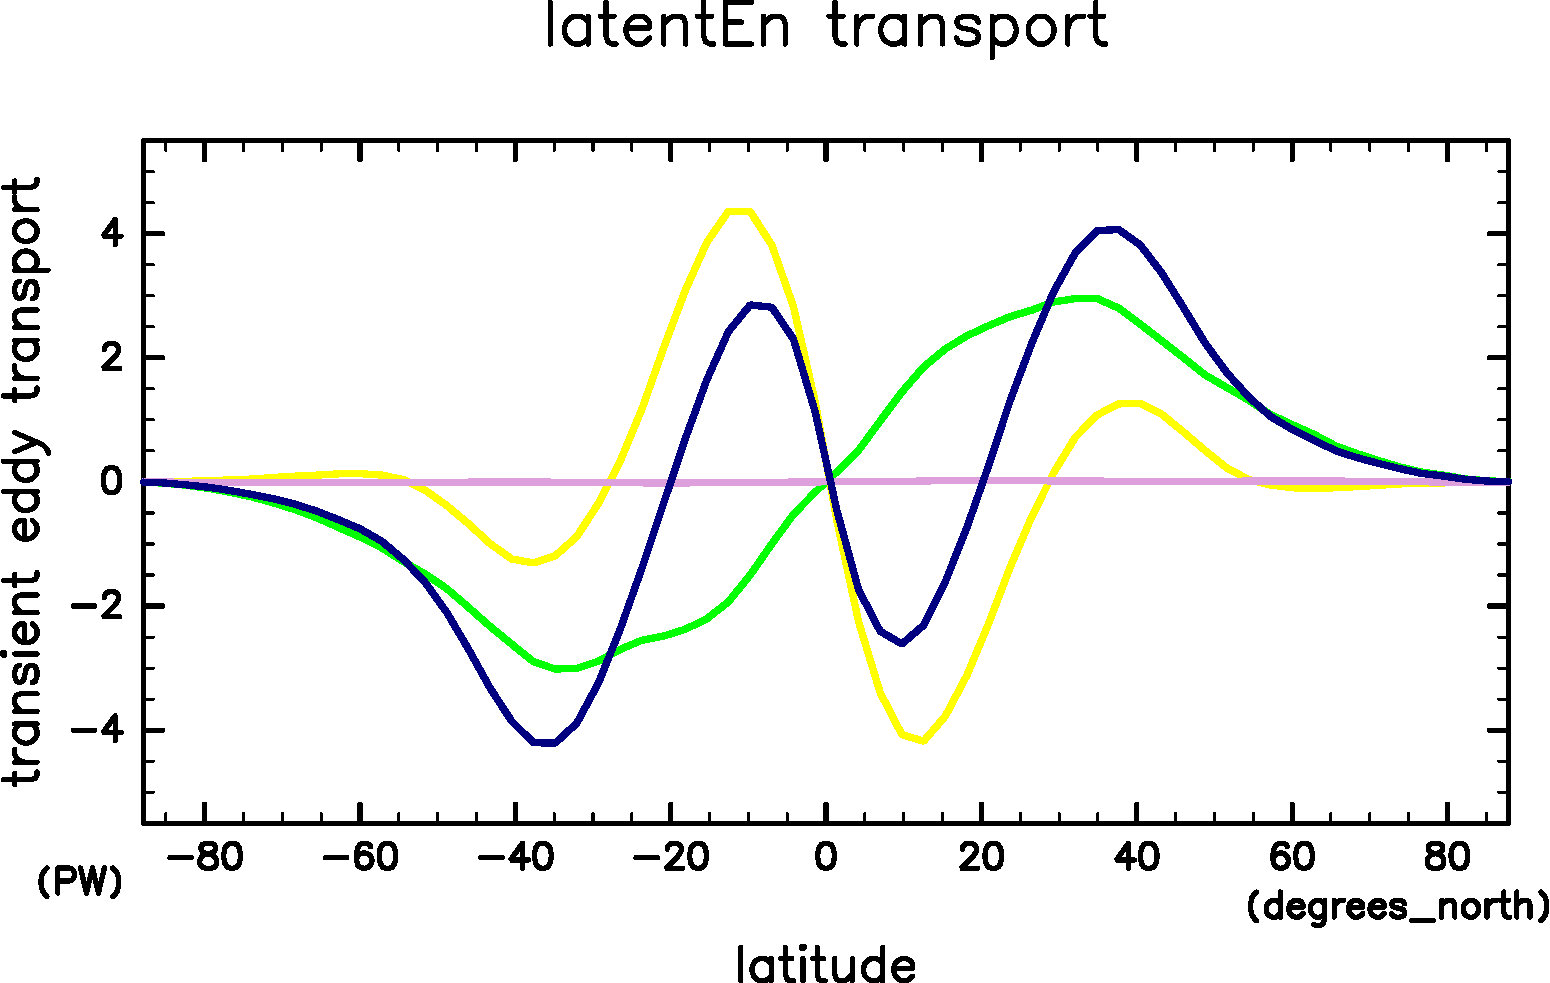
\includegraphics[width=\textwidth]{S1500/MeriHeatTrans@latentEn,time=3650:4015-crop-rotate.pdf}
		\caption{S1500}\label{潜熱S1500}
	\end{subfigure}
	\begin{subfigure}{.4\textwidth}
		\centering
		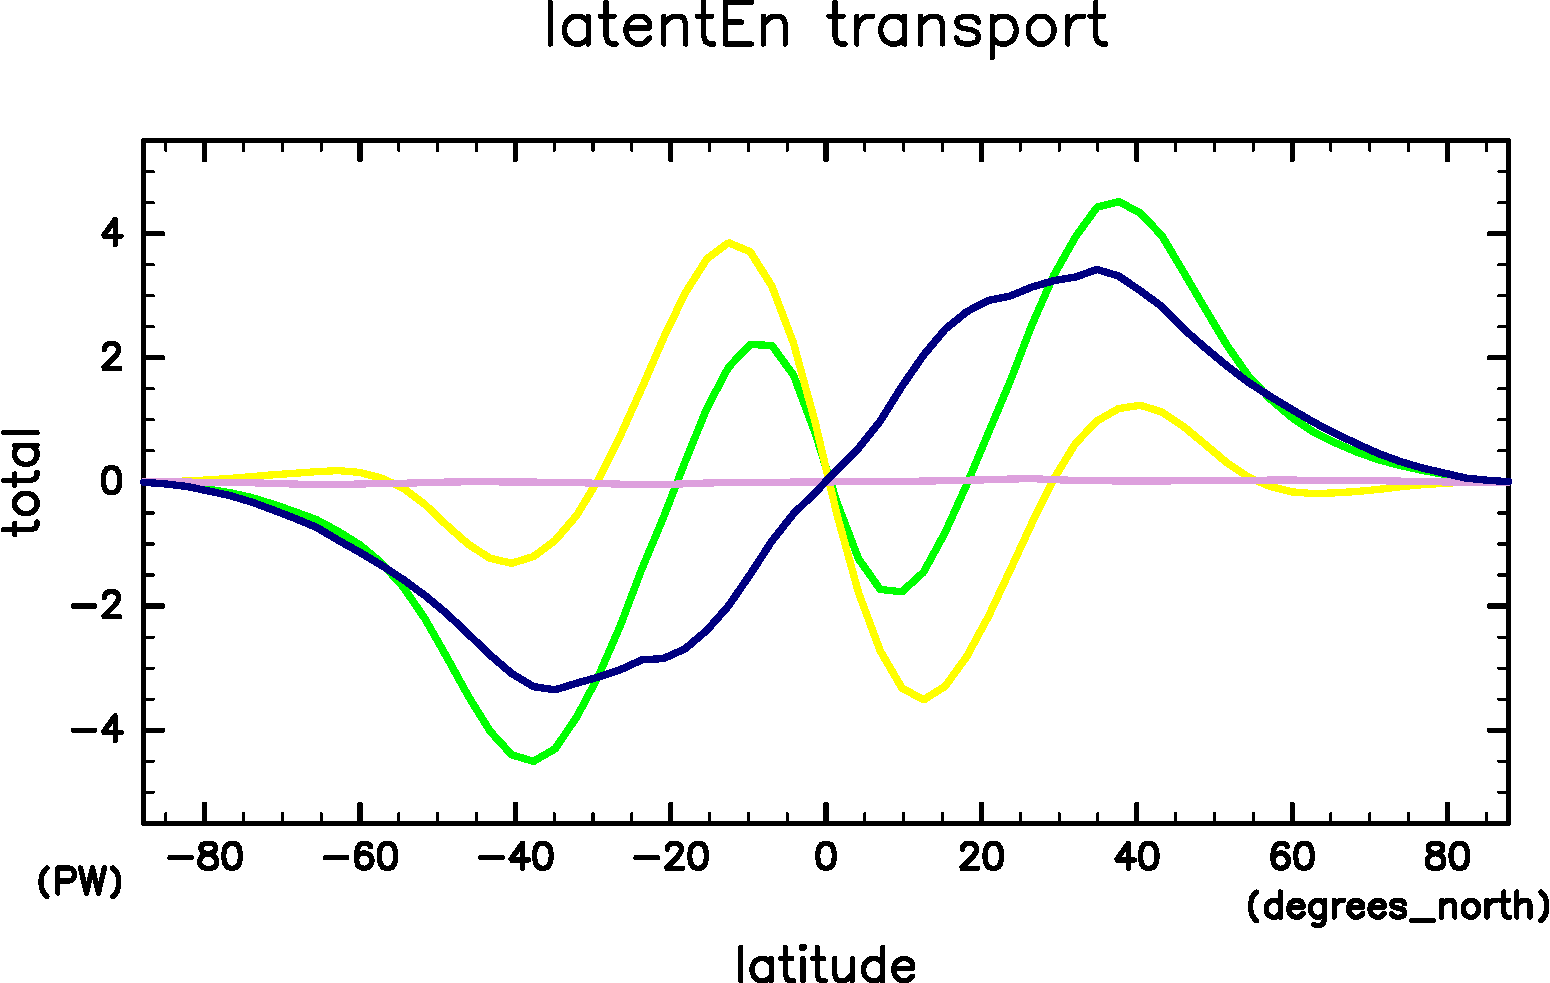
\includegraphics[width=\textwidth]{S1600/MeriHeatTrans@latentEn,time=3650:4015-crop-rotate.pdf}
		\caption{S1600}\label{潜熱S1600}
	\end{subfigure}
	\begin{subfigure}{.4\textwidth}
		\centering
		\includegraphics[width=\textwidth]{S1800/MeriHeatTrans@latentEn,time=3650:4015-crop-rotate.pdf}
		\caption{S1800}\label{潜熱S1800}
	\end{subfigure}
	\begin{subfigure}{.4\textwidth}
		\centering
		\includegraphics[width=\textwidth]{S2000/MeriHeatTrans@latentEn,time=7300:7665-crop-rotate.pdf}
		\caption{S2000}\label{潜熱S2000}
	\end{subfigure}
	\caption[雲あり各実験での潜熱輸送の内訳]{
		雲あり各実験での潜熱輸送。青線が全輸送量 \([\overline{Lqv}]\)、
		黄線が平均子午面循環による輸送量 \([\overline{Lq}][\overline{v}]\)、
		桃線が停滞性擾乱による輸送量 \([\overline{(Lq)^*}\bar v^*]\)、
		緑線が移動性擾乱による輸送量 \([\overline{(Lq)'v'}]\)。
		横軸は緯度であり、縦軸は北向きの輸送量で、単位は \hmu*{PW}。
	}\label{潜熱}
\end{figure}

\begin{figure}[t]
	\centering
	\begin{subfigure}{.4\textwidth}
		\centering
		\includegraphics[width=\textwidth]{S1366/MeriHeatTrans@dryStatEn,time=14600:14965-crop-rotate.pdf}
		\caption{S1366}\label{乾燥静的エネルギーS1366}
	\end{subfigure}
	\begin{subfigure}{.4\textwidth}
		\centering
		\includegraphics[width=\textwidth]{S1500/MeriHeatTrans@dryStatEn,time=3650:4015-crop-rotate.pdf}
		\caption{S1500}\label{乾燥静的エネルギーS1500}
	\end{subfigure}
	\begin{subfigure}{.4\textwidth}
		\centering
		\includegraphics[width=\textwidth]{S1600/MeriHeatTrans@dryStatEn,time=3650:4015-crop-rotate.pdf}
		\caption{S1600}\label{乾燥静的エネルギーS1600}
	\end{subfigure}
	\begin{subfigure}{.4\textwidth}
		\centering
		\includegraphics[width=\textwidth]{S1800/MeriHeatTrans@dryStatEn,time=3650:4015-crop-rotate.pdf}
		\caption{S1800}\label{乾燥静的エネルギーS1800}
	\end{subfigure}
	\begin{subfigure}{.4\textwidth}
		\centering
		\includegraphics[width=\textwidth]{S2000/MeriHeatTrans@dryStatEn,time=7300:7665-crop-rotate.pdf}
		\caption{S2000}\label{乾燥静的エネルギーS2000}
	\end{subfigure}
	\caption[雲あり各実験での乾燥静的エネルギー輸送の内訳]{
		雲あり各実験での潜熱輸送。青線が全輸送量 \([\overline{(c_{pn}T+gz)v}]\)、
		黄線が平均子午面循環による輸送量 \([\overline{c_{pn}T+gz}][\overline{v}]\)、
		桃線が停滞性擾乱による輸送量 \([\overline{(c_{pn}T+gz)^*}\bar v^*]\)、
		緑線が移動性擾乱による輸送量 \([\overline{(c_{pn}T+gz)'v'}]\)。
		横軸は緯度であり、縦軸は北向きの輸送量で、単位は \hmu*{PW}。
	}\label{乾燥静的エネルギー}
\end{figure}

\afterpage{\clearpage}

図 \ref{潜熱平均子午面循環} に潜熱の平均子午面循環による輸送の子午面分布、
すなわち \([\overline{Lq}][\bar v]\) の子午面分布を示す。
また、図 \ref{Lq} に \([\overline{Lq}]\) の子午面分布も示す。
地表面付近では比湿が大きい(図 \ref{S1366比湿} から \ref{S2000比湿})ので、
\([\overline{Lq}]\) の値も大きくなり、
地表面付近で平均子午面循環に依る潜熱の輸送が大きいことがわかる。
地表面付近の低緯度で高緯度向きの輸送があり、太陽定数が大きくなると
その量が大きくなる。

図 \ref{潜熱移動性擾乱} に潜熱の移動性擾乱による輸送の子午面分布、
すなわち \([\overline{(Lq)^*}\bar{v^*}]\) の子午面分布を示す。
中緯度域で移動性擾乱による輸送が大きいことがわかる。
輸送が大きくなっている高度は、太陽定数が増大するにつれて上昇している。
輸送が大きくなっている箇所では、傾圧不安定によって熱が輸送されている。

図 \ref{潜熱停滞性擾乱} に潜熱の停滞性擾乱による輸送の子午面分布、
すなわち \([\overline{(Lq)'v'}]\) の子午面分布を示す。
潜熱の停滞性擾乱による輸送は、平均子午面循環による輸送や、
移動性擾乱による輸送と比べて値が小さく、特に輸送が大きくなっている領域がない。
これは、モデルに地形が含まれていないため、停滞性擾乱がほとんど発生していない
ことが理由だと考えられる。

\begin{figure}[t]
	\centering
	\begin{subfigure}{.4\textwidth}
		\centering
		\includegraphics[width=\textwidth]{S1366/Lq,time=14600:14965-crop-rotate.pdf}
		\caption{S1366}\label{LqS1366}
	\end{subfigure}
	\begin{subfigure}{.4\textwidth}
		\centering
		\includegraphics[width=\textwidth]{S1500/Lq,time=3650:4015-crop-rotate.pdf}
		\caption{S1500}\label{LqS1500}
	\end{subfigure}
	\begin{subfigure}{.4\textwidth}
		\centering
		\includegraphics[width=\textwidth]{S1600/Lq,time=3650:4015-crop-rotate.pdf}
		\caption{S1600}\label{LqS1600}
	\end{subfigure}
	\begin{subfigure}{.4\textwidth}
		\centering
		\includegraphics[width=\textwidth]{S1800/Lq,time=3650:4015-crop-rotate.pdf}
		\caption{S1800}\label{LqS1800}
	\end{subfigure}
	\begin{subfigure}{.4\textwidth}
		\centering
		\includegraphics[width=\textwidth]{S2000/Lq,time=7300:7665-crop-rotate.pdf}
		\caption{S2000}\label{LqS2000}
	\end{subfigure}
	\caption[雲あり各実験での潜熱の子午面分布]{
		雲あり各実験での潜熱 \([\overline{Lq}]\) の子午面分布。
		等値線間隔は全て \(25\hmu{KJ}\) である。
	}\label{Lq}
\end{figure}

\begin{figure}[t]
	\centering
	\begin{subfigure}{.4\textwidth}
		\centering
		\includegraphics[width=\textwidth]{S1366/MeriHeatTransTest@latentEn_M,time=14600:14965-crop-rotate.pdf}
		\caption{S1366}\label{潜熱平均子午面循環S1366}
	\end{subfigure}
	\begin{subfigure}{.4\textwidth}
		\centering
		\includegraphics[width=\textwidth]{S1500/MeriHeatTransTest@latentEn_M,time=3650:4015-crop-rotate.pdf}
		\caption{S1500}\label{潜熱平均子午面循環S1500}
	\end{subfigure}
	\begin{subfigure}{.4\textwidth}
		\centering
		\includegraphics[width=\textwidth]{S1600/MeriHeatTransTest@latentEn_M,time=3650:4015-crop-rotate.pdf}
		\caption{S1600}\label{潜熱平均子午面循環S1600}
	\end{subfigure}
	\begin{subfigure}{.4\textwidth}
		\centering
		\includegraphics[width=\textwidth]{S1800/MeriHeatTransTest@latentEn_M,time=3650:4015-crop-rotate.pdf}
		\caption{S1800}\label{潜熱平均子午面循環S1800}
	\end{subfigure}
	\begin{subfigure}{.4\textwidth}
		\centering
		\includegraphics[width=\textwidth]{S2000/MeriHeatTransTest@latentEn_M,time=7300:7665-crop-rotate.pdf}
		\caption{S2000}\label{潜熱平均子午面循環S2000}
	\end{subfigure}
	\caption[雲あり各実験での平均子午面循環による潜熱輸送の子午面分布]{
		雲あり各実験での平均子午面循環による潜熱輸送 \([\overline{Lq}][\bar v]\) の子午面分布。
		等値線間隔は全て \(15\hmu{PW}\) である。
	}\label{潜熱平均子午面循環}
\end{figure}

\begin{figure}[t]
	\centering
	\begin{subfigure}{.4\textwidth}
		\centering
		\includegraphics[width=\textwidth]{S1366/MeriHeatTransTest@latentEn_TE,time=14600:14965-crop-rotate.pdf}
		\caption{S1366}\label{潜熱移動性擾乱S1366}
	\end{subfigure}
	\begin{subfigure}{.4\textwidth}
		\centering
		\includegraphics[width=\textwidth]{S1500/MeriHeatTransTest@latentEn_TE,time=3650:4015-crop-rotate.pdf}
		\caption{S1500}\label{潜熱移動性擾乱S1500}
	\end{subfigure}
	\begin{subfigure}{.4\textwidth}
		\centering
		\includegraphics[width=\textwidth]{S1600/MeriHeatTransTest@latentEn_TE,time=3650:4015-crop-rotate.pdf}
		\caption{S1600}\label{潜熱移動性擾乱S1600}
	\end{subfigure}
	\begin{subfigure}{.4\textwidth}
		\centering
		\includegraphics[width=\textwidth]{S1800/MeriHeatTransTest@latentEn_TE,time=3650:4015-crop-rotate.pdf}
		\caption{S1800}\label{潜熱移動性擾乱S1800}
	\end{subfigure}
	\begin{subfigure}{.4\textwidth}
		\centering
		\includegraphics[width=\textwidth]{S2000/MeriHeatTransTest@latentEn_TE,time=7300:7665-crop-rotate.pdf}
		\caption{S2000}\label{潜熱移動性擾乱S2000}
	\end{subfigure}
	\caption[雲あり各実験での移動性擾乱による潜熱輸送の子午面分布]{
		雲あり各実験での移動性擾乱による潜熱輸送 \([\overline{(Lq)'v'}]\) の子午面分布。
		等値線間隔は全て \(1\hmu{PW}\) である。
	}\label{潜熱移動性擾乱}
\end{figure}

\begin{figure}[t]
	\centering
	\begin{subfigure}{.4\textwidth}
		\centering
		\includegraphics[width=\textwidth]{S1366/MeriHeatTransTest@latentEn_SE,time=14600:14965-crop-rotate.pdf}
		\caption{S1366}\label{潜熱停滞性擾乱S1366}
	\end{subfigure}
	\begin{subfigure}{.4\textwidth}
		\centering
		\includegraphics[width=\textwidth]{S1500/MeriHeatTransTest@latentEn_SE,time=3650:4015-crop-rotate.pdf}
		\caption{S1500}\label{潜熱停滞性擾乱S1500}
	\end{subfigure}
	\begin{subfigure}{.4\textwidth}
		\centering
		\includegraphics[width=\textwidth]{S1600/MeriHeatTransTest@latentEn_SE,time=3650:4015-crop-rotate.pdf}
		\caption{S1600}\label{潜熱停滞性擾乱S1600}
	\end{subfigure}
	\begin{subfigure}{.4\textwidth}
		\centering
		\includegraphics[width=\textwidth]{S1800/MeriHeatTransTest@latentEn_SE,time=3650:4015-crop-rotate.pdf}
		\caption{S1800}\label{潜熱停滞性擾乱S1800}
	\end{subfigure}
	\begin{subfigure}{.4\textwidth}
		\centering
		\includegraphics[width=\textwidth]{S2000/MeriHeatTransTest@latentEn_SE,time=7300:7665-crop-rotate.pdf}
		\caption{S2000}\label{潜熱停滞性擾乱S2000}
	\end{subfigure}
	\caption[雲あり各実験でのに停滞性擾乱による潜熱輸送の子午面分布]{
		雲あり各実験での停滞性擾乱による潜熱輸送 \([\overline{(Lq)^*}\bar v^*]\) の子午面分布。
		等値線間隔は全て \(0.1\hmu{PW}\) である。
	}\label{潜熱停滞性擾乱}
\end{figure}

\afterpage{\clearpage}

図 \ref{乾燥静的エネルギー平均子午面循環} に乾燥静的エネルギーの
平均子午面循環による輸送の子午面分布、すなわち 
\([\overline{(c_{pn}T+gz)}][\bar v]\) の子午面分布を示す。
また、図 \ref{Cp+gz} に \([\overline{(c_{pn}T+gz)}]\) の子午面分布を示す。
いずれの実験でも、地表面付近の低緯度で低緯度向きの輸送があり、
地表面付近の中緯度で高緯度向きの
輸送がある。また、低緯度の高高度で高緯度向きの輸送がある。
地表面付近の輸送は太陽定数が大きくなると小さくなり、
上空での輸送の高度は太陽定数が大きくなると上昇する。
上空で輸送が大きくなっている高度が高くなるのは、太陽定数が増大すると
ハドレー循環の高度が高くなるからである。

図 \ref{乾燥静的エネルギー移動性擾乱} に乾燥静的エネルギーの移動性擾乱による
輸送の子午面分布、すなわち \([\overline{(c_{pn}T+gz)^*}\bar{v^*}]\) の子午面分布を示す。
中緯度域で輸送量が大きくなっている。
輸送が大きくなっている高度は、太陽定数が増大するにつれて上昇しているのがわかる。
輸送が大きくなっている箇所では、傾圧不安定によって熱が輸送されている。

図 \ref{乾燥静的エネルギー停滞性擾乱} に乾燥静的エネルギーの停滞性擾乱による輸送の子午面分布、
すなわち \([\overline{(c_{pn}T+gz)'v'}]\) の子午面分布を示す。
乾燥静的エネルギーの停滞性擾乱による輸送は、平均子午面循環による輸送や、
移動性擾乱による輸送と比べて値が小さく、特に輸送が大きくなっている領域がない。
これは、モデルに地形が含まれていないため、停滞性擾乱がほとんど発生していない
ことが理由だと考えられる。

\begin{figure}[t]
	\centering
	\begin{subfigure}{.4\textwidth}
		\centering
		\includegraphics[width=\textwidth]{S1366/CpT+gz,time=14600:14965-crop-rotate.pdf}
		\caption{S1366}\label{CpT+gzS1366}
	\end{subfigure}
	\begin{subfigure}{.4\textwidth}
		\centering
		\includegraphics[width=\textwidth]{S1500/CpT+gz,time=3650:4015-crop-rotate.pdf}
		\caption{S1500}\label{CpT+gzS1500}
	\end{subfigure}
	\begin{subfigure}{.4\textwidth}
		\centering
		\includegraphics[width=\textwidth]{S1600/CpT+gz,time=3650:4015-crop-rotate.pdf}
		\caption{S1600}\label{CpT+gzS1600}
	\end{subfigure}
	\begin{subfigure}{.4\textwidth}
		\centering
		\includegraphics[width=\textwidth]{S1800/CpT+gz,time=3650:4015-crop-rotate.pdf}
		\caption{S1800}\label{CpT+gzS1800}
	\end{subfigure}
	\begin{subfigure}{.4\textwidth}
		\centering
		\includegraphics[width=\textwidth]{S2000/CpT+gz,time=7300:7665-crop-rotate.pdf}
		\caption{S2000}\label{CpT+gzS2000}
	\end{subfigure}
	\caption[雲あり各実験での乾燥静的エネルギーの子午面分布]{
		雲あり各実験での乾燥静的エネルギー \([\overline{c_{pn}T+gz}]\)の子午面分布。
		等値線間隔は全て \(25\hmu{KJ}\) である。
	}\label{Cp+gz}
\end{figure}

\begin{figure}[t]
	\centering
	\begin{subfigure}{.4\textwidth}
		\centering
		\includegraphics[width=\textwidth]{S1366/MeriHeatTransTest@dryStatEn_M,time=14600:14965-crop-rotate.pdf}
		\caption{S1366}\label{乾燥静的エネルギー平均子午面循環S1366}
	\end{subfigure}
	\begin{subfigure}{.4\textwidth}
		\centering
		\includegraphics[width=\textwidth]{S1500/MeriHeatTransTest@dryStatEn_M,time=3650:4015-crop-rotate.pdf}
		\caption{S1500}\label{乾燥静的エネルギー平均子午面循環S1500}
	\end{subfigure}
	\begin{subfigure}{.4\textwidth}
		\centering
		\includegraphics[width=\textwidth]{S1600/MeriHeatTransTest@dryStatEn_M,time=3650:4015-crop-rotate.pdf}
		\caption{S1600}\label{乾燥静的エネルギー平均子午面循環S1600}
	\end{subfigure}
	\begin{subfigure}{.4\textwidth}
		\centering
		\includegraphics[width=\textwidth]{S1800/MeriHeatTransTest@dryStatEn_M,time=3650:4015-crop-rotate.pdf}
		\caption{S1800}\label{乾燥静的エネルギー平均子午面循環S1800}
	\end{subfigure}
	\begin{subfigure}{.4\textwidth}
		\centering
		\includegraphics[width=\textwidth]{S2000/MeriHeatTransTest@dryStatEn_M,time=7300:7665-crop-rotate.pdf}
		\caption{S2000}\label{乾燥静的エネルギー平均子午面循環S2000}
	\end{subfigure}
	\caption[雲あり各実験での平均子午面循環による乾燥静的エネルギー輸送の子午面分布]{
		雲あり各実験での平均子午面循環による乾燥静的エネルギー輸送 \([\overline{(c_{pn}T+gz)}][\bar v]\) の子午面分布。
		等値線間隔は全て \(60\hmu{PW}\) である。
	}\label{乾燥静的エネルギー平均子午面循環}
\end{figure}

\begin{figure}[t]
	\centering
	\begin{subfigure}{.4\textwidth}
		\centering
		\includegraphics[width=\textwidth]{S1366/MeriHeatTransTest@dryStatEn_TE,time=14600:14965-crop-rotate.pdf}
		\caption{S1366}\label{乾燥静的エネルギー移動性擾乱S1366}
	\end{subfigure}
	\begin{subfigure}{.4\textwidth}
		\centering
		\includegraphics[width=\textwidth]{S1500/MeriHeatTransTest@dryStatEn_TE,time=3650:4015-crop-rotate.pdf}
		\caption{S1500}\label{乾燥静的エネルギー移動性擾乱S1500}
	\end{subfigure}
	\begin{subfigure}{.4\textwidth}
		\centering
		\includegraphics[width=\textwidth]{S1600/MeriHeatTransTest@dryStatEn_TE,time=3650:4015-crop-rotate.pdf}
		\caption{S1600}\label{乾燥静的エネルギー移動性擾乱S1600}
	\end{subfigure}
	\begin{subfigure}{.4\textwidth}
		\centering
		\includegraphics[width=\textwidth]{S1800/MeriHeatTransTest@dryStatEn_TE,time=3650:4015-crop-rotate.pdf}
		\caption{S1800}\label{乾燥静的エネルギー移動性擾乱S1800}
	\end{subfigure}
	\begin{subfigure}{.4\textwidth}
		\centering
		\includegraphics[width=\textwidth]{S2000/MeriHeatTransTest@dryStatEn_TE,time=7300:7665-crop-rotate.pdf}
		\caption{S2000}\label{乾燥静的エネルギー移動性擾乱S2000}
	\end{subfigure}
	\caption[雲あり各実験での移動性擾乱に依る乾燥静的エネルギー輸送の子午面分布]{
		雲あり各実験での移動性擾乱による乾燥静的エネルギー輸送 \([\overline{(c_{pn}T+gz)^*}\bar{v^*}]\) の子午面分布。
		等値線間隔は全て \(1\hmu{PW}\) である。
	}\label{乾燥静的エネルギー移動性擾乱}
\end{figure}

\begin{figure}[t]
	\centering
	\begin{subfigure}{.4\textwidth}
		\centering
		\includegraphics[width=\textwidth]{S1366/MeriHeatTransTest@dryStatEn_SE,time=14600:14965-crop-rotate.pdf}
		\caption{S1366}\label{乾燥静的エネルギー停滞性擾乱S1366}
	\end{subfigure}
	\begin{subfigure}{.4\textwidth}
		\centering
		\includegraphics[width=\textwidth]{S1500/MeriHeatTransTest@dryStatEn_SE,time=3650:4015-crop-rotate.pdf}
		\caption{S1500}\label{乾燥静的エネルギー停滞性擾乱S1500}
	\end{subfigure}
	\begin{subfigure}{.4\textwidth}
		\centering
		\includegraphics[width=\textwidth]{S1600/MeriHeatTransTest@dryStatEn_SE,time=3650:4015-crop-rotate.pdf}
		\caption{S1600}\label{乾燥静的エネルギー停滞性擾乱S1600}
	\end{subfigure}
	\begin{subfigure}{.4\textwidth}
		\centering
		\includegraphics[width=\textwidth]{S1800/MeriHeatTransTest@dryStatEn_SE,time=3650:4015-crop-rotate.pdf}
		\caption{S1800}\label{乾燥静的エネルギー停滞性擾乱S1800}
	\end{subfigure}
	\begin{subfigure}{.4\textwidth}
		\centering
		\includegraphics[width=\textwidth]{S2000/MeriHeatTransTest@dryStatEn_SE,time=7300:7665-crop-rotate.pdf}
		\caption{S2000}\label{乾燥静的エネルギー停滞性擾乱S2000}
	\end{subfigure}
	\caption[雲あり各実験でのに停滞性擾乱依る乾燥静的エネルギー輸送の子午面分布]{
		雲あり各実験での停滞性擾乱による乾燥静的エネルギー輸送 \([\overline{(c_{pn}T+gz)'v'}]\) の子午面分布。
		等値線間隔は全て \(0.1\hmu{PW}\) である。
	}\label{乾燥静的エネルギー停滞性擾乱}
\end{figure}

\afterpage{\clearpage}

図 \ref{EnFlx南北分布} に熱収支の緯度分布を示す。
太陽定数が大きくなるにつれて、地表面の正味フラックスが減少し、
凝結加熱率と蒸発フラックスが大きくなっているのがわかる。
すなわち、太陽定数が大きくなるにつれて、入射量のほとんど全てが
潜熱フラックスの形で大気に供給される。

\begin{figure}[t]
	\centering
	\begin{subfigure}{.4\textwidth}
		\centering
		\includegraphics[width=\textwidth]{S1366/HeatFlx,time=14600:14965-crop-rotate.pdf}
		\caption{S1366}\label{EnFlx南北分布S1366}
	\end{subfigure}
	\begin{subfigure}{.4\textwidth}
		\centering
		\includegraphics[width=\textwidth]{S1500/HeatFlx,time=3650:4015-crop-rotate.pdf}
		\caption{S1500}\label{EnFlx南北分布S1500}
	\end{subfigure}
	\begin{subfigure}{.4\textwidth}
		\centering
		\includegraphics[width=\textwidth]{S1600/HeatFlx,time=3650:4015-crop-rotate.pdf}
		\caption{S1600}\label{EnFlx南北分布S1600}
	\end{subfigure}
	\begin{subfigure}{.4\textwidth}
		\centering
		\includegraphics[width=\textwidth]{S1800/HeatFlx,time=3650:4015-crop-rotate.pdf}
		\caption{S1800}\label{EnFlx南北分布S1800}
	\end{subfigure}
	\begin{subfigure}{.4\textwidth}
		\centering
		\includegraphics[width=\textwidth]{S2000/HeatFlx,time=7300:7665-crop-rotate.pdf}
		\caption{S2000}\label{EnFlx南北分布S2000}
	\end{subfigure}
	\caption[雲あり各実験でのエネルギーフラックス南北分布]{
		雲あり各実験でのエネルギーフラックスの南北分布。
		横軸は緯度で、縦軸はエネルギーフラックス\hmu*{[W/m^2]}。
		赤線が OLR、黄線が地表面の正味放射フラックス、
		青線が凝結加熱率、緑線が蒸発フラックス、水線が顕熱フラックス
		を示す。
	}\label{EnFlx南北分布}
\end{figure}

\begin{figure}[t]
	\centering
	\begin{subfigure}{.4\textwidth}
		\centering
		\includegraphics[width=\textwidth]{S1366/OLR,time=14600:14965-crop-rotate.pdf}
		\caption{OLR \hmu*{[W/m^{-2}]}}\label{S1366OLR}
	\end{subfigure}
	\begin{subfigure}{.4\textwidth}
		\centering
		\includegraphics[width=\textwidth]{S1366/SLR,time=14600:14965-crop-rotate.pdf}
		\caption{SLR\hmu*{[W/m^{-2}]}}\label{S1366SLR}
	\end{subfigure}
	\begin{subfigure}{.4\textwidth}
		\centering
		\includegraphics[width=\textwidth]{S1366/Rain,time=14600:14965-crop-rotate.pdf}
		\caption{降水\hmu*{[W/m^{-2}]}}\label{S1366降水}
	\end{subfigure}
	\begin{subfigure}{.4\textwidth}
		\centering
		\includegraphics[width=\textwidth]{S1366/Evap,time=14600:14965-crop-rotate.pdf}
		\caption{潜熱\hmu*{[W/m^{-2}]}}\label{S1366潜熱}
	\end{subfigure}
	\begin{subfigure}{.4\textwidth}
		\centering
		\includegraphics[width=\textwidth]{S1366/Sens,time=14600:14965-crop-rotate.pdf}
		\caption{顕熱\hmu*{[W/m^{-2}]}}\label{S1366顕熱}
	\end{subfigure}
	\caption[実験 S1366 のエネルギーフラックスの水平分布]{
		実験 S1366 でのエネルギーフラックスの水平面分布。等値線間隔はそれぞれ
		(\subref{S1366OLR}) \(25\hmu{W/m^2}\);
		(\subref{S1366SLR}) \(10\hmu{W/m^2}\);
		(\subref{S1366降水}) \(25\hmu{W/m^2}\);
		(\subref{S1366潜熱}) \(25\hmu{W/m^2}\);
		(\subref{S1366顕熱}) \(6\hmu{W/m^2}\)。
	}\label{S1366_heat}
\end{figure}

\begin{figure}[t]
	\centering
	\begin{subfigure}{.4\textwidth}
		\centering
		\includegraphics[width=\textwidth]{S1500/OLR,time=3650:4015-crop-rotate.pdf}
		\caption{OLR \hmu*{[W/m^{-2}]}}\label{S1500OLR}
	\end{subfigure}
	\begin{subfigure}{.4\textwidth}
		\centering
		\includegraphics[width=\textwidth]{S1500/SLR,time=3650:4015-crop-rotate.pdf}
		\caption{SLR\hmu*{[W/m^{-2}]}}\label{S1500SLR}
	\end{subfigure}
	\begin{subfigure}{.4\textwidth}
		\centering
		\includegraphics[width=\textwidth]{S1500/Rain,time=3650:4015-crop-rotate.pdf}
		\caption{降水\hmu*{[W/m^{-2}]}}\label{S1500降水}
	\end{subfigure}
	\begin{subfigure}{.4\textwidth}
		\centering
		\includegraphics[width=\textwidth]{S1500/Evap,time=3650:4015-crop-rotate.pdf}
		\caption{潜熱\hmu*{[W/m^{-2}]}}\label{S1500潜熱}
	\end{subfigure}
	\begin{subfigure}{.4\textwidth}
		\centering
		\includegraphics[width=\textwidth]{S1500/Sens,time=3650:4015-crop-rotate.pdf}
		\caption{顕熱\hmu*{[W/m^{-2}]}}\label{S1500顕熱}
	\end{subfigure}
	\caption[実験 S1500 のエネルギーフラックスの水平分布]{
		実験 S1500 のエネルギーフラックスの水平分布。
		図 \ref{S1366_heat} と同様の図。
	}\label{S1500_heat}
\end{figure}

\begin{figure}[t]
	\centering
	\begin{subfigure}{.4\textwidth}
		\centering
		\includegraphics[width=\textwidth]{S1600/OLR,time=3650:4015-crop-rotate.pdf}
		\caption{OLR \hmu*{[W/m^{-2}]}}\label{S1600OLR}
	\end{subfigure}
	\begin{subfigure}{.4\textwidth}
		\centering
		\includegraphics[width=\textwidth]{S1600/SLR,time=3650:4015-crop-rotate.pdf}
		\caption{SLR\hmu*{[W/m^{-2}]}}\label{S1600SLR}
	\end{subfigure}
	\begin{subfigure}{.4\textwidth}
		\centering
		\includegraphics[width=\textwidth]{S1600/Rain,time=3650:4015-crop-rotate.pdf}
		\caption{降水\hmu*{[W/m^{-2}]}}\label{S1600降水}
	\end{subfigure}
	\begin{subfigure}{.4\textwidth}
		\centering
		\includegraphics[width=\textwidth]{S1600/Evap,time=3650:4015-crop-rotate.pdf}
		\caption{潜熱\hmu*{[W/m^{-2}]}}\label{S1600潜熱}
	\end{subfigure}
	\begin{subfigure}{.4\textwidth}
		\centering
		\includegraphics[width=\textwidth]{S1600/Sens,time=3650:4015-crop-rotate.pdf}
		\caption{顕熱\hmu*{[W/m^{-2}]}}\label{S1600顕熱}
	\end{subfigure}
	\caption[実験 S1600 のエネルギーフラックスの水平分布]{
		実験 S1600 のエネルギーフラックスの水平分布。
		図 \ref{S1366_heat} と同様の図。
	}\label{S1600_heat}
\end{figure}

\begin{figure}[t]
	\centering
	\begin{subfigure}{.4\textwidth}
		\centering
		\includegraphics[width=\textwidth]{S1800/OLR,time=3650:4015-crop-rotate.pdf}
		\caption{OLR \hmu*{[W/m^{-2}]}}\label{S1800OLR}
	\end{subfigure}
	\begin{subfigure}{.4\textwidth}
		\centering
		\includegraphics[width=\textwidth]{S1800/SLR,time=3650:4015-crop-rotate.pdf}
		\caption{SLR\hmu*{[W/m^{-2}]}}\label{S1800SLR}
	\end{subfigure}
	\begin{subfigure}{.4\textwidth}
		\centering
		\includegraphics[width=\textwidth]{S1800/Rain,time=3650:4015-crop-rotate.pdf}
		\caption{降水\hmu*{[W/m^{-2}]}}\label{S1800降水}
	\end{subfigure}
	\begin{subfigure}{.4\textwidth}
		\centering
		\includegraphics[width=\textwidth]{S1800/Evap,time=3650:4015-crop-rotate.pdf}
		\caption{潜熱\hmu*{[W/m^{-2}]}}\label{S1800潜熱}
	\end{subfigure}
	\begin{subfigure}{.4\textwidth}
		\centering
		\includegraphics[width=\textwidth]{S1800/Sens,time=3650:4015-crop-rotate.pdf}
		\caption{顕熱\hmu*{[W/m^{-2}]}}\label{S1800顕熱}
	\end{subfigure}
	\caption[実験 S1800 のエネルギーフラックスの水平分布]{
		実験 S1800 のエネルギーフラックスの水平分布。
		図 \ref{S1366_heat} と同様の図。
	}\label{S1800_heat}
\end{figure}

\begin{figure}[t]
	\centering
	\begin{subfigure}{.4\textwidth}
		\centering
		\includegraphics[width=\textwidth]{S2000/OLR,time=7300:7665-crop-rotate.pdf}
		\caption{OLR \hmu*{[W/m^{-2}]}}\label{S2000OLR}
	\end{subfigure}
	\begin{subfigure}{.4\textwidth}
		\centering
		\includegraphics[width=\textwidth]{S2000/SLR,time=7300:7665-crop-rotate.pdf}
		\caption{SLR\hmu*{[W/m^{-2}]}}\label{S2000SLR}
	\end{subfigure}
	\begin{subfigure}{.4\textwidth}
		\centering
		\includegraphics[width=\textwidth]{S2000/Rain,time=7300:7665-crop-rotate.pdf}
		\caption{降水\hmu*{[W/m^{-2}]}}\label{S2000降水}
	\end{subfigure}
	\begin{subfigure}{.4\textwidth}
		\centering
		\includegraphics[width=\textwidth]{S2000/Evap,time=7300:7665-crop-rotate.pdf}
		\caption{潜熱\hmu*{[W/m^{-2}]}}\label{S2000潜熱}
	\end{subfigure}
	\begin{subfigure}{.4\textwidth}
		\centering
		\includegraphics[width=\textwidth]{S2000/Sens,time=7300:7665-crop-rotate.pdf}
		\caption{顕熱\hmu*{[W/m^{-2}]}}\label{S2000顕熱}
	\end{subfigure}
	\caption[実験 S2000 のエネルギーフラックスの水平分布]{
		実験 S2000 のエネルギーフラックスの水平分布。
		図 \ref{S1366_heat} と同様の図。
	}\label{S2000_heat}
\end{figure}

\afterpage{\clearpage}

\section{雲がない場合}

つぎに、雲がない実験(実験 S1366nc, S1500nc)の結果を見る。

全球平均した OLR と OSR の時系列変化(図 \ref{S1366nc_OLRA}, \ref{S1500nc_OLRA})
を見ると、実験 S1366nc では OLR と OSR の値が一致して平衡状態に達しているように
見えるが、実験 S1500nc では OLR が OSR より大きく、平衡状態に達していない
ように見える。表 \ref{OLR-OSR-meannc} に年平均値を示したが、年平均 OLR と
OSR の差が、実験 S1366nc では \(2.0\hmu{W/m^2}\) と小さいのに対し、実験
S1500nc では \(13.8\hmu{W/m^2}\) と大きくなっていて、平衡状態に達して
いないと判断できる。地表面温度の時系列変化を見ると、実験 S1366nc では
\(297\hmu{K}\) でほぼ一定になっているのに対して、実験 S1500nc では上昇
し続けていて、やはり平衡状態になっていない。したがって、実験 S1500nc に
関しては、積分時間が足りていないと判断できる。

\begin{table}[t]
	\centering
	\caption[雲なし各実験での OLR と OSR の年平均値]{
		雲なし各実験での OLR と OSR の年平均値。
	}\label{OLR-OSR-meannc}
	\begin{tblr}{crrr}
		\toprule
		実験&OLR \hmu*{[W/m^{-2}]}&OSR \hmu*{[W/m^{-2}]}&地表面温度 \hmu*{[K]}&平均をとった年度\\
		\midrule
		S1366nc&\(277.2\)&\(279.2\)&\(297\)&11\\
		S1500nc&\(296.7\)&\(310.6\)&\(313\)&11\\
		\bottomrule
	\end{tblr}
\end{table}

図 \ref{OLR東西平均nc} に OLR の東西平均の南北分布を、図 \ref{地表面温度nc} に
地表面温度の東西平均の南北分布を示す。OLR の南北分布は、両方の実験で南北対称で
中緯度でピークがある分布をしていて、
実験 S1366nc では赤道で \(275\hmu{W/m^2}\)、緯度 25\textdegree で \(300\hmu{W/m^2}\) で
ピークとなり、極では \(241\hmu{W/m^2}\) となっている。
実験 S1500nc では赤道で \(295\hmu{W/m^2}\)、緯度 30\textdegree で \(308\hmu{W/m^2}\) で
ピークとなり、極では \(280\hmu{W/m^2}\) となっている。
地表面温度の南北分布は
実験 S1366nc では赤道で \(307\hmu{K}\)、極で \(277\hmu{K}\) になっており、
実験 S1500nc では赤道で \(320\hmu{K}\)、極で \(302\hmu{K}\) になっている。
このように、雲なしの実験でも、太陽定数が大きくなると南北差が小さくなくことがわかる。

\begin{figure}[t]
	\centering
	\begin{subfigure}{.4\textwidth}
		\centering
		\includegraphics[width=\textwidth]{S1366-nc/S1366nc_OLRA-OSRA_horimean_time0.0-4015.0-crop.png}
		\caption{S1366nc (OLR, OSR)}\label{S1366nc_OLRA}
	\end{subfigure}
	\begin{subfigure}{.4\textwidth}
		\centering
		\includegraphics[width=\textwidth]{S1366-nc/S1366nc_SurfTemp_horimean_time0.0-4015.0-crop.png}
		\caption{S1366nc(地表面温度)}\label{S1366nc_SurfTemp}
	\end{subfigure}
	\begin{subfigure}{.4\textwidth}
		\centering
		\includegraphics[width=\textwidth]{S1500-nc/S1500nc_OLRA-OSRA_horimean_time0.0-4015.0-crop.png}
		\caption{S1500nc (OLR, OSR)}\label{S1500nc_OLRA}
	\end{subfigure}
	\begin{subfigure}{.4\textwidth}
		\centering
		\includegraphics[width=\textwidth]{S1500-nc/S1500nc_SurfTemp_horimean_time0.0-4015.0-crop.png}
		\caption{S1500nc(地表面温度)}\label{S1500nc_SurfTemp}
	\end{subfigure}
	\caption[雲なし各実験での全球平均 OLR, OSR, 地表面温度の時系列変化]{
		(\subref{S1366nc_OLRA}, \subref{S1500nc_OLRA})
		雲なし各実験での全球平均した OLR(赤線)と OSR(青線)の時系列変化。
		横軸は時刻で、縦軸は OLR, OSR の値 \hmu*{[W/m^{2}]}。
		(\subref{S1366nc_SurfTemp}, \subref{S1500nc_SurfTemp})
		雲なし各実験での全球平均地表面温度の時系列変化。
		横軸は時刻で、縦軸は全球平均地表面温度 \hmu*{[K]}。
	}\label{timenc}
\end{figure}

\begin{figure}[t]
	\centering
	\begin{subfigure}{.45\textwidth}
		\centering
		\includegraphics[width=\textwidth]{OLR-overplot-nc-crop-rotate.pdf}
		\caption{OLR の東西平均}\label{OLR東西平均nc}
	\end{subfigure}
	\hfill
	\begin{subfigure}{.45\textwidth}
		\centering
		\includegraphics[width=\textwidth]{SurfTemp-overplot-nc-crop-rotate.pdf}
		\caption{地表面温度の東西平均}\label{地表面温度nc}
	\end{subfigure}
	\caption[雲なし各実験での OLR と地表面温度の東西平均]{
		雲なし各実験での OLR と地表面温度の東西平均の南北分布。
		それぞれ年平均した値で、緑線: S1366nc; 黄線: S1500nc の結果である。
		横軸は緯度で、縦軸はそれぞれ OLR の東西平均と、地表面温度の東西平均である。
	}
\end{figure}

\afterpage{\clearpage}

雲なし実験での子午面構造を図 \ref{S1366nc}, \ref{S1500nc} に示す。
実験 S1355nc の東西風(図 \ref{S1366nc東西風})を見ると南北対象になっていて、
緯度 40\textdegree の \(\sigma=0.05\) に \(80\hmu{m/s}\)
の東向きの風が吹いていて、ジェットが現れていることがわかる。
実験 S1500nc の東西風(図 \ref{S1500nc東西風})を見ると南北対象になっていて、
緯度 45\textdegree の大気上端に \(100\hmu{m/s}\)
の東向きの風が吹いている。これは、大気上端にジェットが到達している
状態なので、S1500nc ではモデルの高さが足りていないことが考えられる。
%実験 S1355nc の南北風(図 \ref{S1366nc南北風})は、
%地表面付近で緯度 15\textdegree で \(5\hmu{m/s}\) の低緯度向きの風が、
%緯度 45\textdegree で \(4\hmu{m/s}\) の高緯度向きの風が吹いている。
%実験 S1500nc の南北風(図 \ref{S1500nc南北風})は
実験 S1355nc の質量流線関数(図 \ref{S1366nc質量流線関数})を見ると、
雲ありの実験と同様に、ハドレー循環とフェレル循環が発生していることがわかる。
実験 S1500nc の質量流線関数(図 \ref{S1500nc質量流線関数})を見ると、
大気上部で等値線が閉じており、ハドレー循環やフェレル循環が明確に見えない。
これは、モデルの高度が足りていないことや、平衡状態に達していないことが
影響しているかもしれない。

\begin{figure}[t]
	\centering
	\begin{subfigure}{.4\textwidth}
		\centering
		\includegraphics[width=\textwidth]{S1366-nc/U,time=3650:4015-crop-rotate.pdf}
		\caption{東西風\hmu*{[m/s]}}\label{S1366nc東西風}
	\end{subfigure}
	\begin{subfigure}{.4\textwidth}
		\centering
		\includegraphics[width=\textwidth]{S1366-nc/V,time=3650:4015-crop-rotate.pdf}
		\caption{南北風\hmu*{[m/s]}}\label{S1366nc南北風}
	\end{subfigure}
	\begin{subfigure}{.4\textwidth}
		\centering
		\includegraphics[width=\textwidth]{S1366-nc/MSF,time=3650:4015-crop-rotate.pdf}
		\\\vspace{24pt}
		\caption{質量流線関数\hmu*{[kg/s]}}\label{S1366nc質量流線関数}
	\end{subfigure}
	\begin{subfigure}{.4\textwidth}
		\centering
		\includegraphics[width=\textwidth]{S1366-nc/Temp,time=3650:4015-crop-rotate.pdf}
		\caption{気温\hmu*{[K]}}\label{S1366nc気温分布}
	\end{subfigure}
	\begin{subfigure}{.4\textwidth}
		\centering
		\includegraphics[width=\textwidth]{S1366-nc/QH2OVap,time=3650:4015-crop-rotate.pdf}
		\caption{比湿\hmu*{[kg/kg]}}\label{S1366nc比湿}
	\end{subfigure}
	\begin{subfigure}{.4\textwidth}
		\centering
		\includegraphics[width=\textwidth]{S1366-nc/Height,time=3650:4015-crop-rotate.pdf}
		\caption{ジオポテンシャル高度\hmu*{[m/s]}}\label{S1366ncジオポテンシャル高度}
	\end{subfigure}
	\caption[実験 S1366nc の各物理量の子午面分布]{
		実験 S1366nc の各物理量の子午面分布。
		いずれも 11 年目の値を緯度平均、時間平均(間隔 0.25 日)した図を示す。
		(\subref{S1366nc東西風}) 東西風の等値線間隔は \(10\hmu{m/s}\)、
		(\subref{S1366nc南北風}) 南北風の等値線間隔は \(0.5\hmu{m/s}\)、
		(\subref{S1366nc質量流線関数}) 質量流線関数の等値線間隔は \(2\hme{-10}\hmu{kg/s}\)、
		(\subref{S1366nc気温分布}) 気温分布の等値線間隔は \(12.5\hmu{K}\)、
		(\subref{S1366nc比湿}) 比湿の等値線間隔は \(5\hme{-3}\hmu{kg/kg}\)、
		(\subref{S1366ncジオポテンシャル高度}) ジオポテンシャル高度の等値線間隔は \(2000\hmu{m}\) である。
	}\label{S1366nc}
\end{figure}

\begin{figure}[t]
	\centering
	\begin{subfigure}{.4\textwidth}
		\centering
		\includegraphics[width=\textwidth]{S1500-nc/U,time=3650:4015-crop-rotate.pdf}
		\caption{東西風\hmu*{[m/s]}}\label{S1500nc東西風}
	\end{subfigure}
	\begin{subfigure}{.4\textwidth}
		\centering
		\includegraphics[width=\textwidth]{S1500-nc/V,time=3650:4015-crop-rotate.pdf}
		\caption{南北風\hmu*{[m/s]}}\label{S1500nc南北風}
	\end{subfigure}
	\begin{subfigure}{.4\textwidth}
		\centering
		\includegraphics[width=\textwidth]{S1500-nc/MSF,time=3650:4015-crop-rotate.pdf}
		\\\vspace{24pt}
		\caption{質量流線関数\hmu*{[kg/s]}}\label{S1500nc質量流線関数}
	\end{subfigure}
	\begin{subfigure}{.4\textwidth}
		\centering
		\includegraphics[width=\textwidth]{S1500-nc/Temp,time=3650:4015-crop-rotate.pdf}
		\caption{気温\hmu*{[K]}}\label{S1500nc気温分布}
	\end{subfigure}
	\begin{subfigure}{.4\textwidth}
		\centering
		\includegraphics[width=\textwidth]{S1500-nc/QH2OVap,time=3650:4015-crop-rotate.pdf}
		\caption{比湿\hmu*{[kg/kg]}}\label{S1500nc比湿}
	\end{subfigure}
	\begin{subfigure}{.4\textwidth}
		\centering
		\includegraphics[width=\textwidth]{S1500-nc/Height,time=3650:4015-crop-rotate.pdf}
		\caption{ジオポテンシャル高度\hmu*{[m/s]}}\label{S1500ncジオポテンシャル高度}
	\end{subfigure}
	\caption[実験 S1500nc の各物理量の子午面分布]{
		実験 S1500nc の各物理量の子午面分布。
		図 \ref{S1366nc} と同様の図。
	}\label{S1500nc}
\end{figure}

\afterpage{\clearpage}

図 \ref{EnFlxnc} に雲なしの場合での南北熱輸送の緯度分布を示した。
実験 S1366nc では潜熱輸送が低緯度では赤道向き、中緯度では極向きにあり、
乾燥静的エネルギー輸送は低緯度では高緯度向き、中緯度では低緯度向きにある。
実験 S1366 と比較すると、南北熱輸送量が大きくなっていることがわかる。
実験 S1500nc でも同様のパターンが現れるが、低緯度での熱輸送は
潜熱、乾燥静的エネルギーとも小さくなっており、中緯度での潜熱輸送は
\(9\hmu{PW}\) と大きくなっている。

図 \ref{潜熱nc} に潜熱輸送の内訳を示す。実験 S1366nc では平均子午面循環による
輸送が多くを占めていて、実験 S1500nc では移動性擾乱による輸送が大きいことがわかる。

図 \ref{乾燥静的エネルギーnc} に乾燥静的エネルギー輸送の内訳を示す。
実験 S1366nc, S1500nc 両方とも平均子午面循環による輸送が多くを
占めていることがわかる。

\begin{figure}[t]
	\centering
	\begin{subfigure}{.4\textwidth}
		\centering
		\includegraphics[width=\textwidth]{S1366-nc/EngyFlx,time=3650:4015-crop-rotate.pdf}
		\caption{S1366nc}\label{EnFlxS1366nc}
	\end{subfigure}
	\begin{subfigure}{.4\textwidth}
		\centering
		\includegraphics[width=\textwidth]{S1500-nc/EngyFlx,time=3650:4015-crop-rotate.pdf}
		\caption{S1500nc}\label{EnFlxS1500nc}
	\end{subfigure}
	\caption[各実験での南北熱輸送量]{
		各実験での時間平均・東西平均された南北熱輸送量。
		緑線が潜熱輸送、黒線が乾燥静的エネルギーの輸送、青線が全熱輸送量。
		横軸は緯度であり、縦軸は北向きの輸送量で、単位は \hmu*{PW}。
		\(0.25\) 日間隔で時間平均をとった。
	}\label{EnFlxnc}
\end{figure}

\begin{figure}[t]
	\centering
	\begin{subfigure}{.4\textwidth}
		\centering
		\includegraphics[width=\textwidth]{S1366-nc/MeriHeatTrans@latentEn,time=3650:4015-crop-rotate.pdf}
		\caption{S1366nc}\label{潜熱S1366nc}
	\end{subfigure}
	\begin{subfigure}{.4\textwidth}
		\centering
		\includegraphics[width=\textwidth]{S1500-nc/MeriHeatTrans@latentEn,time=3650:4015-crop-rotate.pdf}
		\caption{S1500nc}\label{潜熱S1500nc}
	\end{subfigure}
	\caption[雲なし各実験での南北熱輸送量]{
		雲なし各実験での潜熱輸送。青線が全輸送量 \([\overline{Lqv}]\)、
		黄線が平均子午面循環による輸送量 \([\overline{Lq}][\overline{v}]\)、
		桃線が停滞性擾乱による輸送量 \([\overline{(Lq)^*}\bar v^*]\)、
		緑線が移動性擾乱による輸送量 \([\overline{(Lq)'v'}]\)。
		横軸は緯度であり、縦軸は北向きの輸送量で、単位は \hmu*{PW}。
	}\label{潜熱nc}
\end{figure}

\begin{figure}[t]
	\centering
	\begin{subfigure}{.4\textwidth}
		\centering
		\includegraphics[width=\textwidth]{S1366-nc/MeriHeatTrans@dryStatEn,time=3650:4015-crop-rotate.pdf}
		\caption{S1366nc}\label{乾燥静的エネルギーS1366nc}
	\end{subfigure}
	\begin{subfigure}{.4\textwidth}
		\centering
		\includegraphics[width=\textwidth]{S1500-nc/MeriHeatTrans@dryStatEn,time=3650:4015-crop-rotate.pdf}
		\caption{S1500nc}\label{乾燥静的エネルギーS1500nc}
	\end{subfigure}
	\caption[雲なし各実験での乾燥静的エネルギー輸送の内訳]{
		雲なし各実験での潜熱輸送。青線が全輸送量 \([\overline{(c_{pn}T+gz)v}]\)、
		黄線が平均子午面循環による輸送量 \([\overline{c_{pn}T+gz}][\overline{v}]\)、
		桃線が停滞性擾乱による輸送量 \([\overline{(c_{pn}T+gz)^*}\bar v^*]\)、
		緑線が移動性擾乱による輸送量 \([\overline{(c_{pn}T+gz)'v'}]\)。
		横軸は緯度であり、縦軸は北向きの輸送量で、単位は \hmu*{PW}。
	}\label{乾燥静的エネルギーnc}
\end{figure}

\afterpage{\clearpage}

図 \ref{潜熱平均子午面循環nc} に潜熱の平均子午面循環による輸送の子午面分布、
すなわち \([\overline{Lq}][\bar v]\) の子午面分布を示す。
地表面付近では比湿が大きい(図 \ref{S1366nc比湿})ので、
地表面付近で平均子午面循環に依る潜熱の輸送が大きいことがわかる。

図 \ref{潜熱移動性擾乱nc} に潜熱の移動性擾乱による輸送の子午面分布、
すなわち \([\overline{(Lq)^*}\bar{v^*}]\) の子午面分布を示す。
中緯度域で移動性擾乱による輸送が大きいことがわかる。
輸送が大きくなっている箇所では、傾圧不安定によって熱が輸送されている
と考えられる。

図 \ref{潜熱停滞性擾乱nc} に潜熱の停滞性擾乱による輸送の子午面分布、
すなわち \([\overline{(Lq)'v'}]\) の子午面分布を示す。
潜熱の停滞性擾乱による輸送は、平均子午面循環による輸送や、
雲ありの場合と同じく、モデルに地形が含まれていないため、
停滞性擾乱がほとんど発生していないことがわかる。

\begin{figure}[t]
	\centering
	\begin{subfigure}{.4\textwidth}
		\centering
		\includegraphics[width=\textwidth]{S1366-nc/Lq,time=3650:4015-crop-rotate.pdf}
		\caption{S1366nc}\label{LqS1366nc}
	\end{subfigure}
	\begin{subfigure}{.4\textwidth}
		\centering
		\includegraphics[width=\textwidth]{S1500-nc/Lq,time=3650:4015-crop-rotate.pdf}
		\caption{S1500nc}\label{LqS1500nc}
	\end{subfigure}
	\caption[雲なし各実験での潜熱の子午面分布]{
		雲なし各実験での潜熱 \([\overline{Lq}]\) の子午面分布。
		等値線間隔は全て \(25\hmu{KJ}\) である。
	}\label{Lqnc}
\end{figure}

\begin{figure}[t]
	\centering
	\begin{subfigure}{.4\textwidth}
		\centering
		\includegraphics[width=\textwidth]{S1366-nc/MeriHeatTransTest@latentEn_M,time=3650:4015-crop-rotate.pdf}
		\caption{S1366nc}\label{潜熱平均子午面循環S1366nc}
	\end{subfigure}
	\begin{subfigure}{.4\textwidth}
		\centering
		\includegraphics[width=\textwidth]{S1500-nc/MeriHeatTransTest@latentEn_M,time=3650:4015-crop-rotate.pdf}
		\caption{S1500nc}\label{潜熱平均子午面循環S1500nc}
	\end{subfigure}
	\caption[雲なし各実験での平均子午面循環による潜熱輸送の子午面分布]{
		雲なし各実験での平均子午面循環による潜熱輸送 \([\overline{Lq}][\bar v]\) の子午面分布。
		等値線間隔は全て \(15\hmu{PW}\) である。
	}\label{潜熱平均子午面循環nc}
\end{figure}

\begin{figure}[t]
	\centering
	\begin{subfigure}{.4\textwidth}
		\centering
		\includegraphics[width=\textwidth]{S1366-nc/MeriHeatTransTest@latentEn_TE,time=3650:4015-crop-rotate.pdf}
		\caption{S1366nc}\label{潜熱移動性擾乱S1366nc}
	\end{subfigure}
	\begin{subfigure}{.4\textwidth}
		\centering
		\includegraphics[width=\textwidth]{S1500-nc/MeriHeatTransTest@latentEn_TE,time=3650:4015-crop-rotate.pdf}
		\caption{S1500nc}\label{潜熱移動性擾乱S1500nc}
	\end{subfigure}
	\caption[雲なし各実験での移動性擾乱による潜熱輸送の子午面分布]{
		雲なし各実験での移動性擾乱による潜熱輸送 \([\overline{(Lq)'v'}]\) の子午面分布。
		等値線間隔は全て \(1.5\hmu{PW}\) である。
	}\label{潜熱移動性擾乱nc}
\end{figure}

\begin{figure}[t]
	\centering
	\begin{subfigure}{.4\textwidth}
		\centering
		\includegraphics[width=\textwidth]{S1366-nc/MeriHeatTransTest@latentEn_SE,time=3650:4015-crop-rotate.pdf}
		\caption{S1366nc}\label{潜熱停滞性擾乱S1366nc}
	\end{subfigure}
	\begin{subfigure}{.4\textwidth}
		\centering
		\includegraphics[width=\textwidth]{S1500-nc/MeriHeatTransTest@latentEn_SE,time=3650:4015-crop-rotate.pdf}
		\caption{S1500nc}\label{潜熱停滞性擾乱S1500nc}
	\end{subfigure}
	\caption[雲なし各実験でのに停滞性擾乱による潜熱輸送の子午面分布]{
		雲なし各実験での停滞性擾乱による潜熱輸送 \([\overline{(Lq)^*}\bar v^*]\) の子午面分布。
		等値線間隔は全て \(0.1\hmu{PW}\) である。
	}\label{潜熱停滞性擾乱nc}
\end{figure}

\afterpage{\clearpage}

図 \ref{乾燥静的エネルギー平均子午面循環nc} に乾燥静的エネルギーの
平均子午面循環による輸送の子午面分布、すなわち 
\([\overline{(c_{pn}T+gz)}][\bar v]\) の子午面分布を示す。
いずれの実験でも、地表面付近の低緯度で低緯度向きの輸送があり、
地表面付近の中緯度で高緯度向きの
輸送がある。また、低緯度の高高度で高緯度向きの輸送がある。

図 \ref{乾燥静的エネルギー移動性擾乱nc} に乾燥静的エネルギーの移動性擾乱による
輸送の子午面分布、すなわち \([\overline{(c_{pn}T+gz)^*}\bar{v^*}]\) の子午面分布を示す。
乾燥静的エネルギーの移動性擾乱による輸送は、雲のない実験でははっきりとした
パターンが現れないことがわかる。

図 \ref{乾燥静的エネルギー停滞性擾乱nc} に乾燥静的エネルギーの停滞性擾乱による輸送の子午面分布、
すなわち \([\overline{(c_{pn}T+gz)'v'}]\) の子午面分布を示す。
乾燥静的エネルギーの停滞性擾乱による輸送は、平均子午面循環による輸送や、
移動性擾乱による輸送と比べて値が小さく、特に輸送が大きくなっている領域がない。
これは、モデルに地形が含まれていないため、停滞性擾乱がほとんど発生していない
ことが理由だと考えられる。

\begin{figure}[t]
	\centering
	\begin{subfigure}{.4\textwidth}
		\centering
		\includegraphics[width=\textwidth]{S1366-nc/CpT+gz,time=3650:4015-crop-rotate.pdf}
		\caption{S1366nc}\label{CpT+gzS1366nc}
	\end{subfigure}
	\begin{subfigure}{.4\textwidth}
		\centering
		\includegraphics[width=\textwidth]{S1500-nc/CpT+gz,time=3650:4015-crop-rotate.pdf}
		\caption{S1500nc}\label{CpT+gzS1500nc}
	\end{subfigure}
	\caption[雲なし各実験での乾燥静的エネルギーの子午面分布]{
		雲なし各実験での乾燥静的エネルギー \([\overline{c_{pn}T+gz}]\)の子午面分布。
		等値線間隔は全て \(25\hmu{KJ}\) である。
	}\label{Cp+gznc}
\end{figure}

\begin{figure}[t]
	\centering
	\begin{subfigure}{.4\textwidth}
		\centering
		\includegraphics[width=\textwidth]{S1366-nc/MeriHeatTransTest@dryStatEn_M,time=3650:4015-crop-rotate.pdf}
		\caption{S1366nc}\label{乾燥静的エネルギー平均子午面循環S1366nc}
	\end{subfigure}
	\begin{subfigure}{.4\textwidth}
		\centering
		\includegraphics[width=\textwidth]{S1500-nc/MeriHeatTransTest@dryStatEn_M,time=3650:4015-crop-rotate.pdf}
		\caption{S1500nc}\label{乾燥静的エネルギー平均子午面循環S1500nc}
	\end{subfigure}
	\caption[雲なし各実験での平均子午面循環による乾燥静的エネルギー輸送の子午面分布]{
		雲なし各実験での平均子午面循環による乾燥静的エネルギー輸送 \([\overline{(c_{pn}T+gz)}][\bar v]\) の子午面分布。
		等値線間隔は全て \(60\hmu{PW}\) である。
	}\label{乾燥静的エネルギー平均子午面循環nc}
\end{figure}

\begin{figure}[t]
	\centering
	\begin{subfigure}{.4\textwidth}
		\centering
		\includegraphics[width=\textwidth]{S1366-nc/MeriHeatTransTest@dryStatEn_TE,time=3650:4015-crop-rotate.pdf}
		\caption{S1366nc}\label{乾燥静的エネルギー移動性擾乱S1366nc}
	\end{subfigure}
	\begin{subfigure}{.4\textwidth}
		\centering
		\includegraphics[width=\textwidth]{S1500-nc/MeriHeatTransTest@dryStatEn_TE,time=3650:4015-crop-rotate.pdf}
		\caption{S1500nc}\label{乾燥静的エネルギー移動性擾乱S1500nc}
	\end{subfigure}
	\caption[雲なし各実験での移動性擾乱に依る乾燥静的エネルギー輸送の子午面分布]{
		雲なし各実験での移動性擾乱による乾燥静的エネルギー輸送\([\overline{(c_{pn}T+gz)^*}\bar{v^*}]\) の子午面分布。
		等値線間隔は全て \(1.5\hmu{PW}\) である。
	}\label{乾燥静的エネルギー移動性擾乱nc}
\end{figure}

\begin{figure}[t]
	\centering
	\begin{subfigure}{.4\textwidth}
		\centering
		\includegraphics[width=\textwidth]{S1366-nc/MeriHeatTransTest@dryStatEn_SE,time=3650:4015-crop-rotate.pdf}
		\caption{S1366nc}\label{乾燥静的エネルギー停滞性擾乱S1366nc}
	\end{subfigure}
	\begin{subfigure}{.4\textwidth}
		\centering
		\includegraphics[width=\textwidth]{S1500-nc/MeriHeatTransTest@dryStatEn_SE,time=3650:4015-crop-rotate.pdf}
		\caption{S1500nc}\label{乾燥静的エネルギー停滞性擾乱S1500nc}
	\end{subfigure}
	\caption[各実験でのに停滞性擾乱依る乾燥静的エネルギー輸送の子午面分布]{
		各実験での停滞性擾乱による乾燥静的エネルギー輸送 \([\overline{(c_{pn}T+gz)'v'}]\) の子午面分布。
		等値線間隔は全て \(0.1\hmu{PW}\) である。
	}\label{乾燥静的エネルギー停滞性擾乱nc}
\end{figure}

\afterpage{\clearpage}

図 \ref{EnFlx南北分布nc} に熱収支の緯度分布を示す。
太陽定数が大きくなるにつれて、地表面の正味フラックスが減少し、
凝結加熱率と蒸発フラックスが大きくなっているのがわかる。
すなわち、太陽定数が大きくなるにつれて、入射量のほとんど全てが
潜熱フラックスの形で大気に供給される。

\begin{figure}[t]
	\centering
	\begin{subfigure}{.4\textwidth}
		\centering
		\includegraphics[width=\textwidth]{S1366-nc/HeatFlx,time=3650:4015-crop-rotate.pdf}
		\caption{S1366nc}\label{EnFlx南北分布S1366nc}
	\end{subfigure}
	\begin{subfigure}{.4\textwidth}
		\centering
		\includegraphics[width=\textwidth]{S1500-nc/HeatFlx,time=3650:4015-crop-rotate.pdf}
		\caption{S1500nc}\label{EnFlx南北分布S1500nc}
	\end{subfigure}
	\caption[雲なし各実験でのエネルギーフラックス南北分布]{
		雲なし各実験でのエネルギーフラックスの南北分布。
		横軸は緯度で、縦軸はエネルギーフラックス\hmu*{[W/m^{-2}]}
		赤線が OLR、黄線が地表面の正味放射フラックス、
		青線が凝結加熱率、緑線が蒸発フラックス、水線が顕熱フラックス
		を示す。
	}\label{EnFlx南北分布nc}
\end{figure}

\begin{figure}[t]
	\centering
	\begin{subfigure}{.4\textwidth}
		\centering
		\includegraphics[width=\textwidth]{S1366-nc/OLR,time=3650:4015-crop-rotate.pdf}
		\caption{OLR \hmu*{[W/m^{-2}]}}\label{S1366ncOLR}
	\end{subfigure}
	\begin{subfigure}{.4\textwidth}
		\centering
		\includegraphics[width=\textwidth]{S1366-nc/SLR,time=3650:4015-crop-rotate.pdf}
		\caption{SLR\hmu*{[W/m^{-2}]}}\label{S1366ncSLR}
	\end{subfigure}
	\begin{subfigure}{.4\textwidth}
		\centering
		\includegraphics[width=\textwidth]{S1366-nc/Rain,time=3650:4015-crop-rotate.pdf}
		\caption{降水\hmu*{[W/m^{-2}]}}\label{S1366nc降水}
	\end{subfigure}
	\begin{subfigure}{.4\textwidth}
		\centering
		\includegraphics[width=\textwidth]{S1366-nc/Evap,time=3650:4015-crop-rotate.pdf}
		\caption{潜熱\hmu*{[W/m^{-2}]}}\label{S1366nc潜熱}
	\end{subfigure}
	\begin{subfigure}{.4\textwidth}
		\centering
		\includegraphics[width=\textwidth]{S1366-nc/Sens,time=3650:4015-crop-rotate.pdf}
		\caption{顕熱\hmu*{[W/m^{-2}]}}\label{S1366nc顕熱}
	\end{subfigure}
	\caption[実験 S1366nc のエネルギーフラックスの水平分布]{
		実験 S1366nc のエネルギーフラックスの水平分布。等値線間隔はそれぞれ
		(\subref{S1366OLR}) \(50\hmu{W/m^2}\);
		(\subref{S1366SLR}) \(12\hmu{W/m^2}\);
		(\subref{S1366降水}) \(50\hmu{W/m^2}\);
		(\subref{S1366潜熱}) \(50\hmu{W/m^2}\);
		(\subref{S1366顕熱}) \(12\hmu{W/m^2}\)。
	}\label{S1366nc_heat}
\end{figure}

\begin{figure}[t]
	\centering
	\begin{subfigure}{.4\textwidth}
		\centering
		\includegraphics[width=\textwidth]{S1500-nc/OLR,time=3650:4015-crop-rotate.pdf}
		\caption{OLR \hmu*{[W/m^{-2}]}}\label{S1500ncOLR}
	\end{subfigure}
	\begin{subfigure}{.4\textwidth}
		\centering
		\includegraphics[width=\textwidth]{S1500-nc/SLR,time=3650:4015-crop-rotate.pdf}
		\caption{SLR\hmu*{[W/m^{-2}]}}\label{S1500ncSLR}
	\end{subfigure}
	\begin{subfigure}{.4\textwidth}
		\centering
		\includegraphics[width=\textwidth]{S1500-nc/Rain,time=3650:4015-crop-rotate.pdf}
		\caption{降水\hmu*{[W/m^{-2}]}}\label{S1500nc降水}
	\end{subfigure}
	\begin{subfigure}{.4\textwidth}
		\centering
		\includegraphics[width=\textwidth]{S1500-nc/Evap,time=3650:4015-crop-rotate.pdf}
		\caption{潜熱\hmu*{[W/m^{-2}]}}\label{S1500nc潜熱}
	\end{subfigure}
	\begin{subfigure}{.4\textwidth}
		\centering
		\includegraphics[width=\textwidth]{S1500-nc/Sens,time=3650:4015-crop-rotate.pdf}
		\caption{顕熱\hmu*{[W/m^{-2}]}}\label{S1500nc顕熱}
	\end{subfigure}
	\caption[実験 S1500nc のエネルギーフラックスの水平分布]{
		実験 S1500nc のエネルギーフラックスの水平分布。
		図 \ref{S1366nc_heat} と同様の図。
	}\label{S1500nc_heat}
\end{figure}
\end{document}
